%%%%%%%%%%%%%%%%%%%%%%%%%%%%%%%%%%%%%%%%%%%%%%%%%%%%%%%%%%%%%%%%%%%%%%%%%%%%%%%%%%%%%%%%%
% This is a LaTeX template for Bachelor or Master theses at ZHAW, in accordance with the 
% guidelines provided here:
% https://www.zhaw.ch/en/lsfm/study/studiweb/master-ls/masters-thesis/
%
%
% This template is based on previous works by:
% Steve Gunn (http://users.ecs.soton.ac.uk/srg/softwaretools/document/templates/)
% Sunil Patel (http://www.sunilpatel.co.uk/thesis-template/)
% Matteo Delucchi (https://github.com/matteodelucchi/ZHAW_thesis-template)
%
% University specific changes were made by:
% Matteo Delucchi
% Norman Juchler
% 
% Template license:
% CC BY-NC-SA 3.0 (http://creativecommons.org/licenses/by-nc-sa/3.0/)
%%%%%%%%%%%%%%%%%%%%%%%%%%%%%%%%%%%%%%%%%%%%%%%%%%%%%%%%%%%%%%%%%%%%%%%%%%%%%%%%%%%%%%%%%

%----------------------------------------------------------------------------------------
% DOCUMENT SPECIFICATION
%----------------------------------------------------------------------------------------
\documentclass[
    11pt,                      % Default font size
    %oneside,                  % One-side binding. Default: Two-side binding / alternating margins
    english,                   % Language. Use ngerman for German (Neue Rechtschreibung)
    singlespacing,             % Spacing option: singlespacing, onehalfspacing or doublespacing
    %nolistspacing,            % Set spacing in lists to single
    %draft,                    % Enable draft mode: no pictures, no links, overfull hboxes indicated
    liststotoc,               % Include list of figures/tables/etc in the table of contents
    %toctotoc,                 % Include the main table of contents to the table of contents
    parskip,                  % Add vertical space between paragraphs
    %nohyperref,               % Disable links in the entire document
    % helveticafont,             % Uncomment to use Helvetica font
    headsepline,               % Show a horizontal line under the header
    %chapterinoneline,         % Place the chapter title and chapter number on one line
    consistentlayout,          % Have the same layout for special chapters: 
                               % declaration, abstract and acknowledgements
]{MastersDoctoralThesis}

% Uncomment the following lines to only include a subset of chapters.
% This is useful for long documents, as typesetting takes a bit of time
%\includeonly{
%    Front/titlepage,
%    Front/imprint,
%    Front/abstract,
%    %Front/declaration,
%    %Front/acknowledgements,
%    %Front/symbols,
%    Chapters/Chapter1,
%    %Chapters/Chapter2
%    }


%----------------------------------------------------------------------------------------
% PREAMBLE: PACKAGES AND CONFIGURATIONS
%----------------------------------------------------------------------------------------
% !TEX root = main.tex

%----------------------------
%   Fonts and characters
%----------------------------

% Support for special characters
\usepackage[utf8]{inputenc}    % Specify input encoding
\usepackage[T1]{fontenc}       % Specify font encoding

% Set main fonts
% Fonts catalogue: https://tug.org/FontCatalogue/
\usepackage{mathpazo}          % Use the Palatino font by default
\usepackage{beramono}          % Override the monospace/typewriter font

% ZHAW title font
% Try to load Helvetica Rounded Bold, and OpenType font.
% Loading OTF or system fonts is possible with XeLaTeX.
% If the document is compiled using pdfLaTeX, resort 
\usepackage{ifxetex}
\ifxetex
    \usepackage{fontspec}
    \newfontfamily\zhawtitlefont{Helvetica Rounded Bold}
\else
    \newcommand{\zhawtitlefont}{\scshape}
\fi

%\usepackage[scaled]{helvet}

%----------------------------
%   Environments
%----------------------------

\usepackage{caption}           % Customized caption
\usepackage{subcaption}        % Subfigure captions
\usepackage{makecell}          % Per-cell formatting in tables (\makecell)
\usepackage{pdfpages}          % Required to include PDF files/graphics (\includepdf)

\usepackage{todonotes}         % Introduces the command \todo
\setlength{\marginparwidth}{2.5cm} % Adjust this if the todo notes are out of margins

% Create boxes as follows:
% \begin{colorbox}{red}{2}
\usepackage{tcolorbox}
\newtcolorbox{textbox}[2]{
    arc=3pt,
    boxrule=#2pt,
    colback=#1!25!white,
    width=\textwidth,
    halign=left,
    valign=center,
    colframe=#1!75!black
}

%----------------------------
%   Colors
%----------------------------

% Set up colors
\usepackage{xcolor}
% ZHAW Blue: Pantone 2945 U / R0 G100 B166
\definecolor{zhawblue}{rgb}{0.00, 0.39, 0.65}
% Colors related to code listings
\definecolor{codegreen}{rgb}{0,0.6,0}
\definecolor{codegray}{rgb}{0.5,0.5,0.5}
\definecolor{codepurple}{rgb}{0.58,0,0.82}
\definecolor{codebackground}{rgb}{0.93,0.94,0.95}

%----------------------------
%   Code listings
%----------------------------

% Setup code listings
\usepackage{listings}
\lstdefinestyle{mystyle}{
    backgroundcolor=\color{codebackground},   
    commentstyle=\color{codegreen},
    keywordstyle=\color{magenta},
    numberstyle=\tiny\color{codegray},
    stringstyle=\color{codepurple},
    basicstyle=\ttfamily\footnotesize,
    breakatwhitespace=false,
    breaklines=true,
%    captionpos=b,
    keepspaces=true,
    numbers=left,
    numbersep=5pt,
    showspaces=false,
    showstringspaces=false,
    showtabs=false,
    tabsize=4
}
\lstset{style=mystyle}

% minted is an alternative code listing package. (See chapter 2)
% For it to run successfully, ensure the following:
% - the Python package Pygments. Install with the following command:
%       python -m pip install Pygments
% - pdflatex (or xelatex) is executed with the flag --shell-escape
%   If you are using a TEX editor, you can modify the typesetting 
%   command somewhere in the settings.
%\usepackage[outputdir=build]{minted}
%\usemintedstyle{xcode}
% For fancier coloring schemes, see here:
% https://tex.stackexchange.com/questions/585582
% One could also create an own style in Pygments
% https://pygments.org/docs/styles/#creating-own-styles

%----------------------------
%   References
%----------------------------

% Set up references
\usepackage[
    backend=biber,             % Use biber backend (an external tool)
    sorting=none,              % Enumerates the reference in order of their appearance
    style=numeric-comp         % Choose here your preferred citation style
]{biblatex}
\addbibresource{references.bib}   % The filename of the bibliography
\usepackage[autostyle=true]{csquotes} 
                               % Required to generate language-dependent quotes 
                               % in the bibliography

%----------------------------------------------------------------------------------------
%   MARGIN SETTINGS
%----------------------------------------------------------------------------------------

\geometry{
    paper=a4paper,      % Change to letterpaper for US letter
    inner=2.5cm,        % Inner margin
    outer=3.8cm,        % Outer margin
    top=1.5cm,          % Top margin
    bottom=1.5cm,       % Bottom margin
    bindingoffset=.5cm, % Binding offset
    %showframe,         % Show the type block of the page
}
\setlength{\parskip}{1em}
\usepackage{enumitem}          % Layout control for list environments (e.g, itemize)
%\setlist{noitemsep}           % Suppress extra spaces between items
%\setlist{nosep}               % Suppress spaces before/after list environments


%----------------------------------------------------------------------------------------
%   German 
%----------------------------------------------------------------------------------------

\setlocalecaption{german}{figure}{Abbildung} 

\newcommand{\secref}[1]{%
  \hyperref[#1]{\getrefnumber{#1} \nameref*{#1}}%
}


%----------------------------------------------------------------------------------------
% THESIS INFORMATION: MODIFY THIS SECTION!
%----------------------------------------------------------------------------------------

% The information below is used in the following parts:
% - Title page
% - Imprint
% - Abstract / Zusammenfassung
% - Meta information of PDF

\thesistitle{Repository Detective}             % Thesis title,              command: \ttitle
\thesistype{Bachelorarbeit}             % Type of thesis (e.g. Master Thesis) \ttype

\thesisdate{\today}                     % Date of submission                  \tdate
\keywords{computer science, Repository, Git}
                                        % Keywords for the thesis,            \keywordnames
\author{Lara Wäspe, Simon Stumpf}                  % Your name,                          \authorname
\degree{Bachelor of Science ZHAW}          % Degree name,                        \degreename
\studyprogram{Bachelor of Science ZHAW in Informatik} 
                                        % Study program                       \studyprog
\studyprogramlink{https://www.zhaw.ch/de/engineering/studium/bachelorstudium/informatik}
                                        % Link to study program               \studyproglink

\supervisorA{Michael Wahler}       % Name of supervisor 1,               \supnameA
\supervisorAmail{wahl@zhaw.ch}         % Email address of supervisor 1,      \supmailA
\supervisorAweb{https://en.wikipedia.org/wiki/Albert\_Einstein}  %            \supwebA
\supervisorAinfo{                       % Formatted info about supervisor 1:  \supinfoA
    \supnameA\\
    Zurich University of Applied Sciences\\
    Email: \href{mailto:\supmailA}{\supmailA}\\
    Web: \href{\supwebA}{Link}
}

% Keep empty if there is no supervisor 2: \supervisorB{}
\supervisorB{}              % Name of supervisor 2,               \supnameB
\supervisorBmail{f=am@newton.com}       % Email address of supervisor 2,      \supmailB
\supervisorBweb{https://en.wikipedia.org/wiki/John\_Locke}                  % \supwebB
\supervisorBinfo{                       % Formatted info about supervisor 2:  \supinfoB
    \supnameB\\
    University of Cambridge\\
    Email: \href{mailto:\supmailB}{\supmailB}\\
    Web: \href{\supwebB}{Link}
}

\university{Zurich University of Applied Sciences}
                                        % University name                     \univname
\universitygerman{Zürcher Hochschule für Angewandte Wissenschaften}
                                        % University, in German               \univnameger
\unversityabbr{ZHAW}                    % University abbreviation             \univabbr

\department{Engineering} 
                                        % Department,                         \deptname
\institute{Institut für Informatik} 
                                        % Institute,                          \instname
\group{TODO} 
                                        % Research group                      \groupname

% Links
\universitylink      {https://www.zhaw.ch/en/university/}                   % \univlink
\universitylinkgerman{https://www.zhaw.ch/de/university/}                   % \univlinkger
\departmentlink      {https://www.zhaw.ch/de/lsfm/}                         % \deptlink
\institutelink       {https://www.zhaw.ch/en/lsfm/institutes-centres/icls/} % \instlink
\grouplink           {https://www.zhaw.ch/en/lsfm/institutes-centres/icls/computational-health/} % \grplink



\AtBeginDocument{
\hypersetup{pdftitle=\ttitle} % Set the PDF's title to your title
\hypersetup{pdfauthor=\authorname} % Set the PDF's author to your name
\hypersetup{pdfkeywords=\keywordnames} % Set the PDF's keywords to your keywords
}

\begin{document}
\frontmatter                  % Roman page numbering for the pre-content pages
\pagestyle{plain}             % Default to the plain heading style until the thesis style 
                              % is called for the body content

\selectlanguage{german}
%----------------------------------------------------------------------------------------
% TITLE PAGE AND IMPRINT
%----------------------------------------------------------------------------------------
% !TEX root = ../main.tex

%----------------------------------------------------------------------------------------
% TITLE PAGE
%----------------------------------------------------------------------------------------

\newgeometry{margin=1in}
\begin{titlepage}

% Make the title page mostly inert to the parskip-setting.
\setlength{\parskip}{0pt}

\begin{center}
\includegraphics[width=0.15\textwidth]{Figures/zhaw_rgb}

\ifxetex
    \vspace{0.6cm}
    {\zhawtitlefont\color{zhawblue}\LARGE \univname\par}   % University
    \vspace{0.2cm}
\else
    \vspace{0.87cm}
    {\includegraphics[height=17.9pt]{Figures/zhaw_font_deu_font.pdf}\par}
    \vspace{0.05cm}
\fi
{\Large Department \deptname\par}                      % Department
\vspace{0.2cm}
{\Large \instname\par}                                 % Institute
\vspace{3.5cm}                            
\textsc{\Large \ttype}                                 % Thesis type
\vspace{0.2cm}
\HRule 
\vspace{0.4cm}
{\huge \bfseries \ttitle\par}                          % Thesis title
\vspace{0.4cm}  
\HRule
\vspace{1.5cm}

 
\begin{minipage}[t]{0.4\textwidth}
\begin{flushleft} 
    \large
    \emph{Autoren:}\\
    \authorname
\end{flushleft}
\end{minipage}
\begin{minipage}[t]{0.4\textwidth}
\begin{flushright} 
    \large
    \emph{Supervisor\ifdefempty{\supnameB}{}{s}:}\\
    \supnameA
    \ifdefempty{\supnameB}{}{\\ \supnameB}
\end{flushright}
\end{minipage}
\vspace{2cm}
 
\vfill

{\large
Abgegeben am\\
\def\today{\number\day.\number\month.\number\year} %workaround because today doesn't work when lang german is activated
\tdate\\
\vspace{1.5cm}
Studiengang:\\
\studyprog\\
}
\vfill
\end{center}
\end{titlepage}
\restoregeometry

\let\cleardoublepage\clearpage
% !TEX root = ../main.tex

%----------------------------------------------------------------------------------------
% IMPRINT
%----------------------------------------------------------------------------------------

\thispagestyle{empty}
\vspace*{\fill}

{\bfseries  \Large Imprint}
\vspace{0.75cm}

\begin{footnotesize}


\begin{flushleft} 
\begin{tabular}{ @{}lp{0.6\textwidth}@{} } 
\emph{Projekt:}  & \ttype\\ 
\emph{Titel}:    & \ttitle\\
\emph{Autoren}:   & \authorname\\
\emph{Datum}:     & \tdate\\
\emph{Keywords}: & \keywordnames\\
\emph{Copyright}:& \univname

\end{tabular}
\end{flushleft}

\vspace{0.75cm}


\begin{minipage}[t]{0.95\textwidth}
\begin{flushleft} 
\emph{Study program:}\\
\href{\studyproglink}{\studyprog}\\
\href{\univlink}{\univname}
\end{flushleft}
\end{minipage}

\vspace{0.75cm}

\begin{minipage}[t]{0.50\textwidth}
\begin{flushleft} 
\emph{Supervisor\ifdefempty{\supnameB}{}{ 1}:}\\
\supinfoA
\end{flushleft}
\end{minipage}
\begin{minipage}[t]{0.45\textwidth}
\begin{flushleft} 
\ifdefempty{\supnameB}
{}
{
    \emph{Supervisor 2:}\\
    \supinfoB
}
\end{flushleft}
\end{minipage}

\end{footnotesize}



%----------------------------------------------------------------------------------------
% DECLARATION
%----------------------------------------------------------------------------------------
% Comment out this section if the declaration of originality from ZHAW is used.
% !TEX root = ../main.tex

%----------------------------------------------------------------------------------------
% DECLARATION OF ORIGINALITY
%----------------------------------------------------------------------------------------
\begin{declaration}
\addchaptertocentry{\authorshipname} % Add the declaration to the table of contents

\begin{textbox}{red}{2}
REMOVE THIS SECTION IF THE \href{https://www.zhaw.ch/en/lsfm/study/studiweb/master-ls/masters-thesis/}{ORIGINAL COPY OF THE ZHAW DECLARATION OF ORIGINALITY} IS USED IN THE APPENDIX.
\end{textbox}
\vspace{1cm}

\noindent I, \authorname, declare that this thesis titled, \enquote{\ttitle} and the work presented in it are my own. I confirm that:

\begin{itemize} 
\item This work was done wholly or mainly while in candidature for a research degree at the \univname.
\item Where any part of this thesis has previously been submitted for a degree or any other qualification at this university or any other institution, this has been clearly stated.
\item Where I have consulted the published work of others, this is always clearly attributed.
\item Where I have quoted from the work of others, the source is always given. With the exception of such quotations, this thesis is entirely my own work.
\item I have acknowledged all main sources of help.
\item Where the thesis is based on work done by myself jointly with others, I have made clear exactly what was done by others and what I have contributed myself.\\
\end{itemize}
\vspace{1cm}

\noindent Signed:\\
\rule[0.5em]{25em}{0.5pt} % This prints a line for the signature
 
\noindent Date:\\
\rule[0.5em]{25em}{0.5pt} % This prints a line to write the date
\end{declaration}

\cleardoublepage


%----------------------------------------------------------------------------------------
% ABSTRACT
%----------------------------------------------------------------------------------------
% !TEX root = ../main.tex

%----------------------------------------------------------------------------------------
% ABSTRACT PAGE
%----------------------------------------------------------------------------------------
\begin{abstract}
\addchaptertocentry{\abstractnames} % Add the abstract to the table of contents

Code reviews are an essential part of the software development process, as they not only ensure the quality of the code, but also promote teamwork. For this reason, 
software development students should learn modern development methods such as code reviews. However, there is often a lack of transparency about the quality of collaboration and the state of the development process.
It is unclear how effectively students learn these practices if there is no knowledge of how they apply them. In addition, lecturers lack the appropriate tools to analyse students' work and identify potential problems in the teams or inefficient working patterns.

Automated analyses of repositories should help to identify and address these difficulties at an early stage. To this end, a tool was developed at the Zurich University of Applied Sciences (ZHAW) that analyses repositories and displays the results visually. In this thesis, further performance metrics are to be determined and analysis algorithms developed.
To this end, six research questions are analysed that deal with the relationship between pull request latency and churn (number of line changes), the reasons for closing pull requests, the relationship between project progress and review duration, students' working patterns, differences between part-time and full-time students and the comparison of student projects with professional open source repositories. These research questions are analysed using data from 71 student GitHub repositories and three open source projects.

The results show that there is no significant correlation between latency and churn. Similarly, the reasons for closing the pull requests cannot be clearly classified. However, there is a clear correlation between the project time and the review duration. The latter decreases steadily over the course of the project. In addition, there was a clear pattern in the students' working days. For part-time students in particular, these are concentrated on the teaching days. There were no significant differences in churn and number of pull requests between full-time and part-time students. However, part-time students show a greater variation in latency with many very short processing times. In both models, most latencies are under 30 minutes.
 A comparison of project modules and open source projects (OSS) shows similar correlations between churn, number of commits and changed files. However, there are differences in the relationship between description length and latency. While a positive correlation is recognisable in the student projects, this was partly negative or non-existent in OSS projects.


\end{abstract}


%----------------------------------------------------------------------------------------
% German ABSTRACT PAGE
%----------------------------------------------------------------------------------------
\begin{extraAbstract}
\addchaptertocentry{\extraabstractname} % Add the abstract to the table of contents
Code-Reviews sind ein wesentlicher Bestandteil des Softwareentwicklungsprozesses, da sie nicht nur die Qualität des Codes sicherstellen, sondern auch die Teamarbeit fördern. Deshalb sollen 
Studierende der Informatik moderne Entwicklungsmethoden wie Code-Reviews erlernen.  Oftmals fehlt jedoch die Transparenz über die Qualität der Zusammenarbeit sowie den Zustand des Entwicklungsprozesses.
Es ist unklar, wie effektiv Studierende diese Praktiken lernen, wenn keine Kenntnisse darüber vorliegen, wie diese angewendet werden. Zudem fehlen den Dozierenden die entsprechenden Werkzeuge, um die Arbeit der Studierenden zu analysieren und potenzielle Probleme in den Teams oder ineffiziente Arbeitsmuster zu identifizieren.

Mithilfe automatisierter Auswertungen von Repositories sollen die genannten \linebreak Schwierigkeiten frühzeitig erkannt und adressiert werden. Zu diesem Zweck wurde an der Zürcher Hochschule für Angewandte Wissenschaften (ZHAW) ein Tool entwickelt, das Repositories auswertet und die Ergebnisse visuell darstellt. In dieser Arbeit sollen weitere Performancemetriken ermittelt und Analysealgorithmen entwickelt werden. Dafür werden sechs Forschungsfragen untersucht, die sich mit dem Zusammenhang von Pull-Request-Latency und Churn (Anzahl Zeilenänderungen), den Gründen für das Schliessen von Pull-Requests, dem Zusammenhang zwischen Projektverlauf und Review-Dauer, Arbeitsmustern von Studierenden, Unterschieden zwischen Teilzeit- und Vollzeitstudierenden sowie dem Vergleich von studentischen Projekten mit professionellen Open-Source-Repositories befassen. Diese Forschungsfragen werden anhand der Daten von 71 GitHub-Repositories von Studierenden und drei Open-Source-Projekten analysiert.

 Die Ergebnisse zeigen, dass kein signifikanter Zusammenhang zwischen Latency und Churn besteht. Ebenso lassen sich die Schliessgründe der Pull-Requests nicht eindeutig klassifizieren. Es besteht jedoch ein klarer Zusammenhang zwischen der Projektzeit und der Review-Dauer. Letztere nimmt im Verlauf des Projekts stetig ab. Zusätzlich zeigte sich ein klares Muster bei den Arbeitstagen der Studierenden. Vor allem bei den Teilzeitstudierenden konzentrieren sich diese auf die Unterrichtstage. Zwischen Vollzeit- und Teilzeitstudierenden zeigen sich keine signifikanten Unterschiede bei Churn und Anzahl der Pull-Requests. Jedoch bei der Latency weisen Teilzeitstudierende eine grössere Streuung mit vielen sehr kurzen Bearbeitungszeiten auf. Bei beiden Modellen liegen die meisten Latencies unter 30 Minuten.
 Beim Vergleich von Projektmodulen und Open-Source-Projekten (OSS) zeigen sich ähnliche Korrelationen zwischen Churn, Anzahl Commits und Changed Files. Es bestehen jedoch Unterschiede im Zusammenhang zwischen Description Length und Latency. Während bei den studentischen Projekten ein positiver Zusammenhang erkennbar ist, war dieser bei OSS-Projekten teils negativ oder nicht vorhanden.
 

\end{extraAbstract}


%----------------------------------------------------------------------------------------
% MANAGEMENT SUMMARY
%----------------------------------------------------------------------------------------
% !TEX root = ../main.tex

%----------------------------------------------------------------------------------------
% Management Summary PAGE
%----------------------------------------------------------------------------------------
\begin{managementsummary}
\addchaptertocentry{\managementsummaryname} % Add the abstract to the table of contents
The abstract is like a miniature version of the entire manuscript. Structure it similarly: Begin with the context and motivation for the project, a brief description of the method and available data, your findings, and conclusions. Limit yourself to one page!
\end{managementsummary}


%----------------------------------------------------------------------------------------
% German Management SUmmary PAGE
%----------------------------------------------------------------------------------------
\begin{extraManagementsummary}
\addchaptertocentry{\extramanagementsummaryname} % Add the abstract to the table of contents

Die Zusammenfassung entspricht einer Miniaturversion des gesamten Dokuments. Gliedere sie ähnlich: Beginne mit dem Kontext und der Motivation für das Projekt, einer kurzen Beschreibung der Methode und der verfügbaren Daten, Ihren Ergebnissen und den Schlussfolgerungen. Beschränke dich auf eine Seite!    
\end{extraManagementsummary}


%----------------------------------------------------------------------------------------
% ACKNOWLEDGEMENTS
%----------------------------------------------------------------------------------------
\include{Front/acknowledgements}


%----------------------------------------------------------------------------------------
% LIST OF CONTENTS/FIGURES/TABLES PAGES
%----------------------------------------------------------------------------------------
% Comment out if any of the following is not needed:
\renewcommand{\contentsname}{Inhaltsverzeichnis}

\tableofcontents  % Add main table of contents
%\listoffigures    % Add list of figures
%\listoftables     % Add list of tables


%----------------------------------------------------------------------------------------
% ABBREVIATIONS / SYMBOLS
%----------------------------------------------------------------------------------------
% !TEX root = ../main.tex

%----------------------------------------------------------------------------------------
% ABBREVIATIONS
%----------------------------------------------------------------------------------------
\selectlanguage{german}
% List of abbreviations: a table of two columns.
\begin{abbreviations}{ll}

\textbf{LAH} & \textbf{L}ist \textbf{A}bbreviations \textbf{H}ere\\
\textbf{WSF} & \textbf{W}hat (it) \textbf{S}tands \textbf{F}or\\

\end{abbreviations}


%----------------------------------------------------------------------------------------
% PHYSICAL CONSTANTS/OTHER DEFINITIONS
%----------------------------------------------------------------------------------------

%% List of physical constants: a three column table
%\begin{constants}{lr@{${}={}$}l} 
%
%% The \SI{}{} command is provided by the siunitx package, see its documentation 
%% for instructions on how to use it
%
%Speed of Light & $c_{0}$ & \SI{2.99792458e8}{\meter\per\second} (exact)\\
%%Constant Name & $Symbol$ & $Constant Value$ with units\\
%
%\end{constants}


%----------------------------------------------------------------------------------------
% SYMBOLS
%----------------------------------------------------------------------------------------

%% List of Symbols: a three column table
%\begin{symbols}{lll} 
%
%$a$ & distance & \si{\meter} \\
%$P$ & power & \si{\watt} (\si{\joule\per\second}) \\
%%Symbol & Name & Unit \\
%
%\addlinespace % Gap to separate the Roman symbols from the Greek
%
%$\omega$ & angular frequency & \si{\radian} \\
%
%\end{symbols}



%----------------------------------------------------------------------------------------
% DEDICATION
%----------------------------------------------------------------------------------------
\dedicatory{For/Dedicated to/To my\ldots} 


%----------------------------------------------------------------------------------------
% THESIS CONTENT - CHAPTERS
%----------------------------------------------------------------------------------------
\mainmatter % Begin numeric (1,2,3...) page numbering
\pagestyle{thesis} % Return the page headers back to the "thesis" style
\renewcommand{\chaptername}{Kapitel}



% Include the chapters of the thesis as separate files from the Chapters folder
% Uncomment the lines as you write the chapters


% Indicate the main file. Must go at the beginning of the file.
% !TEX root = ../main.tex

%----------------------------------------------------------------------------------------
% EINLEITUNG
%----------------------------------------------------------------------------------------


\chapter{Einleitung} % Main chapter title
In der modernen Softwareentwicklung sind Code-Reviews ein wichtiger Bestandteil zur Sicherstellung der Codequalität und der Förderung der Teamzusammenarbeit. In der Praxis werden diese Reviews meist über Plattformen wie GitHub oder GitLab durchgeführt. Dabei dienen sogenannte Pull-Requests (auch Merge-Requests genannt) als Grundlage für die Reviewprozesse.

Die systematische Analyse von Code-Review-Daten bietet wertvolle Einblicke in die Dynamik und den Entwicklungsprozess eines Softwareprojekts. Eine automatisierte Auswertung dieser Daten kann frühzeitig auf technische Probleme oder Herausforderungen in der Zusammenarbeit hinweisen. An der Zürcher Hochschule für Angewandte Wissenschaften (ZHAW), wo Studierende in vier Projektmodulen diverse Softwareprojekte in unterschiedlichen Grössen umsetzen, erhalten Lehrpersonen durch solche Analysen ein Werkzeug, um die Teamarbeit objektiv zu beurteilen und potenzielle Schwierigkeiten frühzeitig zu erkennen.

Zur Unterstützung dieser Analyse wurde an der ZHAW das Tool \textit{GitGauge} entwickelt. GitGauge ist ein Repository-Mining- und Analyse-Werkzeug mit einer Web-Benutzeroberfläche, entwickelt mit \textit{Next.js} und einem Server-Backend in \textit{C\#} (\textit{.NET Core}).  \\
Die Bachelorarbeit setzt auf diesem Tool auf und verfolgt das Ziel, bestehende Analysefunktionen weiterzuentwickeln sowie neue Metriken und Auswertungen zu erarbeiten, die speziell auf die Bedürfnisse der Projektmodule zugeschnitten sind.

Zentraler Bestandteil der Arbeit ist die Beantwortung von 6 konkreten, eigens entwickelten Forschungsfragen. Untersucht wird unter anderem, ob ein Zusammenhang zwischen der Bearbeitungsdauer (Latency) eines Pull-Requests und der Anzahl geänderter Codezeilen (Churn) besteht, wie sich die Review-Dauer im zeitlichen Verlauf eines Projekts verändert oder welche Unterschiede zwischen Vollzeit- und Teilzeitstudierenden hinsichtlich ihrer Nutzung von Pull-Requests bestehen.

Die Arbeit gliedert sich wie folgt: Kapitel 2 erläutert die theoretischen Grundlagen, darunter Git-spezifische Konzepte, eine Einführung in die Projektmodule und das Tool GitGauge. Kapitel 3 beschreibt die methodische Vorgehensweise zur Beantwortung der Forschungsfragen. In Kapitel 4 werden die Ergebnisse präsentiert und diskutiert, während Kapitel 5 die Resultate zusammenfasst und einen Ausblick auf zukünftige Weiterentwicklungen gibt.

\label{Chapter1} % Change X to a consecutive number; for referencing this chapter elsewhere, use \ref{ChapterX}

%----------------------------------------------------------------------------------------
% SECTION 1
%----------------------------------------------------------------------------------------

\section{Ausgangslage}
\label{sec:Ausgangslage} 
Code-Reviews sind ein wichtiger Bestandteil der modernen Softwareentwicklung. Reviews fördern nicht nur die Qualität des Codes, sondern auch die Zusammenarbeit im Team \parencite{dos_santos_investigating_2018}. In der Praxis werden Code-Reviews häufig über Plattformen wie GitHub oder GitLab durchgeführt. Dabei werden auf der Plattform sogenannte Pull-Requests / Merge-Requests erstellt, welche dann als Grundlage für die Reviews dienen. Die Bezeichnung kann sich von Plattform zu Plattform ändern, beschreibt aber jeweils dasselbe Konzept. \parencite{kansab_analyzing_2025}


Die Analyse der Code-Review-Daten kann wertvolle Informationen über die Zusammenarbeit und den Fortschritt innerhalb eines Softwareprojekts liefern. Eine automatisierte Auswertung bietet die Möglichkeit, Probleme oder Verbesserungsmöglichkeiten zu erkennen. Diese können sowohl auf technischer als auch auf sozialer Ebene sein. 

An der Zürcher Hochschule für Angewandte Wissenschaften (ZHAW) lernen die Studierenden in Projektmodulen, wie man Projekte erfolgreich durchführt. Für die Zusammenarbeit der Teams wird GitHub eingesetzt. Eine automatisierte Auswertung der Code-Reviews kann den Dozierenden helfen, Probleme bei den Studierenden frühzeitig zu erkennen.

Das in der ZHAW entwickelte Tool \textit{GitGauge} ist ein Repository-Mining- und Analyse-Tool, welches aktuell primär für den Einsatz an den Projektmodulen eingesetzt wird. Das Tool wurde im Rahmen einer Mastervertiefungsarbeit von Joel Grand mit Unterstützung des Supervisors Michael Wahler erstellt. GitGauge bietet eine auf \textit{Next.js} basierende Benutzeroberfläche. Der Server wurde in \textit{C\# mit .NET Core } entwickelt. Ziel dieser Arbeit ist es, die Analysen mit diesem Tool durchzuführen und gegebenenfalls, wo nötig, zu erweitern. \parencite{grand_joel_wahler_michael_waspe_lara_stumpf_simon_repo_nodate}

\begin{figure}[htbp]
    \centering
    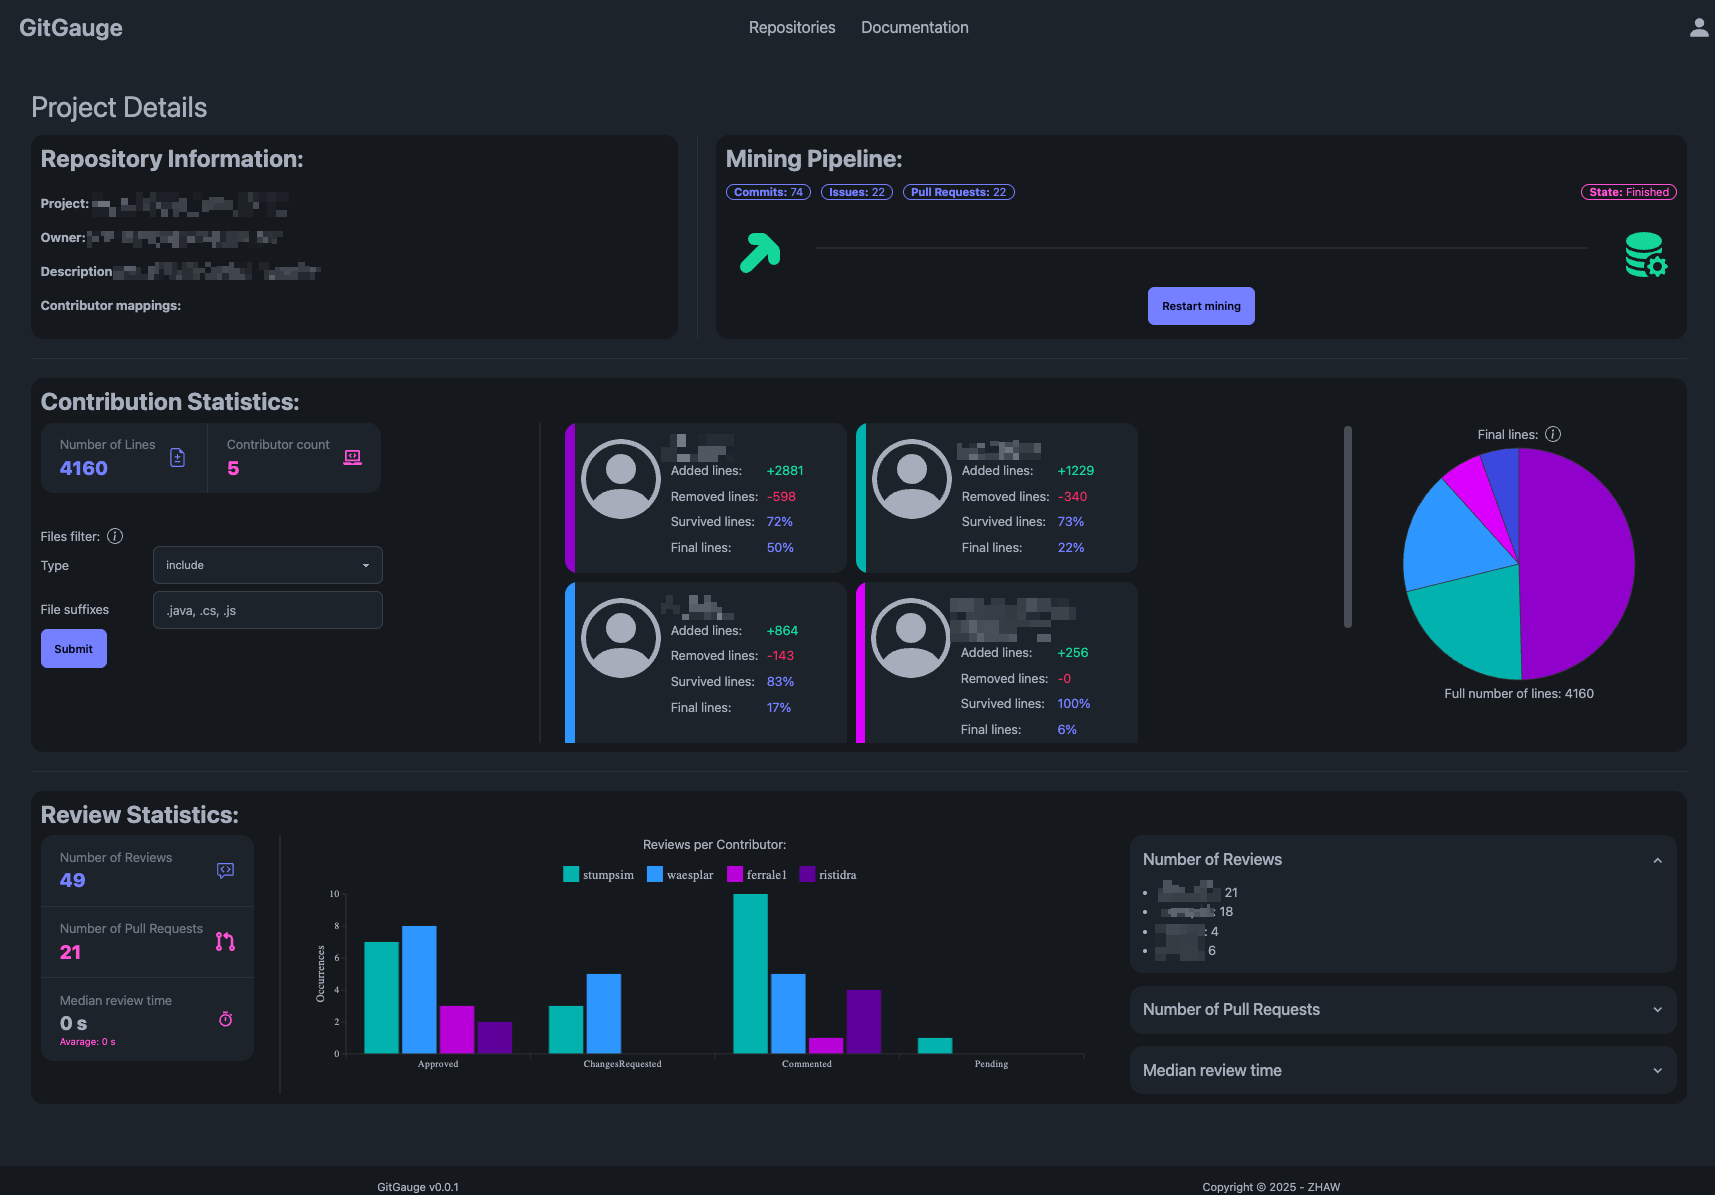
\includegraphics[width=0.8\textwidth]{Figures/giggauge-overview.png}
    \caption{Übersicht eines Projektes in GitGauge}
    \label{fig:gitgauge-project-overview}
\end{figure}

\newpage


\subsection{Vergleichbare Projekte}
Es existieren bereits mehrere Git-Analyse-Tools, die die Untersuchung von Repository-Metriken, insbesondere den Code-Reviews, ermöglichen. 

\textit{Apache Kibble} ist ein Open-Source-Projekt, welches das Minen, Aggregieren und Visualisieren von Softwareprojekten ermöglicht. Viele der bereitgestellten Metriken fokussieren sich jedoch auf die Open-Source-Aspekte eines Projektes, wie etwa die Anzahl der Autoren pro Zeitperiode. Ausserdem ist das Projekt nicht besonders aktiv, es wurden lediglich 1 Commit in den letzten 2 Jahren getätigt \parencite{noauthor_apachekibble-1_2025}. Jedoch ist das Projekt gemäss der Apache-Webseite noch aktiv \parencite{noauthor_apache_nodate}. Abbildung \autoref{fig:apache-kibble} zeigt einen Ausschnitt der offiziellen Demo. 
\begin{figure}[htbp]
    \centering
    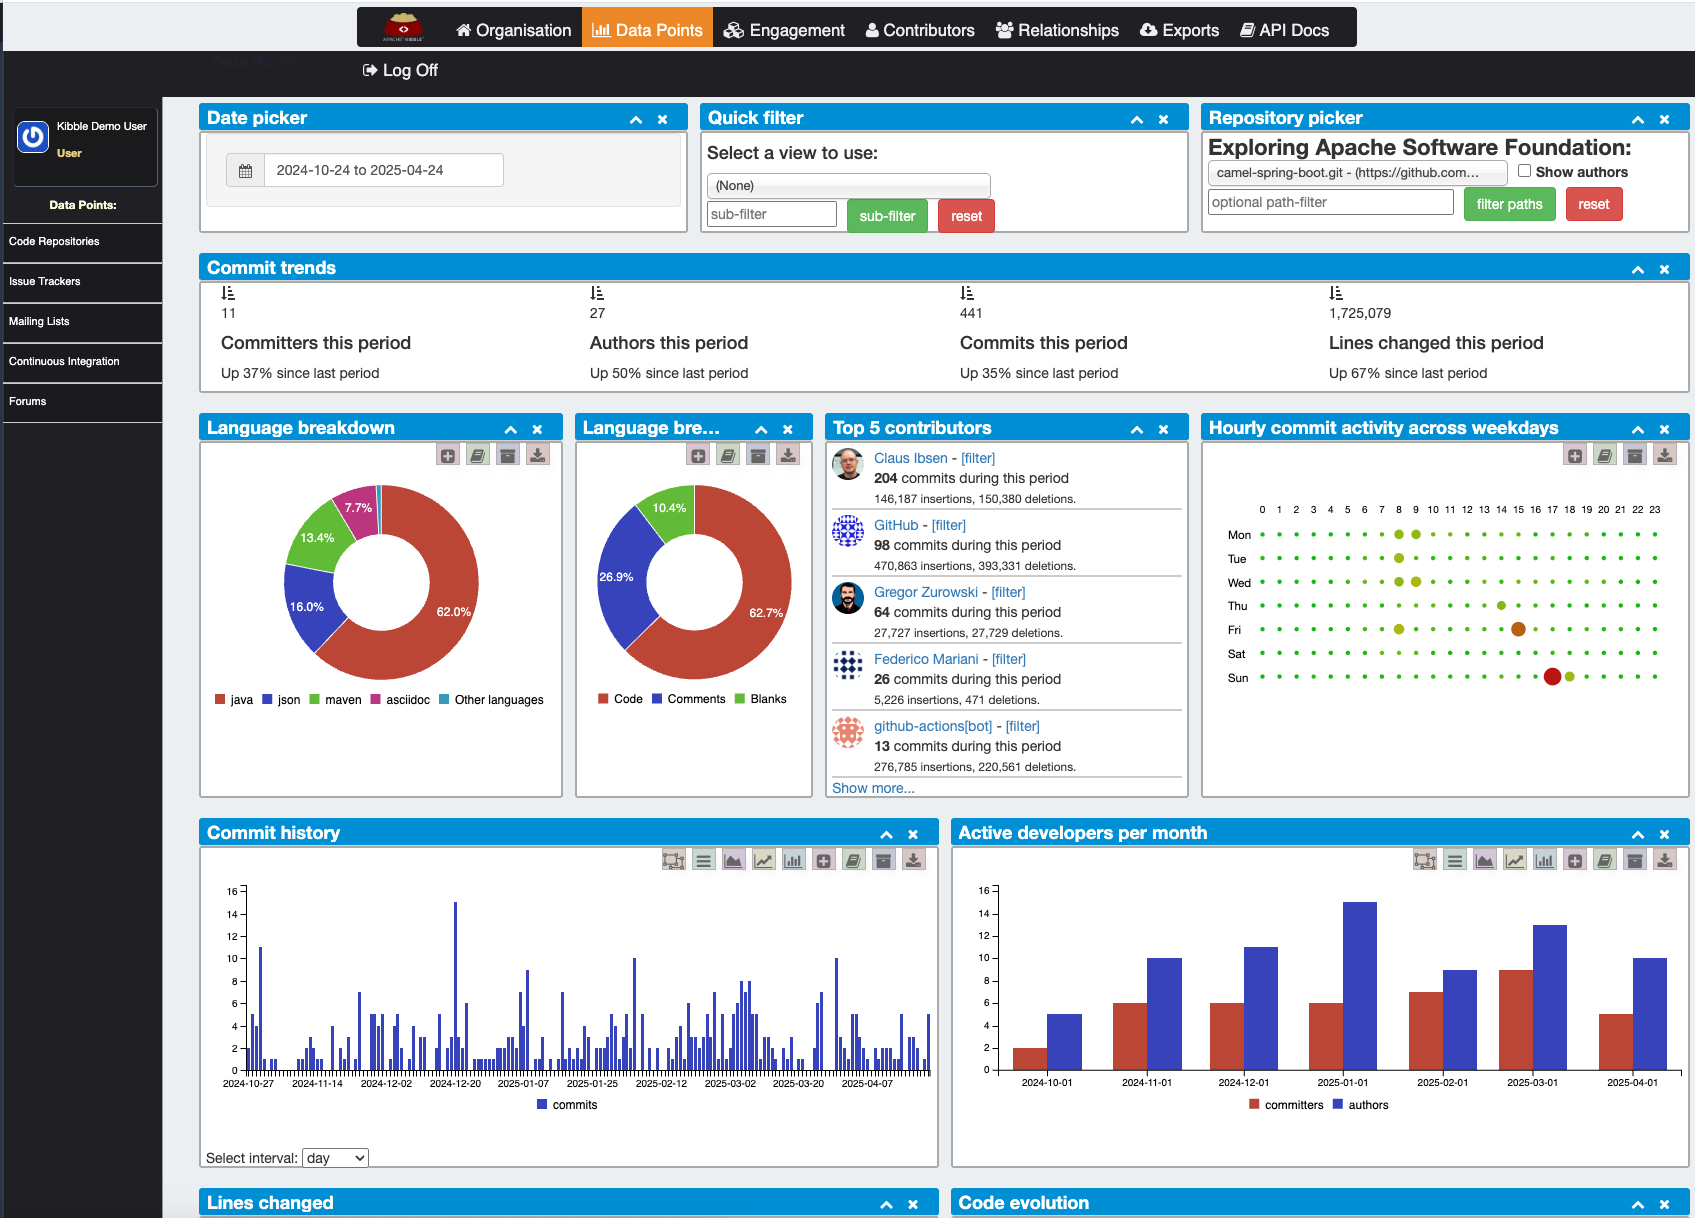
\includegraphics[width=0.8\textwidth]{Figures/apache-kibble.png}
    \caption{Screenshot der Apache Kibble-Demo \parencite{noauthor_code_nodate}}
    \label{fig:apache-kibble}
\end{figure}

\textit{Augur} ist ein Data-Engineering-Tool und REST-Webservice, welcher sich auf die Analyse von GitHub- und GitLab-Daten fokussiert. Der Hauptfokus von Augur liegt auf der Messung der allgemeinen Gesundheit und Nachhaltigkeit von Open-Source-Projekten. Das Tool sammelt und normalisiert Daten aus verschiedenen Repositories, um nützliche Metriken über den Zustand eines Projekts (GitHub-Organi\-sation) zu liefern. Diese Metriken ermöglichen eine umfassende Analyse der Entwickleraktivitäten, der Community-Dynamiken und der Stabilität von Projekten. Die Daten werden in einer relationalen Datenbank abgespeichert \parencite{noauthor_chaossaugur_nodate}. Augur ist ein Projekt der \textit{CHAOSS} (Community Health Analytics in Open-Source-Software) Community, welche selbst der Linux Foundation angehört. Die CHAOSS-Community beschäftigt sich mit der Analyse und Messung der Gesundheit und Nachhaltigkeit von Open-Source-Projekten. So werden Metriken entwickelt, die die langfristige Stabilität und das Wachstum der Projekte unterstützen sollen. Die Community verwaltet über 60 Repositories auf GitHub. \parencite{noauthor_chaoss_nodate} \parencite{noauthor_about_nodate-1}
\newpage
\textit{8Knot} ist eine Dash-Webanwendung, welche von \textit{Red Hat Open Source Program Office} entwickelt wird. Es nutzt die von Augur gesammelten Daten, um die Interaktionen der Git-Projekte zu visualisieren \parencite{noauthor_chaossaugur_nodate} \parencite{noauthor_oss-aspen8knot_2025}. 
\begin{figure}[htbp]
    \centering
    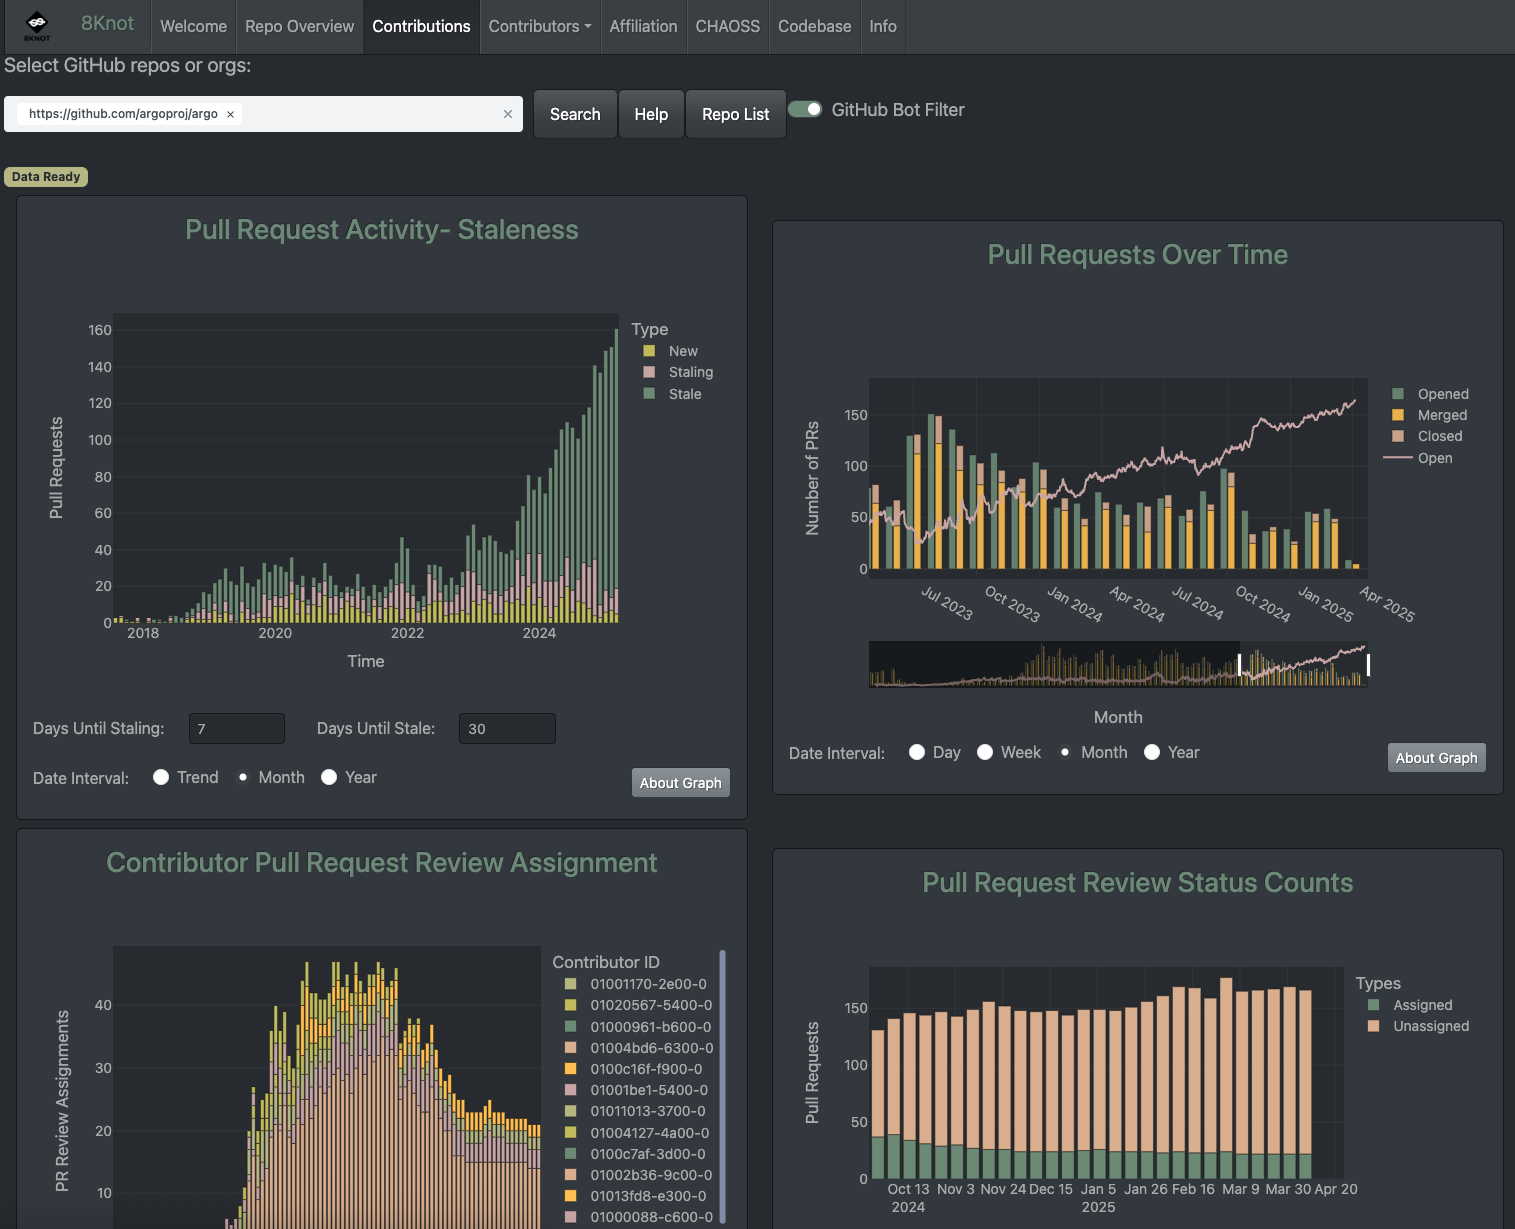
\includegraphics[width=0.9\textwidth]{Figures/augur-8knot.png}
    \caption{Analyse des Projektes Argo mittels Augur \& 8Knot \parencite{noauthor_metrixchaossio_nodate} \parencite{noauthor_argoprojargo-workflows_2025}}
    \label{fig:augur-8knot}
\end{figure}


\section{Aufgabenstellung}
Produktivitätsmetriken sollen aus Git-Repositories gewonnen werden. Aus den Daten der Repositories sollen aussagekräftige Kennzahlen für die Softwareentwicklung abgeleitet werden. Dies soll durch eine Literaturrecherche bestehender Metriken und die Entwicklung von Analysealgorithmen erfolgen.
Die offizielle Aufgabenstellung, gestellt von Michael Wahler, befindet sich im Anhang \secref{sec:OffAufgabenstellung}.
\newpage
\section{Forschungsfragen und Zielsetzung}
\label{sec:Zielsetzung}

Ziel dieser Arbeit ist es, Pull-Requests aus Projekten zu untersuchen und deren Eigenschaften hinsichtlich verschiedener Einflussfaktoren zu analysieren. Dabei stehen folgende Forschungsfragen im Vordergrund:

\forschungsfrage{forschungsfrage1}{
Besteht ein Zusammenhang zwischen der Latency eines Pull-Requests (Zeit bis zum Merge oder Schliessung) und dem Churn (Anzahl geänderter Codezeilen) des jeweiligen Pull-Requests?
}

\forschungsfrage{forschungsfrage2}{
Können die Schliessungsgründe der PRs in den Projekten ermittelt und klassifiziert werden?
}

\forschungsfrage{forschungsfrage3}{
Besteht ein Zusammenhang zwischen dem Zeitpunkt im Projektverlauf und der Review-Dauer von Pull-Requests?}


\forschungsfrage{forschungsfrage4}{
Lassen sich Patterns der Zusammenarbeit im Team erkennen, hinsichtlich der Tage, an denen die Studierenden an den Projekten arbeiten?
}

\forschungsfrage{forschungsfrage5}{
Welche Unterschiede zeigen sich in der Nutzung von Pull-Requests zwischen Teilzeit- und Vollzeitstudierenden hinsichtlich Anzahl, Umfang und Dauer?
}

\forschungsfrage{forschungsfrage6}{
Welche Unterschiede zeigen sich in den Repository-Metriken zwischen den Studentenprojekten und professionellen GitHub-Organisationen?
}

\section{Übersicht der Arbeit}
Im \autoref{Chapter2} \textit{\nameref{Chapter2}} wird das theoretische Wissen vermittelt, welches für das Verständnis dieser Arbeit notwendig ist. Dabei wird auf  Git / GitHub-spezifische Methodiken eingegangen, die untersuchten Projekte erläutert und das als Grundlage dienende Tool GitGauge erklärt.

Das \autoref{Chapter3} \textit{\nameref{Chapter3}} beschreibt die Methodik der Arbeit. Es erläutert die Vorgehensweise und beschreibt die notwendigen Metriken zur Klärung der Forschungsfragen. Des Weiteren wird die Datengrundlage aufgezeigt.


Die Ergebnisse werden im \autoref{Chapter4} \textit{\nameref{Chapter4}} dargelegt. Dabei wird auf die spezifischen Forschungsfragen eingegangen und die Analysen zur Beantwortung der Fragen dargestellt. Zusätzlich wird die Erweiterung an der GitGauge-Applikation demonstriert.

Zum Schluss folgt das \autoref{Chapter5} \textit{\nameref{Chapter5}}, in dem noch einmal auf die Forschungsfragen und deren Ergebnisse eingegangen und diese bewertet werden. Ausserdem werden mögliche Erweiterungen aufgezeigt.






% Indicate the main file. Must go at the beginning of the file.
% !TEX root = ../main.tex

%----------------------------------------------------------------------------------------
% EINLEITUNG
%----------------------------------------------------------------------------------------

\label{Chapter2} % Change X to a consecutive number; for referencing this chapter elsewhere, use \ref{ChapterX}

%----------------------------------------------------------------------------------------
% SECTION 1
%----------------------------------------------------------------------------------------

\chapter{Theoretische Grundlagen} % Main chapter title

In diesem Kapitel werden die theoretischen Grundlagen vorgestellt, die für das Verständnis dieser Arbeit notwendig sind. Zunächst werden Git und GitHub vorgestellt. Danach folgen die spezifischen Techniken, welche diese Systeme verwenden. Anschliessend werden die Projektmodule und deren Unterschiede zu Open-Source-Projekten erläutert. Zusätzlich wird das Tool GitGauge vorgestellt und dessen Architektur beschrieben.

\label{Chapter2} % Change X to a consecutive number; for referencing this chapter elsewhere, use \ref{ChapterX}

%----------------------------------------------------------------------------------------
% SECTION 1
%----------------------------------------------------------------------------------------

\section{Git \& GitHub}
Die Nutzung eines Versionskontrollsystems (VCS - version control system) ist ein zentrales Element der Softwareentwicklung. Mit einem VCS können Änderungen am Sourcecode nachverfolgt und bei Bedarf eine frühere Version des Projekts wiederhergestellt werden. Die Nutzung eines VCS ermöglicht ausserdem, dass mehrere Entwickler parallel am gleichen Code arbeiten können, indem die Änderungen inklusive deren Urheber sowie Zeitpunkt festgehalten werden. \parencite{noauthor_informationen_2025} 

Mit der Nutzung einer verteilten Versionsverwaltung (DVCS - distributed version control system) wird kein zentrales Repository mehr verwendet. Jeder Entwickler verfügt über eine Kopie des Projektes inklusive des gesamten Projektverlaufs. Änderungen können lokal implementiert werden. Eine Verbindung zum Server wird nur für das Synchronisieren von Änderungen notwendig. \parencite{noauthor_informationen_2025} 

Git ist heute das am meisten verbreitete DVCS-System. Es wurde von Linus Torvalds für die Entwicklung des Linux-Kernels entwickelt \parencite{zack_git_2018}. Git bezeichnet ein Projekt als ein Git-Repository, wobei der Verlauf als eine Reihe von Snapshots (Commits) modelliert wird. Diese Commits sind in unterschiedlichen Branches organisiert, welche die parallele Entwicklung ermöglichen. Die Verwendung von Branches ermöglicht die parallele Entwicklung von Bugs, neuen Features etc., ohne dass es zu gegenseitigen Beeinträchtigungen kommt. Diese unterschiedlichen Branches werden anschliessend gemerged\footnote{Abgeleitet vom englischen Verb merge}. \parencite{noauthor_informationen_2025}   

Mit dem Erfolg von Git entstanden Dienste und Anbieter, welche Git-Repositories online zur Verfügung stellen und zusätzliche Kollaborationstools anbieten. GitHub ist der bekannteste und auch am meisten verwendete Hosting-Dienst \parencite{noauthor_team_nodate}. Auf GitHub können Entwickler ihr Git-Repository hosten, Änderungen vorschlagen und diskutieren, Fehler (Issues) tracken. GitHub bietet eine Weboberfläche, welche für das Einsehen des Codes, aber auch für das Erstellen von Pull-Requests und Issues verwendet werden kann. Zusätzlich kann der CI/CD-Prozess (Continuous Integration/Continuous Deployment – automatisiertes Testen, Bauen und Ausrollen von Software) direkt mittels GitHub-Actions abgebildet werden. \parencite{noauthor_informationen_2025}  

\section{Pull-Request} 
Ein Pull-Request ist ein Vorschlag, Änderungen von einem Branch oder Fork in einen anderen Branch zusammenzuführen. In einem typischen Entwicklungsworkflow erstellt der Entwickler für eine Änderung einen neuen Branch, committet dort seine Arbeit und erstellt anschliessend einen Pull-Request. Ein Pull-Request enthält dabei die durchgeführten Codeänderungen sowie eine Beschreibung zur Änderung. Die Unterschiede (Diffs) zwischen Quell- und Zielbranch werden dabei übersichtlich aufgezeigt. \parencite{noauthor_about_nodate}

Pull-Requests spielen für den Code-Review und die Diskussion innerhalb des Entwicklungsprozesses eine wichtige Rolle. So bietet ein Pull-Request eine Basis zur Diskussion, indem Teammitglieder den Code begutachten, kommentieren und auch Änderungen vorschlagen können \parencite{atlassian_pull_nodate}. Viele Entwicklerteams richten daher verbindliche Review-Prozesse ein, bei denen ein Pull-Request erst dann gemerged werden kann, wenn dieser von mindestens einer Person genehmigt wurde \parencite{jiang_how_2022}.

Durch das Konfigurieren von automatischen Checks mittels CI/CD können sowohl Anforderungen an die Softwarequalität (zum Beispiel durch das automatisierte Ausführen von Tests oder statischen Codeanalysen) als auch an den Entwicklungsprozess automatisiert überprüft werden \parencite{kinsman_how_2021}. Dazu gehört beispielsweise die Überprüfung, ob alle Commits mit einem Signed-off-by versehen sind, was in vielen Projekten zur Einhaltung des Developer Certificate of Origin (DCO) verpflichtend ist. Diese Massnahmen stellen sicher, dass sowohl die technische Qualität des Codes als auch rechtliche Rahmenbedingungen eingehalten werden, bevor ein Pull-Request gemerged wird. \parencite{holtgrave_attributing_2025} 

Am Ende eines Pull-Requests wird dieser entweder akzeptiert und in den zuvor ausgewählten Branch integriert (Merged) oder geschlossen (Close)\parencite{noauthor_merging_nodate}\parencite{noauthor_closing_nodate}. Die Akzeptanz kann dabei auf zwei Arten erfolgen. Entweder wird der Merge-Button durch den Antragsteller oder ein anderes Teammitglied direkt angeklickt oder es erfolgt eine Genehmigung (Approval) \parencite{noauthor_merging_nodate}\parencite{noauthor_reviewing_nodate}. Die Genehmigung ist eine Aktion, welche auf einem Pull-Request ausgeführt werden kann. Es besteht auch die Möglichkeit, diese Aktion zu erzwingen, und somit dürfen die Änderungen erst zusammengeführt werden, wenn ein anderes Teammitglied den Pull-Request genehmigt hat \parencite{noauthor_approving_nodate}.

\subsection{Git-Squashing}
\label{sec:GitSquashing}
Mit Git-Squashing wird die Praxis bezeichnet, mehrere Commits zu einem Commit zusammenzuführen, bevor diese in den Zielbranch gemerged werden. Dies kann entweder manuell durch ein interaktives Rebase über die Git-Kommandozeile oder automatisch erfolgen, indem beim Mergen des Pull-Requests die Option Squash-Commits ausgewählt wird. Je nach Plattform kann die Option zum automatischen squashing von Commits beim Mergen des Pull-Requests unterschiedlich bezeichnet sein \parencite{noauthor_about_nodate}\parencite{noauthor_squash_nodate}. \parencite{noauthor_git_nodate} 

Daraus ergibt sich, dass alle Änderungen eines Feature-Branches im Zielbranch zusammengeführt werden, ohne die gesamte Historie zu übernehmen. Oftmals dient dies dazu, die Lesbarkeit des Projektverlaufs zu verbessern oder fehlerhafte Commits auszublenden. Darüber hinaus kann das Reverten von Commits erleichtert werden, da eine flache Git-Historie, die nur eine zusammengefasste Reihe von Commits enthält, beim Zurücksetzen von Änderungen Vorteile bietet \parencite{just_switching_2016}. \parencite{codoban_comparative_2015}

Nachteil ist der Verlust von Informationen über die schrittweise Entwicklung eines Features. Die Commits der jeweiligen Feature-Entwicklung und deren Nachrichten gehen verloren, was die Transparenz des Entwicklungsprozesses einschränkt. \parencite{codoban_comparative_2015}

\section{Branching-Strategien}
Es existieren verschiedene Branching-Strategien. Die für diese Studie erwähnenswerten Strategien sind der Git Flow und der GitHub Flow. \parencite{priyanka_gowdaashwath_narayana_gowda_git-branching-and-release-strategies_2022} 
\subsection{Git Flow}
\label{sec:GitFlow}
Der Git Flow wurde 2010 von Vincent Driessen vorgestellt, als ein robustes Branch\-ing-Konzept, welches für jedes Projekt passen soll \parencite{priyanka_gowdaashwath_narayana_gowda_git-branching-and-release-strategies_2022}.
Diese Strategie besteht aus zwei Hauptbranches:
\begin{itemize}
    \item Master: Beinhaltet den produktionsreifen Code  
    \item Develop: Integrationsebene für neue Funktionen
\end{itemize}
und drei Hilfsbranches:
\begin{itemize}
    \item Feature: Entwicklung von neuen Funktionen
    \item Hotfix: Für kritische Fehler in der Produktion
    \item Release: Vorbereitungsebene für Funktionen die produktiv werden sollen.
\end{itemize}
Neue Funktionen werden in Feature-Branches entwickelt und nach Beendigung in den Develop-Branch gemerged. Der Develop-Branch wird dann in den jeweiligen Release-Branch und schlussendlich in den Main-Branch gemerged. Falls es in der Produktion zu einem kritischen Fehler kommt, welcher nicht bis zum neuen Release warten kann, wird jener in einem Hotfix-Branch behoben und zurück in den Main-Branch gemerged.
\parencite{priyanka_gowdaashwath_narayana_gowda_git-branching-and-release-strategies_2022}

\subsection{GitHub Flow}
\label{sec:GitHubFlow}
Die GitHub Flow-Strategie ist eine vereinfachte und leichtgewichtige Methode. Sie besteht aus den folgenden Branches:
\begin{itemize}
    \item Main: Beinhaltet den produktionsreifen Code  
    \item Feature: Entwicklung von neuen Funktionen
\end{itemize}
Auch in dieser Strategie werden neue Funktionen in einem Feature Branch entwickelt. Diese werden jedoch nach Abschluss, via Pull-Requests, direkt in den Main-Branch gemerged.
\parencite{priyanka_gowdaashwath_narayana_gowda_git-branching-and-release-strategies_2022}

% Weiss nicht ob wir diese reinnehmen wollen oder nicht
% \subsection{GitLab Flow}
% Der GitLab Flow befindet sich zwischen der Git- und der GitHub-Flow-Methode. 
% \begin{itemize}
%     \item Production: Beinhaltet den produktiven Code  
%     \item Staging: Umgebungsspezifischeebene
%     \item Development: Integrationsebene für neue Funktionen
%     \item Feature: Entwicklung von neuen Funktionen
% \end{itemize}
% Neue Funktionen werden ebenfalls in den Feature Branches entwickelt. Diese werden dann in den Development Branch gemerged. Danach werden sie in die entsprechenden Staging Branches gemerged und sobald sie produktionsreif sind, in den Production Branch gemerged.
% \parencite{priyanka_gowdaashwath_narayana_gowda_git-branching-and-release-strategies_2022}

% \subsection{Trunked-based development}
% Diese Strategie basiert auf kurzlebigen Branches, welche dann in den Main-Branch integriert werden.
% \begin{itemize}
%     \item Main: Beinhaltet den Produktionsreifen Code 
%     \item Kurzlebiger Branch: Kleine Änderungen, keine ganzen Features
% \end{itemize}
% Bei dieser Strategie werden kleine Änderungen über kurzlebige Branches in den Main Branch gebracht. Dabei werden nicht ganze Features in einem Branch implementiert, sondern diese werden in kleine Stückchen aufgeteilt.
% \parencite{atlassian_trunk-based_nodate}

\section{Vergleichbare Arbeiten}
In diesem Kapitel wird ein Überblick über bestehende Arbeiten im Bereich der Pull-Request-Forschung gegeben. Dabei werden sowohl zeitliche Aspekte (Latency) als auch Erkenntnisse zu Akzeptanzfaktoren sowie existierende Analysewerkzeuge für Git-Repositories betrachtet.

\subsection{Pull-Request-Latency}
\label{sec:PullRequestDauer}
Es existieren bereits diverse Studien, die sich mit der Analyse von Pull-Requests befassen. In der Literatur werden verschiedene Faktoren untersucht, die die Dauer von Pull-Requests beeinflussen. Zusammenfassend kommen die Studien zum Schluss, dass die Pull-Request-Laufzeit von verschiedenen Faktoren, wie der Diskussion, der Reputation des Erstellers, der Team-Auslastung, der ersten menschlichen Reaktion und von Continuous Integration, wie beispielsweise dem Abwarten von automatisierten Tests, abhängig ist. Es existieren jedoch widersprüchliche Aussagen bezüglich der Abhängigkeit der Laufzeit von der PR-Grösse. \parencite{yu_wait_2015}\parencite{hasan_understanding_2023}\parencite{kudrjavets_small_2022}\parencite{bernardo_studying_2018}

Yue Yu u.a.\parencite{yu_wait_2015} analysieren mit linearen Regressionsmodellen relevante Faktoren bei GitHub-Projekten. Die Ergebnisse zeigen, dass sowohl die Grösse eines Pull-Requests, gemessen an der Anzahl der Änderungen, als auch die Länge der Diskussion die Laufzeit beeinflussen. Des Weiteren wird ein Zusammenhang zwischen der Reputation des Erstellers und der Dauer nachgewiesen. Darüber hinaus wird ein Zusammenhang zwischen der Grösse des Teams, der Auslastung, definiert als Anzahl offener Pull-Requests, sowie der Zeit bis zur ersten menschlichen Reaktion auf den Pull-Request festgestellt. Zusätzlich zeigt die Studie, dass CI-Faktoren einen signifikanten Einfluss haben, wie beispielsweise das Warten auf automatisierte Tests.~\parencite{yu_wait_2015}

Das Paper von Kazi Amit Hasan u.a.\parencite{hasan_understanding_2023} befasst sich spezifischer mit der ersten Reaktion auf einen Pull-Request anhand von Open-Source-Projekten. In diesem Zusammenhang sind Reaktionen definiert in Form eines Kommentars auf einen Pull-Request oder eines Code-Review-Kommentars auf einen Pull-Request. Es wird festgestellt, dass die erste Antwort eines Bots kaum Auswirkungen auf die Dauer hat, die erste Antwort eines Menschen jedoch einen grossen Einfluss hat. Die Dauer der ersten menschlichen Reaktion ist in der Hälfte der Fälle auf neun Faktoren zurückzuführen. Diese neun Faktoren sind die Länge der Beschreibung, die Anzahl Commits, die Anzahl bearbeiteter Files, die Anzahl geänderter Codezeilen, die Anzahl hinzugefügter Codezeilen,  ob eine Person auf dem Pull-Request markiert wurde, die Anzahl offener Pull-Requests, die Anzahl der bisherigen Pull-Requests des Entwicklers und der Anteil der Teammitglieder, mit denen der Entwickler in den letzten drei Monaten interagiert hat. Insbesondere bei Pull-Requests mit längeren Beschreibungen und komplexeren Code-Änderungen dauert die erste menschliche Reaktion länger. Ebenfalls wird ein Zusammenhang bezüglich der Auslastung, also den offenen PRs und der ersten Interaktion festgestellt. Ein weiteres Resultat ihrer Recherche zeigt auf, dass Verfasser mit weniger Erfahrung (Anzahl erfasster PRs) und fehlende Interaktionen mit Projektmitgliedern ebenfalls zu längeren ersten menschlichen Reaktionen führen können.\parencite{hasan_understanding_2023} 

Beide oben beschriebenen Studien stellen einen Zusammenhang zwischen der Grösse eines Pull-Requests und dessen Dauer fest \parencite{yu_wait_2015}\parencite{hasan_understanding_2023}. Die Studie von Gunnar Kudrjavets, Nachiappan Nagappan und Ayushi Rastogi  \parencite{hasan_understanding_2023}, die sich spezifisch mit dieser Thematik befasst, gelangt zu dem Schluss, dass kein Zusammenhang zwischen diesen beiden Aspekten festgestellt werden kann. Alle drei Studien basieren auf populären GitHub-Projekten, jedoch unterscheiden sich die Auswahlkriterien der Projekte. Yu u.a.\parencite{yu_wait_2015} beschränkten ihre Untersuchung auf GitHub-Projekte, die mindestens 1'000 Pull-Requests enthalten und den CI-Dienst Travis-CI verwenden. Travis-CI war zum Zeitpunkt der Studie der am weitesten verbreitete CI-Dienst auf GitHub. Insgesamt wurden 40 Repositories ausgewählt, verteilt auf fünf der populärsten Programmiersprachen (Ruby, Python, JavaScript, Java und C++). Hasan u.a.\parencite{hasan_understanding_2023} analysierten zehn populäre Open-Source-Projekte mit einer grosser Pull-Request-Historie, basierend auf einem von Zhang u.a.\parencite{zhang_pull_2022} erstellten Benchmark-Datensatz. Dieser enthält über drei Millionen geschlossene Pull-Requests aus mehr als 11'000 Projekten. Für ihre Analyse berücksichtigten Hasan u.a. nur Pull-Requests mit mindestens einem Kommentar. Kudrjavets u.a.\parencite{kudrjavets_small_2022} wählten 100 der populärsten und aktiv entwickelten Repositories auf GitHub aus, wobei jeweils zehn Projekte aus den zehn beliebtesten Programmiersprachen (basierend auf GitHub-Statistiken von Oktober 2019 bis September 2020) berücksichtigt wurden. Die Auswahl wurde anhand der Anzahl an Stars, Forks und Pull-Requests getroffen.

João Helis Bernardo, Daniel Alencar Da Costa und Uirá Kulesza \parencite{bernardo_studying_2018} zeigen, dass Projekte, die Continuous-Integration eingeführt haben, danach Pull-Requests mit längeren Laufzeiten hatten.

\subsection{Pull-Request-Akzeptanz}
Über die Einflussfaktoren der Akzeptanz von Pull-Reque\-sts existieren bereits mehrere Studien.
So zeigen diverse Untersuchungen, dass die Akzeptanz eines Pull-Requests von mehreren technischen als auch sozialen Faktoren abhängig ist \parencite{gousios_exploratory_2014}. \
Eine Studie, die über 40'000 Pull-Requests in Projekten mit unterschiedlichen Programmiersprachen (Java, Python, C etc.) analysierte, stellt fest, dass die Code-Qualität nur einen geringen Einfluss auf die Akzeptanzrate hat \parencite{kuhejda_pull_2023}.

Die Grösse eines Pull-Requests (Umfang der Code-Änderungen) ist ein technisches Merkmal, das in der Literatur häufig erwähnt wird. Hierzu gibt es in der Forschung unterschiedliche Ergebnisse. So stellt eine Studie, die manuell über 300 Pull-Requests der Eclipse- und Mozilla-Foundation untersuchte, fest, dass nur 0.3\,\% aller abgelehnten Pull-Requests aufgrund ihrer zu grossen Grösse abgelehnt wurden \parencite{tao_writing_2014}. Andere Untersuchungen ergaben, dass umfangreiche Pull-Requests tendenziell seltener akzeptiert werden. Ein statistisches Modell zeigt, dass mit jeder zusätzlichen Grössenordnung die Wahrscheinlichkeit einer Akzeptanz um 26\,\% sinkt. Allerdings wird betont, dass die Grösse eines Pull-Re\-quests allein selten der Ablehnungsgrund ist. Vielmehr erschweren grosse PRs die Bewertung und führen dann zu einer Ablehnung, wenn zusätzliche Kosten, Unklarheiten oder Qualitätsmängel auftreten könnten. Eine Studie, die sich auf Mozilla-Projekte konzentrierte, stellt fest, dass Entwickler häufig glauben, dass die Grösse eines Pull-Requests entscheidend für die Akzeptanz ist. \parencite{tsay_influence_2014}

Darüber hinaus haben auch zeitliche und prozessuale Faktoren einen grossen Einfluss auf die PR-Akzeptanz. Eine Untersuchung der zeitlichen Dimension von PR-Entscheidungen zeigt, dass sich die Bedeutung einzelner Variablen im Verlauf eines PR-Lebenszyklus ändern kann. Die wichtigsten Variablen für die finale Merge-Entscheidung (bei bereits abgeschlossenen PRs) sind zwar auch für offene Pull-\linebreak Requests relevant, können jedoch gegenteilig wirken. Das bedeutet, dass bestimmte Merkmale wie etwa die Grösse, Tests oder die Diskussion über den PR in früheren Phasen anders bewertet werden als im Endergebnis. \parencite{west_temporal_2023}

Soziale Faktoren spielen ebenfalls eine wichtige Rolle. Pull-Requests von Entwicklern, die eine soziale Bindung zum Projekt haben (durch vorherige Mitarbeit oder durch den persönlichen Kontakt mit einem Projekt-Maintainer), werden deutlich häufiger akzeptiert. Ebenso begünstigt das vorherige Mitwirken im Projekt, etwa durch frühere PRs oder Issues, die Annahme eines Pull-Requests. Umfangreiche Diskussionen reduzieren jedoch wiederum die Wahrscheinlichkeit einer Akzeptanz~ \parencite{tsay_influence_2014}.

Insgesamt zeigen die Studien, dass technische Merkmale (Änderungsumfang, Code-Qualität, Tests etc.) stets im Zusammenspiel mit sozialen und prozessbezogenen Faktoren betrachtet werden müssen, um die Akzeptanz von Pull-Requests zu erklären.

\subsection{Vergleichbare Tools}
Es existieren bereits mehrere Git-Analyse-Tools, die die Untersuchung von Reposi\-tory-Metriken, insbesondere den Code-Reviews, ermöglichen. 

Apache Kibble ist ein Open-Source-Projekt zur Analyse von Softwareprojekten \linebreak durch Mining, Aggregation und Visualisierung relevanter Metriken. Der Fokus liegt dabei jedoch stark auf allgemeinen Open-Source-Aspekten, wie beispielsweise der Anzahl aktiver Entwickler oder der Aktivität über Zeitperioden. Für spezifische Fragestellungen wie etwa die detaillierte Analyse von Pull-Request-Latencies, Review-Dauern oder studentischen Arbeitsmustern bietet Kibble nur begrenzte Unterstützung. Ein weiterer Schwachpunkt ist die geringe Projektaktivität. In den letzten zwei Jahren wurde für den Server nur ein einziger Commit durchgeführt \parencite{noauthor_apachekibble-1_2025}. Die Scanner werden von Zeit zu Zeit aktualisiert, jedoch ist auch hier die Projektaktivität nur minimal \parencite{noauthor_apachekibble-scanners_2024}. Dies wirft Zweifel an der langfristigen Wartung und Weiterentwicklung des Tools auf, auch wenn es laut Apache-Webseite offiziell noch als aktiv gilt \parencite{noauthor_apache_nodate}. \autoref{fig:apache-kibble} zeigt einen Ausschnitt der offiziellen Demo. \parencite{sally_apache_2018}\parencite{noauthor_setting_nodate}
\begin{figure}[htbp]
    \centering
    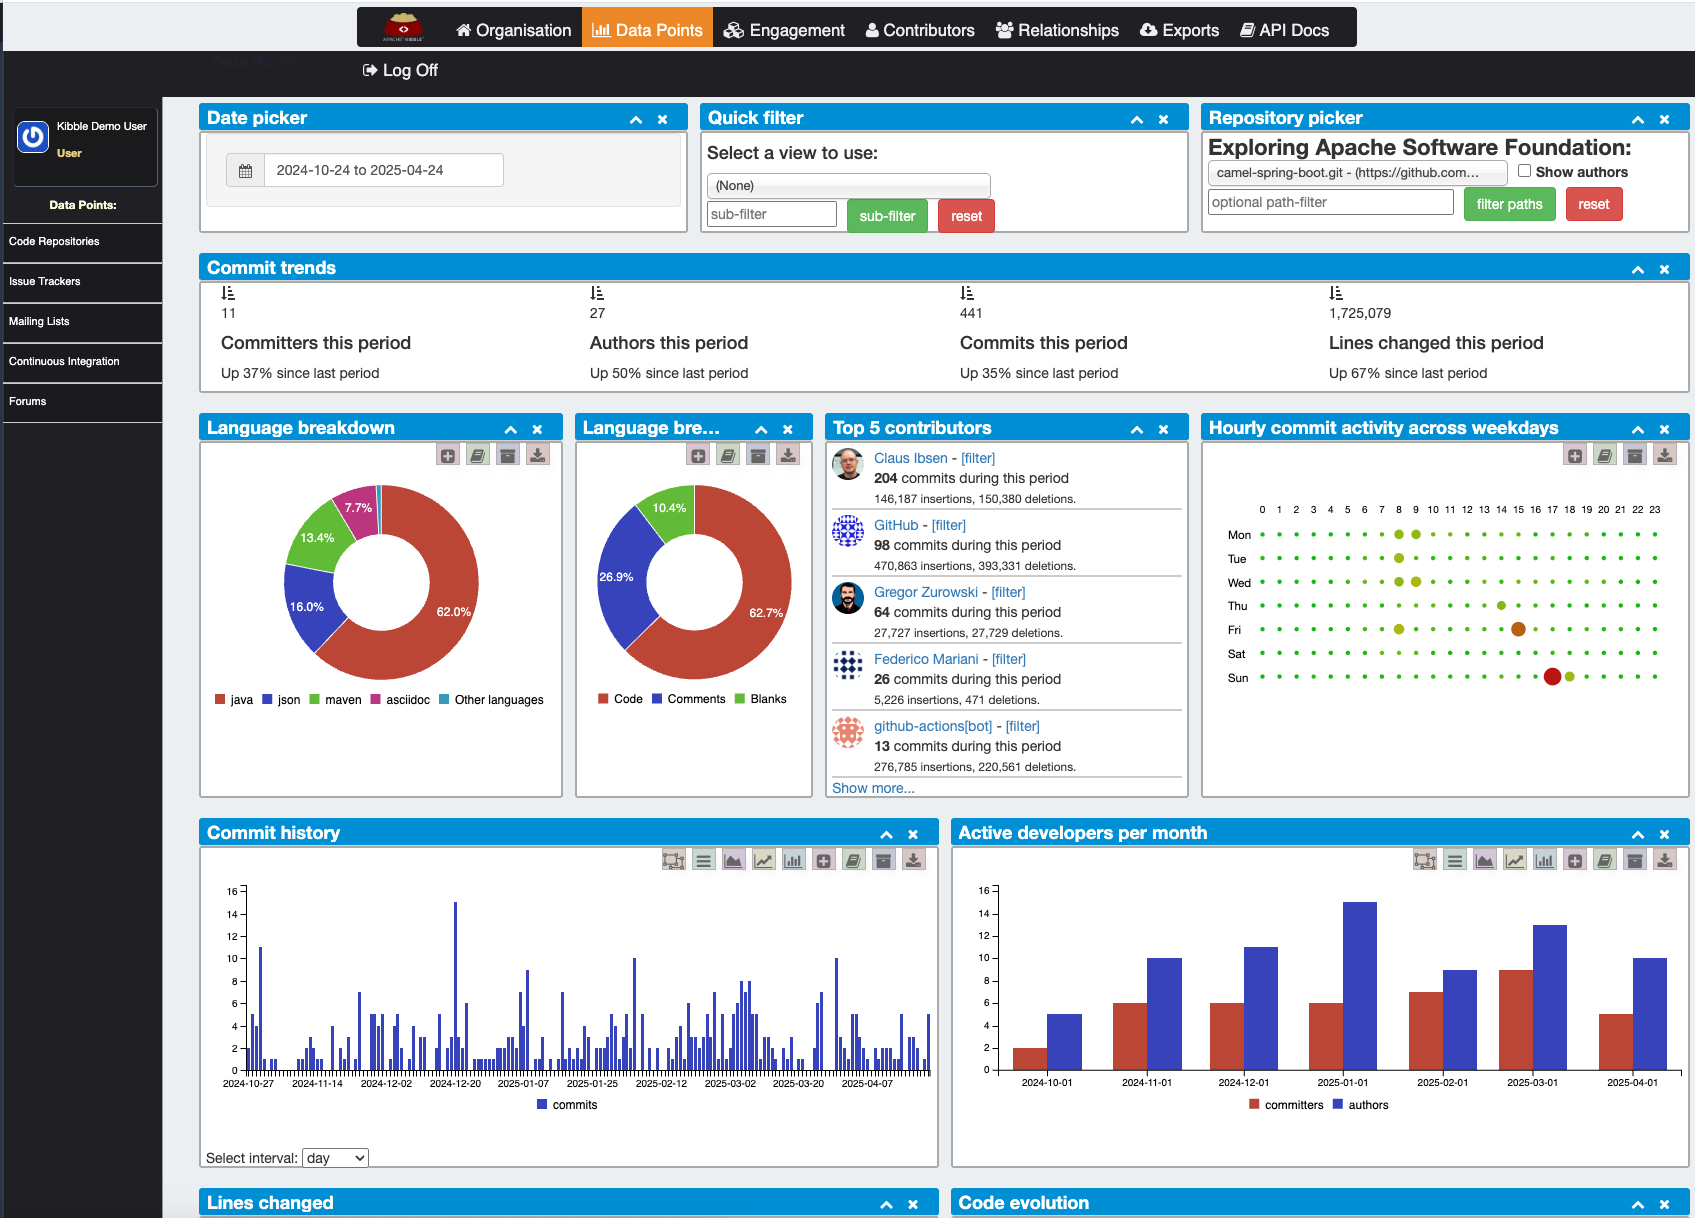
\includegraphics[width=0.9\textwidth]{Figures/apache-kibble.png}
    \caption{Screenshot der Apache Kibble-Demo \parencite{noauthor_code_nodate}}
    \label{fig:apache-kibble}
\end{figure}

\newpage
Augur ist ein Data-Engineering-Tool und REST-Webservice, welcher sich auf die Analyse von GitHub- und GitLab-Daten fokussiert. Der Hauptfokus von Augur liegt auf der Messung der allgemeinen Gesundheit und Nachhaltigkeit von Open-Source-Projekten. Das Tool sammelt und normalisiert Daten aus verschiedenen Repositories, um nützliche Metriken über den Zustand eines Projekts (GitHub-Organi\-sation) zu liefern. Diese Metriken ermöglichen eine umfassende Analyse der Entwickleraktivitäten, der Community-Dynamiken und der Stabilität von Projekten. Die Daten werden in einer relationalen Datenbank abgespeichert. Augur ist ein Projekt der CHAOSS (Community Health Analytics in Open-Source-Software) Community, welche selbst der Linux Foundation angehört. Die CHAOSS-Community beschäftigt sich mit der Analyse und Messung der Gesundheit und Nachhaltigkeit von Open-Source-Projekten. So werden Metriken entwickelt, die die langfristige Stabilität und das Wachstum der Projekte unterstützen sollen. Die Community verwaltet über 60 Repositories auf GitHub \parencite{noauthor_chaoss_nodate}.
Obwohl Augur eine breite Palette an Metriken anbietet und als Teil der CHAOSS-Community kontinuierlich weiterentwickelt wird, eignet sich das Tool primär für die Analyse grossflächiger Open-Source-Organisationen. Es fehlen jedoch Funktionalitäten, die für kleinere, zeitlich begrenzte Projekte, wie etwa die Projektmodule, entscheidend sind. Dazu zählen unter anderem die Analyse der Pull-Request-Latency im zeitlichen Projektverlauf, die Erkennung von Arbeitstagen der Entwickler oder die spezifische Kategorisierung von PR-Schliessgründen. Auch die Visualisierung ist eher auf generelle Projektgesundheit als auf relevante Einblicke in Teamprozesse ausgelegt. \parencite{noauthor_about_nodate-1}\parencite{noauthor_chaossaugur_nodate}


8Knot ist eine Dash-Webanwendung, welche von Red Hat Open Source Program Office entwickelt wird \parencite{noauthor_measuring_nodate}. Es nutzt die von Augur gesammelten Daten, um die Interaktionen der Git-Projekte zu visualisieren \parencite{noauthor_chaossaugur_nodate}\parencite{noauthor_oss-aspen8knot_2025}. \autoref{fig:augur-8knot} zeigt die Analyse eines Beispielprojektes mittels Augur und 8Knot. 
\begin{figure}[htbp]
    \centering
    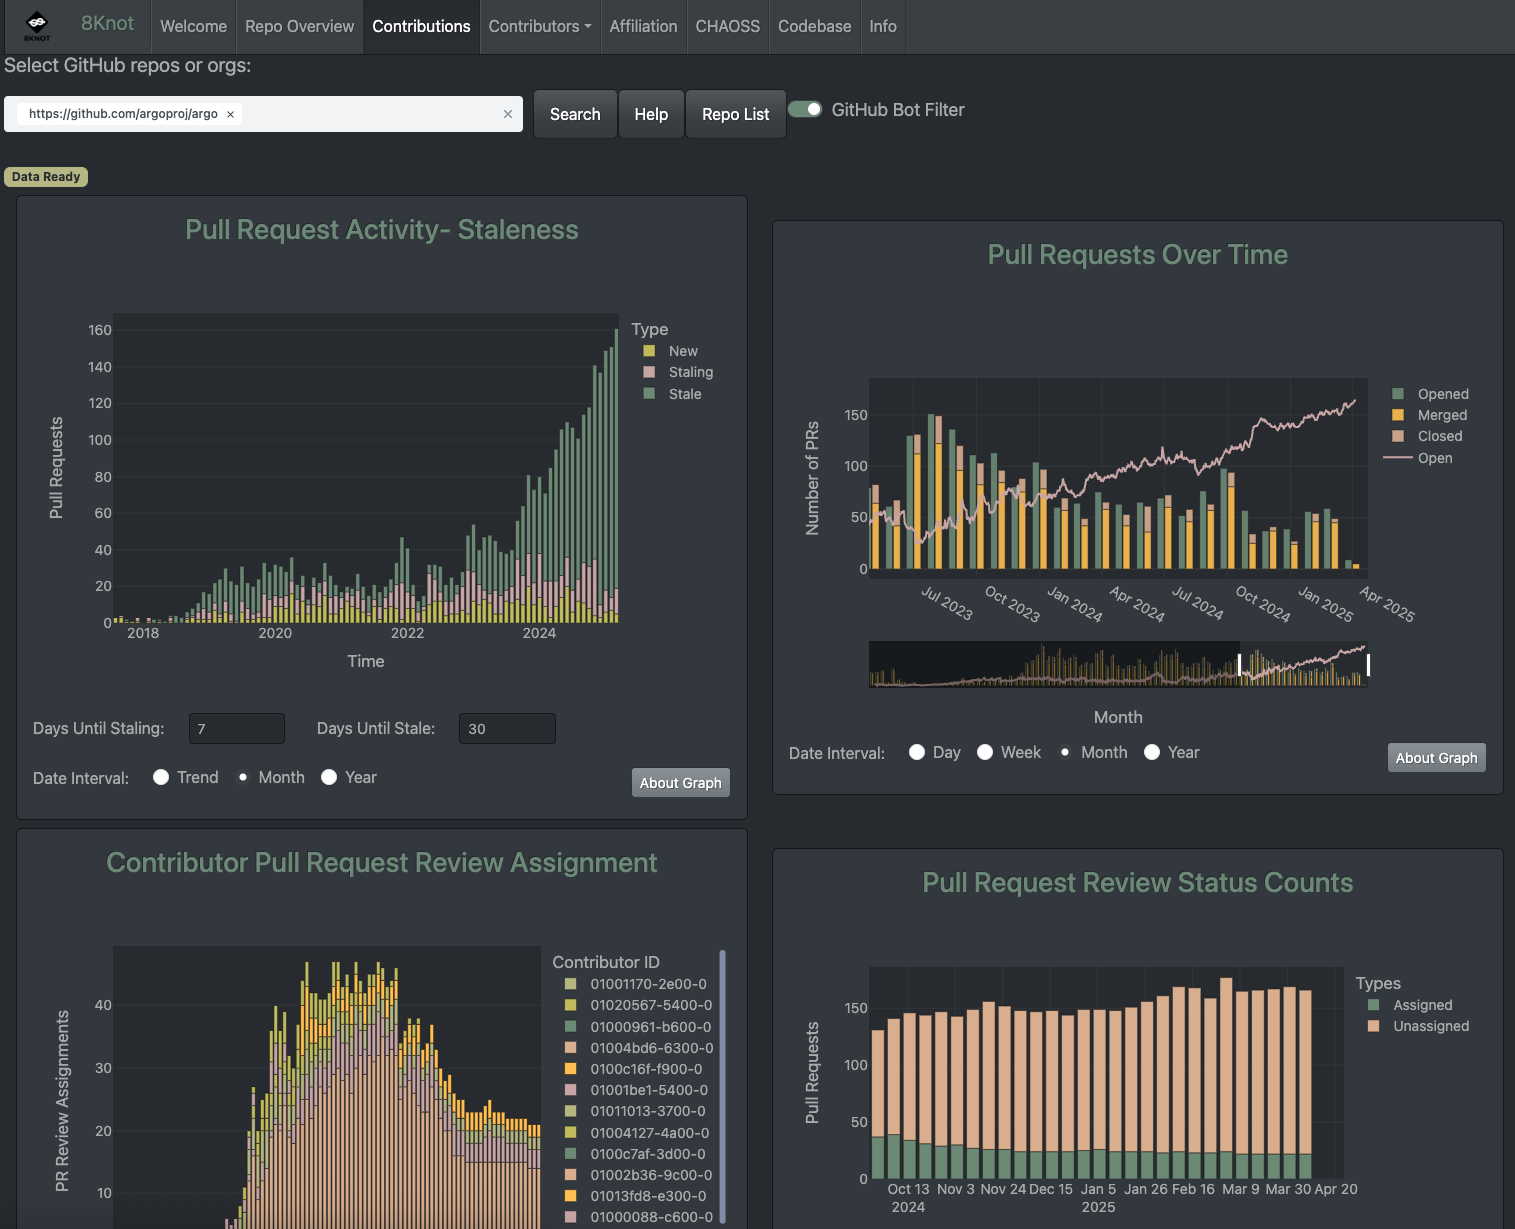
\includegraphics[width=0.9\textwidth]{Figures/augur-8knot.png}
    \caption{Analyse des Projektes Argo mittels Augur \& 8Knot \parencite{noauthor_metrixchaossio_nodate}\parencite{noauthor_argoprojargo-workflows_2025}}
    \label{fig:augur-8knot}
\end{figure}




\section{Projektmodule}
\label{sec:Projektmodule} 
Wie im Abschnitt \secref{sec:Ausgangslage} beschrieben, finden an der ZHAW Projektmodule statt. Im  Informatikstudium werden vier Projektmodule (PM) durchgeführt. In diesen Modulen geht es darum, Erfahrungen im Management und der Realisierung von Softwareprojekten im Team zu sammeln \parencite{noauthor_modul_nodate}. 

Im Rahmen des Projektmodul 1 werden in Vierergruppen drei Projekte in jeweils drei Wochen durchgeführt. In diesen Projekten wird bereits mit Git gearbeitet, das Arbeiten mit Pull-Requests wird jedoch noch nicht forciert und ist daher für diese Studie irrelevant. Ab dem PM2 werden Pull-Requests vorausgesetzt. Das Projektmodul 2 hat sich im Laufe der analysierten Repositories verändert. In der früheren Version werden zwei Projekte in Vierergruppen in jeweils vier Wochen und ein Projekt in einer Zweiergruppe innerhalb von drei Wochen durchgeführt. Dabei wird im ersten Projekt das Pen \& Paper-Spiel Racetrack als textbasiertes Spiel umgesetzt. Im zweiten Projekt erhalten die Studierenden ein fertiges Chatprogramm, welches analysiert, verbessert und repariert werden muss. Als letztes Projekt soll eine kleine JavaFX-Applikation zu einem selbst gewählten Thema umgesetzt werden. In der späteren Version wurde das zweite Projekt, das Chatprogramm, welches 3 Wochen dauert, entfernt und dafür das eigene Projekt um 2 Wochen verlängert. Im dritten Projektmodul wird innerhalb eines Semesters in zufällig ausgewählten Gruppen von circa fünf Personen ein selbst gewähltes Projekt umgesetzt. Dabei geht es darum, ein Projekt von der Vision bis zur lauffähigen Anwendung in einem iterativen und inkrementellen Prozess der Software-Entwicklung zu realisieren. Das letzte Projektmodul umfasst ebenfalls die Umsetzung eines eigenständig gewählten Projekts innerhalb eines Semesters. Im Unterschied zu PM3 stellen die Studierenden eigene Teams in der Grösse von 7-8 Personen zusammen und es werden CI/CD-Praktiken erforderlich.

Eine Besonderheit der Projektmodule ist, dass sie ein Abgabedatum haben und nach der Abgabe benotet werden. Zu erwähnen ist ebenfalls, dass die Nichteinhaltung dieser Fristen Auswirkungen auf die Benotung hat.

Der Kenntnisstand der Studierenden ist unterschiedlich. Die ZHAW verlangt mindestens ein Jahr Berufserfahrung in einem verwandten Beruf vor Studienbeginn oder ein spezielles Praktikumsprogramm während des Studiums \parencite{noauthor_aufnahmebedingungen_nodate}. So gibt es Studierende mit mehrjähriger Erfahrung in der Durchführung von Softwareprojekten und solche ohne jegliche Erfahrung. 

Der Studiengang Informatik wird sowohl als Vollzeit- als auch als Teilzeitstudium angeboten. Die Dauer eines Vollzeitstudiums beläuft sich auf sechs Semester, während das Teilzeitstudium eine Dauer von acht Semestern beträgt. Bei den Teilzeitstudierenden kann aufgrund von persönlichen Erfahrungen der Autoren davon ausgegangen werden, dass die Mehrheit im Bereich der Informatik arbeitet. Das Studium wird an den Standorten Winterthur und Zürich durchgeführt. Dabei unterscheiden sich die Unterrichtsmodelle bei den Teilzeitstudierenden an den zwei Standorten. In Winterthur wird ein Tagesmodell angeboten. Dies bedeutet, dass der Unterricht an zwei vollen Arbeitstagen und am Samstagvormittag durchgeführt wird. In Zürich gilt ein Mischmodell, dort findet der Unterricht an einem Arbeitstag und an zwei Abenden statt. Dies hat zur Folge, dass die Projektmodule für die verschiedenen Klassen an unterschiedlichen Tagen erfolgen. Sie finden jedoch für alle Studierenden im selben Semester statt. \parencite{noauthor_bachelorstudium_nodate}\parencite{noauthor_teilzeitstudium_nodate}

\section{Open-Source-Projekte}
\label{sec:OpenSourceProjekte}
Zusätzlich zu den Untersuchungen der Projektmodule wurden auch Analysen an Open-Source-Projekten durchgeführt. Um zu sehen, ob die Ergebnisse verallgemeinerbar sind oder sich nur auf die Projektmodule beziehen.

Vergleicht man die Git-Repositories der Projektmodule mit Open-Source-Projekten, so lassen sich wesentliche Unterschiede feststellen. Während die Lebensdauer eines PM-Git-Repositories strikt auf ein Semester begrenzt ist, sind Open-Source-Projekte in der Regel langfristig angelegt und haben keinen festen Endpunkt. Viele dieser Projekte entwickeln sich über Jahre oder gar Jahrzehnte hinweg weiter, da ihre Entwicklungsziele flexibel angepasst werden.

Ein weiterer Unterschied liegt im Entwicklungstempo. Open-Source-Projekte folgen keinem festen Zeitplan, sondern entwickeln sich in einem unregelmässigen Rhythmus, da die Beteiligung stark von der Verfügbarkeit der Maintainers abhängt. Gewisse Features werden schnell implementiert, während andere über längere Zeiträume hinweg stagnieren. In akademischen Projektmodulen hingegen ist der Arbeitsaufwand gleichmässiger verteilt, da die Studierenden festen Abgabefristen folgen müssen. Dies führt zu einer planbaren, wenn auch vergleichsweise langsamen Entwicklungsgeschwindigkeit.

In den Open-Source-Projekten spielen die User-Metriken der Contributors eine \linebreak wichtige Rolle. So wird beispielsweise die Anzahl der Followers des Entwicklers als ein Hinweis auf seinen Status und Ruf in der Community gewertet. Untersuchungen zeigen, dass Beiträge von Nutzern mit vielen Followern eine höhere Chance haben, akzeptiert zu werden. Auch projektbezogene Metriken wie eine hohe Anzahl Stars des Projektes spielen hierbei eine Rolle. \parencite{tsay_influence_2014}. Mit einem GitHub-Star kann der Benutzer einem Repository / Organisation folgen und wird somit auf Neuigkeiten aufmerksam gemacht. Ausserdem ist es in der Community oftmals ein Zeichen, um die Wertschätzung für ein Projekt zu zeigen~\parencite{noauthor_saving_nodate}. \parencite{tsay_influence_2014}

\section{GitGauge}
Wie in Kapitel \secref{sec:Ausgangslage} beschrieben, ist GitGauge ein an der ZHAW entwickeltes Repository-Mining und Analysetool von GitHub-Repositories.

In den Projektmodulen der ZHAW nutzen die Studierenden, wie bereits in Kapitel \secref{sec:Ausgangslage} erwähnt,  GitHub als Plattform für Quellcode und Projektmanagement. Dabei steht nicht nur das Entwickeln von qualitativ hochwertigem Code im Vordergrund, sondern auch Praktiken wie Issue-Tracking, Code Reviews und strukturierte Branching-Workflows. Um die Leistung der Studierenden in diesen Projekten zu beurteilen und Einblicke in ihre Zusammenarbeit zu gewinnen, entstand die Motivation für GitGauge. Eine Plattform, die GitHub-Daten der Projekte auswertet und daraus Schlüsselkennzahlen (Key-Performance-Indicators, KPIs) visuell aufbereitet. GitGauge erleichtert somit die Analyse solcher GitHub-Repositories und bietet einen Überblick über wichtige Projektkennzahlen. Dadurch können Betreuende und Studierende erkennen, wie effektiv ein Team zusammenarbeitet und wo eventuell Verbesserungsbedarf besteht. \parencite{grand_joel_vt1_joelgrand_repository_2024}

\subsection{Systemarchitektur}
GitGauge ist als Webanwendung mit einer Client-Server-Architektur entworfen. Die 3 Hauptkomponenten sind in \autoref{fig:container-diagram-gitgauge} ersichtlich. 
\newpage
\begin{figure}[htbp]
    \centering
        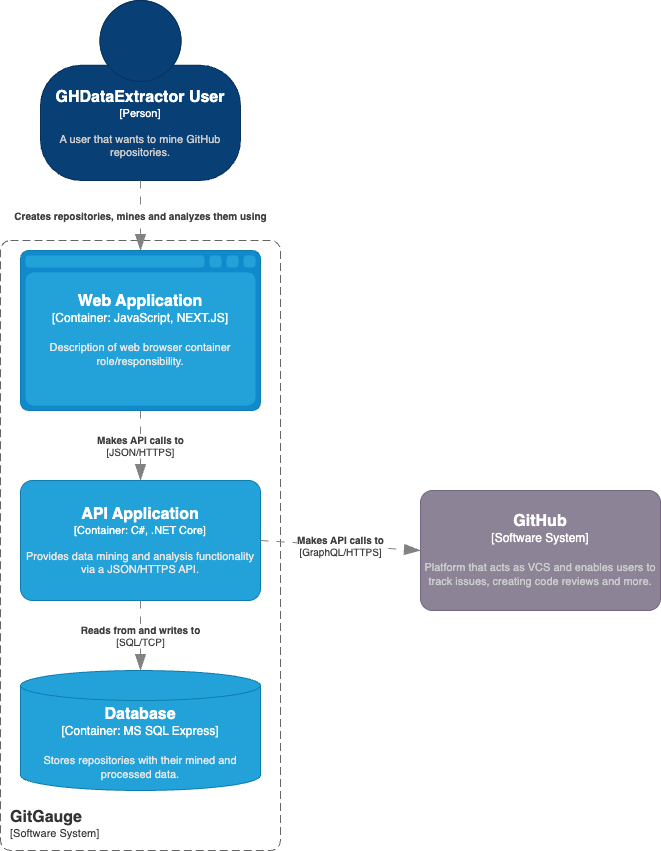
\includegraphics[width=0.8\textwidth]{Figures/container-diagram-gitgauge.png}
    \caption{Container-Diagramm GitGauge \parencite{grand_joel_vt1_joelgrand_repository_2024}}
    \label{fig:container-diagram-gitgauge}
\end{figure}

Das Frontend ist eine Next.js-Webapplikation. Die Benutzer können über die Oberfläche neue Repositories hinzufügen und anschliessend den Mining-Prozess starten. Der Mining-Prozess kann auch jederzeit wiederholt werden. Anschliessend werden alle verfügbaren Metriken dargestellt. Die Wahl fiel auf Next.js, da dies serverseitiges Rendering unterstützt. Dies verbessert die Performance und erleichtert das Fetching der Daten. \parencite{grand_joel_vt1_joelgrand_repository_2024}

Das Backend bietet eine REST-API, welche in C\# mithilfe von .NET Core implementiert wurde. Das Backend-Projekt ist in zwei Projekte unterteilt: dem Kernprojekt für die Hauptlogik und einem Data-Projekt, das als Object-Relational-Mapping (ORM) Schicht die Datenschemata definiert. Intern folgt das Backend einer geschichteten Architektur mit klar getrennten Verantwortlichkeiten. Von den Controller-Klassen (für die REST-API) über Services (Businesslogik) bis zur Datenzugriffsschicht (Data Store). \parencite{grand_joel_vt1_joelgrand_repository_2024}

Die Datenbank speichert sämtliche Daten, welche über die Projekte gesammelt wurden. Als Datenbank wird ein MSSQL-Server 2019 eingesetzt. \parencite{grand_joel_vt1_joelgrand_repository_2024}

\subsection{Repository Mining}
Das Mining der Daten wird in GitGauge mittels einer Mining-Pipeline abgebildet. Wie in \autoref{fig:overview-mining-steps} ersichtlich, besteht das Minen aus folgenden Phasen: Datenextraktion, Datenverarbeitung und Datenanalyse. 
In der Datenextraktionsphase werden alle relevanten Informationen aus dem GitHub-Repository ermittelt. Dabei werden 3 zentrale Datenquellen verwendet: Commits, Issues und PRs. Für das Analysieren der Commits wird mittels der Bibliothek LibGit2Sharp das Repository geklont. Dadurch können eventuelle API-Beschränkungen (Rate-Limits) reduziert oder umgangen werden. Die Issues und PRs werden über die GraphQL-API von GitHub abgefragt. Im Vergleich zur klassischen REST-API performte die GraphQL-API deutlich besser, auch schon bei kleineren Projekten.  

In der Verarbeitungsphase werden die rohen GitHub-Daten bereinigt, gefiltert und in ein Analyseschema überführt. So werden fehlende Werte substituiert und die Daten normalisiert. 
Die Analyse der Daten erfolgt jeweils bei Abfrage der Statistik-API-Endpunkte des Backends. 

\begin{figure}[htbp]
    \centering
    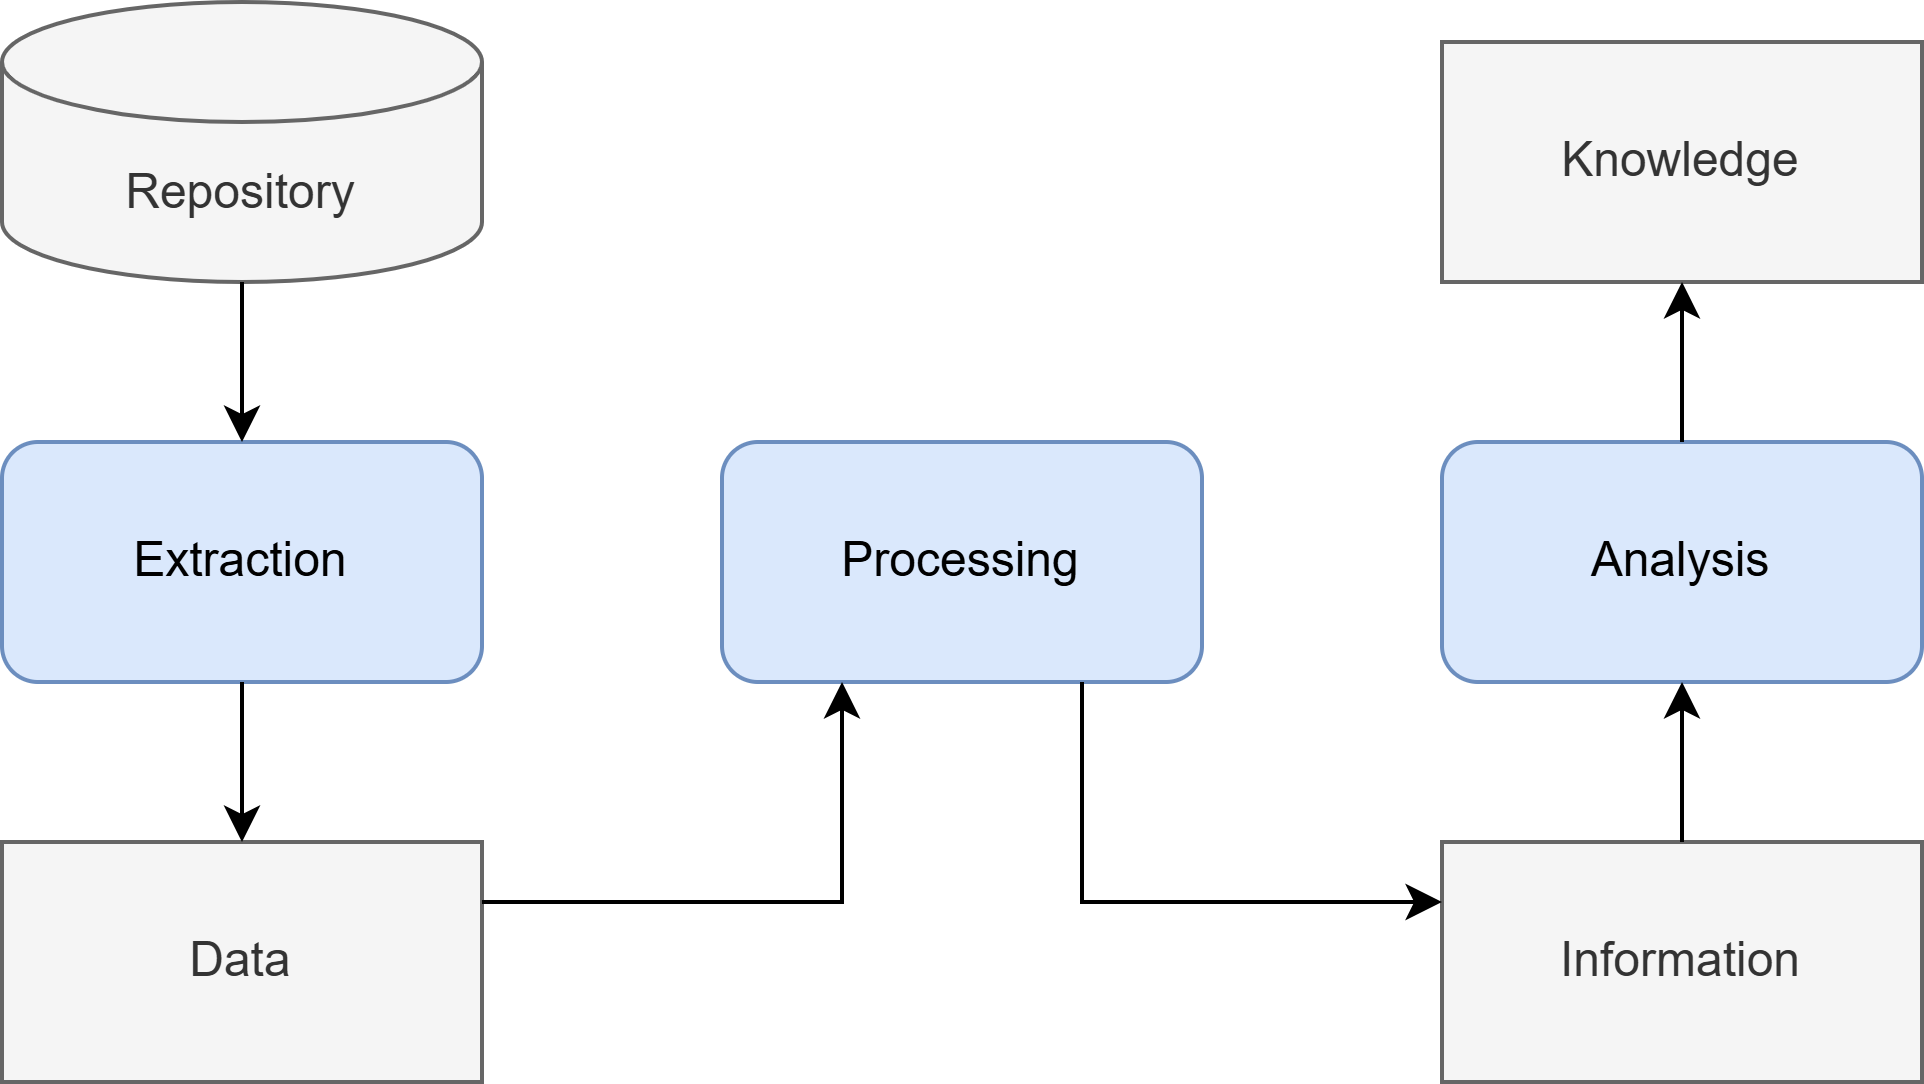
\includegraphics[width=0.8\textwidth]{Figures/uebersicht-mining-prozess.png}
    \caption{Übersicht Mining-Prozess \parencite{grand_joel_vt1_joelgrand_repository_2024}}
    \label{fig:overview-mining-steps}
\end{figure}

\pagebreak
 
% Indicate the main file. Must go at the beginning of the file.
% !TEX root = ../main.tex

%----------------------------------------------------------------------------------------
% CHAPTER TEMPLATE
%----------------------------------------------------------------------------------------


\chapter{Vorgehen / Methoden} % Main chapter title

\label{Chapter3} % Change X to a consecutive number; for referencing this chapter elsewhere, use \ref{ChapterX}

%----------------------------------------------------------------------------------------
% SECTION 1
%----------------------------------------------------------------------------------------

\section{Main Section 1}

Lorem ipsum dolor sit amet, consectetur adipiscing elit. Aliquam ultricies lacinia euismod. Nam tempus risus in dolor rhoncus in interdum enim tincidunt. Donec vel nunc neque. In condimentum ullamcorper quam non consequat. Fusce sagittis tempor feugiat. Fusce magna erat, molestie eu convallis ut, tempus sed arcu. Quisque molestie, ante a tincidunt ullamcorper, sapien enim dignissim lacus, in semper nibh erat lobortis purus. Integer dapibus ligula ac risus convallis pellentesque.

%-----------------------------------
% SUBSECTION 1
%-----------------------------------
\subsection{Subsection 1}

Nunc posuere quam at lectus tristique eu ultrices augue venenatis. Vestibulum ante ipsum primis in faucibus orci luctus et ultrices posuere cubilia Curae; Aliquam erat volutpat. Vivamus sodales tortor eget quam adipiscing in vulputate ante ullamcorper. Sed eros ante, lacinia et sollicitudin et, aliquam sit amet augue. In hac habitasse platea dictumst.

%-----------------------------------
% SUBSECTION 2
%-----------------------------------

\subsection{Subsection 2}
Morbi rutrum odio eget arcu adipiscing sodales. Aenean et purus a est pulvinar pellentesque. Cras in elit neque, quis varius elit. Phasellus fringilla, nibh eu tempus venenatis, dolor elit posuere quam, quis adipiscing urna leo nec orci. Sed nec nulla auctor odio aliquet consequat. Ut nec nulla in ante ullamcorper aliquam at sed dolor. Phasellus fermentum magna in augue gravida cursus. Cras sed pretium lorem. Pellentesque eget ornare odio. Proin accumsan, massa viverra cursus pharetra, ipsum nisi lobortis velit, a malesuada dolor lorem eu neque.

%----------------------------------------------------------------------------------------
% SECTION 2
%----------------------------------------------------------------------------------------

\section{Main Section 2}

Sed ullamcorper quam eu nisl interdum at interdum enim egestas. Aliquam placerat justo sed lectus lobortis ut porta nisl porttitor. Vestibulum mi dolor, lacinia molestie gravida at, tempus vitae ligula. Donec eget quam sapien, in viverra eros. Donec pellentesque justo a massa fringilla non vestibulum metus vestibulum. Vestibulum in orci quis felis tempor lacinia. Vivamus ornare ultrices facilisis. Ut hendrerit volutpat vulputate. Morbi condimentum venenatis augue, id porta ipsum vulputate in. Curabitur luctus tempus justo. Vestibulum risus lectus, adipiscing nec condimentum quis, condimentum nec nisl. Aliquam dictum sagittis velit sed iaculis. Morbi tristique augue sit amet nulla pulvinar id facilisis ligula mollis. Nam elit libero, tincidunt ut aliquam at, molestie in quam. Aenean rhoncus vehicula hendrerit.
% Indicate the main file. Must go at the beginning of the file.
% !TEX root = ../main.tex

%----------------------------------------------------------------------------------------
% CHAPTER TEMPLATE
%----------------------------------------------------------------------------------------


\chapter{Resultate} % Main chapter title

\label{Chapter4} % Change X to a consecutive number; for referencing this chapter elsewhere, use \ref{ChapterX}

%----------------------------------------------------------------------------------------
% SECTION 1
%----------------------------------------------------------------------------------------
In diesem Kapitel erfolgt eine Erläuterung der Resultate, die durch die Durchführung der oben beschriebenen Methoden erzielt werden. Dafür stehen, wie bereits im Kapitel \secref{sec:Datengrundlagen} erwähnt, 71 Repositories zur Verfügung. 

Des Weiteren sollen die folgenden Hypothesen anhand von Projekten der Studierenden untersucht werden.

\hypothese{hypothese1}{
Gegen Ende des Projekts werden Pull Requests schneller gemergt.
}

Die Projekte haben ein festes Ziel und einen festen Abgabetermin. Aus eigener Erfahrung der Autoren schieben Studierende gerne Arbeiten vor sich her und generieren dadurch mehr Arbeit für das Ende des Projektes. Aus diesem Grund gehen wir davon aus, dass Pull Requests gegen Ende des Projekts schneller bearbeitet werden.

\hypothese{hypothese2}{
Teilzeitstudierende nutzen Pull Requests effizienter als Vollzeitstudierende.

}


Wir gehen davon aus, dass Teilzeitstudierende durch ihre Arbeit mehr Erfahrung in der Durchführung von Softwareprojekten und somit auch in der Verwendung von Pull Requests haben. Dies kann sich in Anzahl, Grösse aber auch Kommentare unterscheiden. 


Für die ersten Experimente wurden die Repositories der Racetrack-Projekte ausgewertet. Wie im Kapitel \secref{sec:Projektmodule} erwähnt, findet dieses Projekt im Kontext des Projektmoduls 2 als erstes Projekt statt. Dieses dauert ungefähr vier Wochen, wobei die genaue Anzahl der Tage pro Klasse variieren kann. Das Grundgerüst des Sourcecodes wird in der Aufgabenstellung mitgeliefert, was die Vergleichbarkeit der Projekte erhöht. Ausserdem haben die Studenten schon Erfahrung mit der Handhabung von PullRequests. 

\newpage
\section{Churn vs Latency}
Zur Klärung der \fref{forschungsfrage1}: "\textit{Besteht ein Zusammenhang zwischen der Latency eines Pull
Requests (Zeit bis zum Merge oder Schliessung) und dem Churn (Anzahl geänderter Codezeilen) des jeweiligen Pull Requests?}" werden die geminten Repository Daten in einem Jupiter Notebook aufbereitet und graphisch dargestellt. Dazu werden die im Kapitel \secref{sec:Metriken} erwähnten Metriken \textit{createTime} und \textit{closeTime} gemined und damit die einzelnen Latencies berechnet. Um die Latency-Daten besser vergleichen zu können, werden diese noch vom Datumsformat in Stunden umgerechnet. Des Weiteren werden die Metriken  \textit{additions} und  \textit{deleteions} aus den Pull Requests extrahiert, um den Churn zu berechnen.

\subsection{Datenanalyse}
Zum besseren Verständnis der \textit{latency}- und \textit{churn}- Werte wird zunächst eine allgemeine Analyse der Daten durchgeführt.
Die Analyse basiert auf 2435 extrahierten Pull Requests. Wovon im Durchschnitt 34.3 Pull Requests pro Repository erstellt werden. In der folgenden Tabelle werden die wichtigsten Kennzahlen aufgezeigt.


\begin{table}[htbp]
    \centering
    \caption{Kennzahlen zu \textit{Latency} und \textit{Churn}}
    \begin{tabular}{@{}lrr@{}}
        \toprule
        \textbf & \textbf{Latency (in Stunden)} & \textbf{Churn} \\
         \midrule
        Mittelwert & 18.6 & 278.2 \\
        Standardabweichung &  42.0  & 815.8 \\
        Minimum & 0.0008 & 0.0 \\
        1. Quartil (Q1) & 0.05 & 28.0 \\
        Median & 0.6 & 94.0 \\
        3. Quartil (Q3) &  16.4   & 251.0 \\
        Maximum & 416.3 & 17299.0 \\
        \bottomrule
    \end{tabular}
    \label{tab:deskriptive-kennzahlen}
\end{table}

Die Analyse zeigt, dass ein durchschnittlicher Pull Request eine Bearbeitungszeit von 18.6 Stunden hat, während der Median bei 0.6 Stunden liegt. Dies deutet darauf hin, dass die meisten Pull-Requests sehr schnell bearbeitet werden und nur wenige eine sehr lange Bearbeitungszeit haben. Das wird auch durch die Standardabweichung von 42 Stunden deutlich.

Ein ähnliches Bild zeigt sich beim Churn. Auch hier liegt der Mittelwert mit 278 Codezeilenänderungen höher und der Median bei nur 94 Änderungen. Die Standardabweichung zeigt ebenfalls eine grosse Streuung der Daten.

Diese Werte sind zusätzlich in den Boxplots in den Abbildungen \autoref{fig:boxplot-latency} und \autoref{fig:boxplot-churn} ersichtlich. 
In beiden Abbildungen ist der Box-Bereich auf der linken Seite kompakt und nahe bei Null. 
Die \autoref{fig:boxplot-latency} zeigt ebenfalls, dass viele Pull Requests schnell abgearbeitet werden, während wenige längere Bearbeitungszeiten aufweisen. Es zeigt ausserdem auf, dass es eine Reihe von Ausreissern gibt. Diese belaufen sich auf 14\,\% aller \textit{latencies}.

\begin{figure}[htbp]
    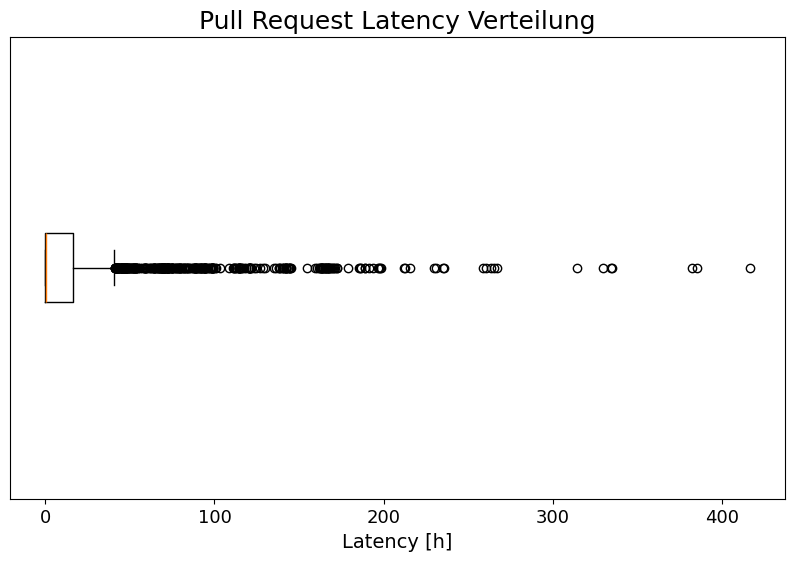
\includegraphics[width=0.8\textwidth]{Figures/boxplot-latency.png}
    \centering
    \caption{Boxplot Latency}
    \label{fig:boxplot-latency}
\end{figure}
 \newpage
Der Boxplot in der \autoref{fig:boxplot-churn} zeigt, dass es viele kleine Pull Requests mit wenigen Codezeilenänderungen gibt. Wie bereits bei der \textit{latency} wurde festgestellt, dass es eine Reihe von Ausreissern gibt, von denen einige besonders hervorstechen. Diese befinden sich bei über 10'000 Zeilenänderungen. In diesem Fall liegt die Anzahl der Ausreisser bei 9.6\,\%.

\begin{figure}[htbp]
    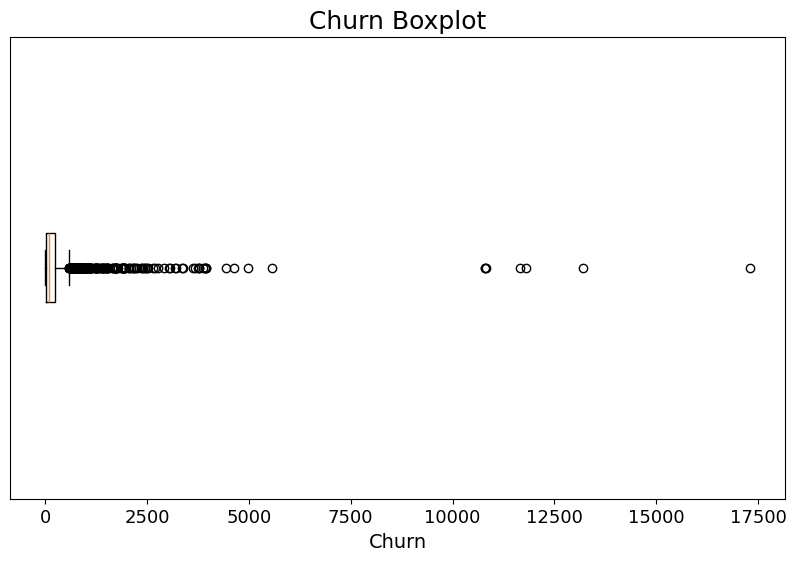
\includegraphics[width=0.8\textwidth]{Figures/boxplot-churn.png}
      \centering
    \caption{Boxplot Churn}
    \label{fig:boxplot-churn}
\end{figure}
\newpage
Werden die Ausreisser beider Metriken kumulativ aus allen Datensätzen herausgefiltert, bleiben 1887 Pull Requests übrig, was 77.5\,\% entspricht. Das Herausfiltern dieser Daten stellt einen erheblichen Eingriff in die Datenbasis dar und wird daher nicht pauschal vorgenommen.

\subsection{Ergebnisse}
Um festzustellen, ob zwischen den Metriken \textit{latency} und \textit{churn} ein Zusammenhang besteht wird die Spearman Rangkorrelation angewendet. Dafür wird die oben erwähnte \autoref{eqn:spearman} verwendet. Diese wird anhand der Phython Library \textit{pandas} berechnet. Als Ergebnis erreichte der Rangkorrelationskoeffizient einen Wert von 0.17. Dieser Wert liegt sehr Nahe bei null und zeigt somit keinen spezifischen Zusammenhang zwischen den beiden Metriken auf. 

Wie bereits erwähnt, weisen die Daten einen hohen Anteil an Ausreissern auf. Deshalb soll überprüft werden, ob die Metriken eine Korrelation besitzen, wenn diese Ausreisser herausgefiltert werden. In diesem Fall erhöht sich der Koeffizient auf 0.2, zeigt aber weiterhin keinen eindeutigen Zusammenhang zwischen den Metriken.

\textbf{Zusammenfassend kann zur \fref{forschungsfrage1} festgestellt werden, dass die Metriken \textit{latency} und \textit{churn} keinen Zusammenhang aufweisen.}

\section{Hypothese 2: Teilzeitstudierende nutzen Pull Requests effizienter als Vollzeitstudierende}
Zur detaillierten Analyse der Hypothese erfolgt eine Aufteilung der Repository-Daten auf Teilzeit- und Vollzeitklassen. Die Anzahl der Pull Requests der Teilzeitklassen beläuft sich auf 1369 und jene der Vollzeitklassen auf 1066. Dabei werden durchschnittlich 31.8 Pull Requests von den Teilzeitstudierenden erstellt und 39.5 von den Vollzeitstudierenden. In der folgenden Tabelle werden die wichtigsten Kennzahlen aufgezeigt.

\begin{table}[htbp]
    \centering
    \caption{Kennzahlen zu \textit{Latency} und \textit{Churn} von Teilzeit- und Vollzeitklassen}
    \begin{tabular}{@{}lrrrr@{}}
        \toprule
        \makecell{}&
        \makecell{\textbf{Latency (Std.)} \\ \textbf{Teilzeit}}&
        \makecell{\textbf{Latency (Std.)} \\ \textbf{Vollzeit}}&
        \makecell{\textbf{Churn} \\ \textbf{Teilzeit}}&
        \makecell{\textbf{Churn} \\ \textbf{Vollzeit}}\\
        \midrule
        Mittelwert & 19.9 & 16.9 & 260.2 & 301.3 \\
        Standardabweichung &  47.2 & 34.2  & 678.1 & 964.1 \\
        Minimum & 0.0008 & 0.001 & 0.0 & 0.0 \\
        1. Quartil (Q1) & 0.04 & 0.07 & 27.0 & 28.3\\
        Median & 0.5 & 0.8 & 93.0 & 97.0 \\
        3. Quartil (Q3) &  15.1 & 17.5 & 249.0 & 254.5 \\
        Maximum & 416.3 & 265.0 & 13206.0 & 17299.0 \\
        \bottomrule
    \end{tabular}
    \label{tab:deskriptive-kennzahlen-teilzeit-vollzeit}
\end{table}

Die \textit{latency} zeigt, dass Teilzeitstudierende im Durchschnitt mehr Zeit benötigen, um eine Pr zu bearbeiten. Der Median zeigt jedoch, dass die Teilzeitstudierenden mehr sehr kleine Pull Requests haben. Wobei bei beiden die Bearbeitungszeit im Median deutlich kürzer ist. Man sieht auch, dass die Teilzeitstudierenden eine grössere Streuung der Bearbeitungszeiten haben. Sie haben also gewisse Pull Requests die deutlich länger dauern. Dies ist auch im Maximum zu sehen, welches bei den Teilzeitstudierenden bei 416 Stunden liegt, was 17 Tagen entspricht. Wobei die Vollzeitstudierenden ein Maximum von 265 Stunden haben, was 11 Tagen entspricht.

Der \textit{churn} zeigt, dass Vollzeitstudierende sowohl im Durchschnitt als auch im Median mehr Zeilenänderungen pro Pull Request vornehmen. Die Standardabweichung zeigt ebenfalls, dass Vollzeitstudierende grössere Schwankungen in der Anzahl der Zeilenänderungen haben. Im Maximum ist ersichtlich, dass beide sehr grosse Prs haben, wobei sich das Maximum der Vollzeitstudierenden nochmals um mehr als 4'000 Zeilen unterscheidet.

Auch die Struktur der PRs unterscheidet sich leicht zwischen den Unterrichtsmodellen: Die durchschnittliche Anzahl bearbeiteter Dateien pro PR liegt insgesamt bei 5.66 Dateien. Teilzeitklassen weisen mit 5.85 im Schnitt mehr betroffene Dateien auf als Vollzeitklassen mit 5.42 Dateien. Ebenso zeigt sich bei der durchschnittlichen Anzahl Commits pro PR ein Unterschied: Insgesamt liegt der Durchschnitt bei 7.03 Commits pro PR, wobei Teilzeitklassen auf 6.50 und Vollzeitklassen auf 7.70 Commits pro PR kommen.

Um die Verteilung der \textit{latencies} zu analysieren, werden die Daten in Intervalle eingeteilt. Die Festlegung dieser Intervalle erfolgte auf der Grundlage bereits analysierter Daten. Nachfolgend eine Liste dieser Intervalle und die Gründe, warum sie so definiert wurden: 

\begin{itemize}
    \item \textbf{[0-1min]}: Für Pull Requests, die sofort gemerged werden.
    \item \textbf{[1-5min]}: Für Pull Requests, die schnell gemerged werden, bei denen aber noch genügend Zeit bleibt, sehr kleine Änderungen ernsthaft zu prüfen.
    \item \textbf{[5-30min]}: Für kleinere oder unkomplizierte Änderungen.
    \item \textbf{[0.5-1h]}: Um zu sehen, wie viele innerhalb einer Stunde abgeschlossen werden.
    \item \textbf{[1-4h]}: Diese Abgrenzung wurde gewählt, da 4 Stunden einen halben Arbeitstag / Studientag widerspiegeln, zum Beispiel auch die 4 Lektionen für die Projektmodul-Vorlesung.
    \item \textbf{[4-12h]}: 12 Stunden wurden gewählt, da dies einen halben Tag widerspiegelt, zum Beispiel wenn jemand morgens einen Pull Request eröffnet und ein Teammitglied abends Zeit hat, diesen zu bearbeiten.
    \item \textbf{[12-24h]}: Für alle Pull Requests, die innerhalb eines Tages gemerged werden.
    \item \textbf{[1-2d]}: Für alle Pull Requests, die mit einem Tag Verzögerung gemerged werden.
    \item \textbf{[2-7d]}: Um zu sehen, wie viele Pull Requests in derselben Woche noch bearbeitet werden.
    \item \textbf{[7d+]}: Für alle Pull Requests, die länger als eine Woche offen sind.
\end{itemize}


Die \autoref{fig:anz-prs-vs-latency-tv} zeigt die Pull Requests der Vollzeit- und Teilzeitklassen aufgeteilt in die oben genannten Intervalle. Es ist ersichtlich, dass ein Grossteil der Pull Requests in beiden Unterrichtsmodellen in den ersten drei Intervallen bearbeitet wurde. Im Intervall [0-1min] heben sich die Klassen der Teilzeitstudierenden jedoch stark ab. 
Die mittleren Latenzzeiten von einer halben Stunde bis zu einem Tag sind deutlich geringer. Bei den Unterrichtsmodellen gibt es keine nennenswerten Unterschiede. Lediglich bei den Bearbeitungszeiten von einer bis vier Stunden fallen die Teilzeitstudierenden auf. Auch die Bearbeitungszeiten von einem Tag bis zu einer Woche sind noch gut vertreten. Bei mehr als sieben Tagen heben sich die Teilzeitstudierenden wieder deutlich von den Vollzeitstudierenden ab.

\begin{figure}[htbp]
    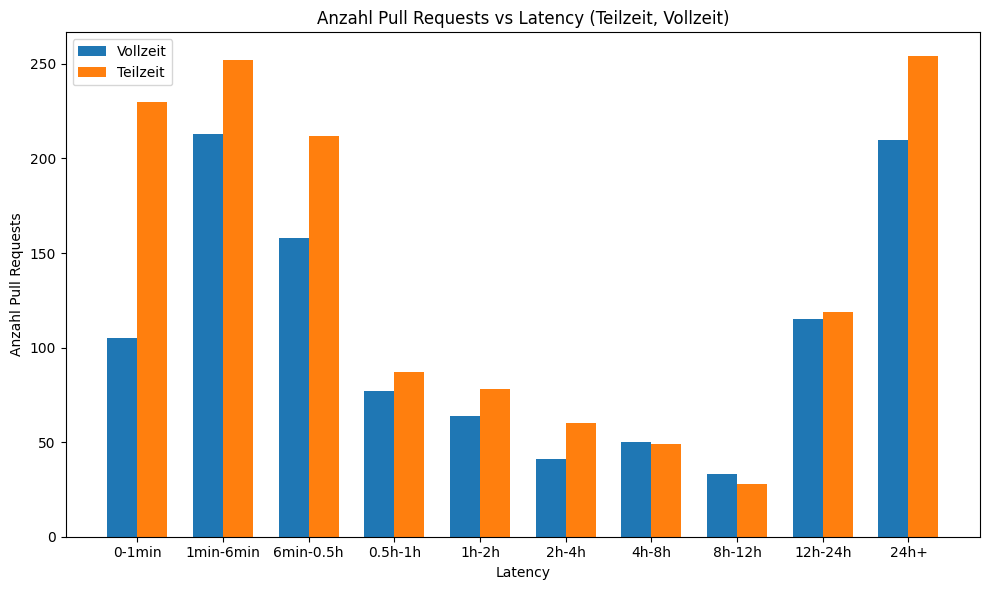
\includegraphics[width=\textwidth]{Figures/anz-prs-vs-latency-tv.png}
    \caption{Anzahl Pull Requests vs. Latency (Teilzeit, Vollzeit)}
    \label{fig:anz-prs-vs-latency-tv}
\end{figure}

Da in der Datenbasis mehr Teilzeitklassen und somit mehr Repositories vorhanden sind, werden die Daten auf die Anzahl der Repositories normiert, was eine unabhängigere Analyse ermöglicht.

Die \autoref{fig:anz-avg-prs-vs-latency-tv} zeigt nun, dass die Teilzeitstudierenden zwar immer noch viele Pull Requests innerhalb einer halben Stunde bearbeiten, aber nur im ersten Segment die Vollzeitstudierenden übertreffen. In den mittleren Intervallen sind die Teilzeitstudierenden relativ ausgeglichen, aber deutlich weniger als in den ersten drei Intervallen. Bei den Bearbeitungszeiten von mehr als sieben Tagen sind sie jedoch wieder stärker vertreten. Die Vollzeitstudierenden sind über alle Intervalle ausgeglichener, haben aber auch viele schnell bearbeiteten Pull Requests.


\begin{figure}[htbp]
    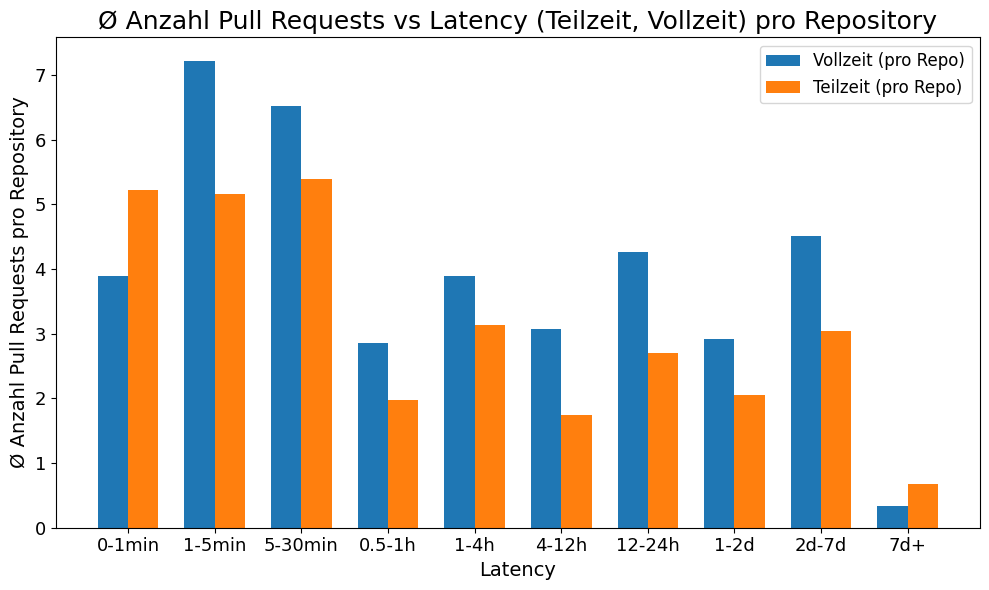
\includegraphics[width=\textwidth]{Figures/anz-avg-prs-vs-latency-tv.png}
    \caption{Durchschnittliche Anzahl Pull Requests vs. Latency (Teilzeit, Vollzeit)}
    \label{fig:anz-avg-prs-vs-latency-tv}
\end{figure}
\newpage
Insgesamt bestätigen die Abbildungen \autoref{fig:anz-prs-vs-latency-tv} und \autoref{fig:anz-avg-prs-vs-latency-tv}, dass die meisten Pull Requests schnell bearbeitet werden. Des Weiteren zeigt es, dass die Teilzeitstudierenden eine stärkere Streuung aufweisen als Vollzeitstudierende, da sie die Vollzeitstudierenden im ersten und letzten Intervall übertreffen.

// TODO Churn Latency
\newpage
Zur Klassifikation der Churn Grösse werden die von Doğan und Tüzün vorgeschlagenen Grössenkateogrien (XS, S, M, L, XL) verwendet. Diese Einteilung basiert auf empirischen Studien und industriellen Standards. \parencite{dogan_towards_2022}

Während der manuellen Untersuchung für die \fref{forschungsfrage2} wurde festgestellt, dass einige PRs einen Churn über 10'000 aufweisen. Entweder handelt es sich hierbei um geschlossene PRs welche entweder ausversehen erstellt oder beispielsweise mit dem falschen Zielbranch erstellt werden. Um diese zusätzlich klassifizieren zu können, wurde eine zusätzliche Grösse \textit{XXL} mit Churn \textit{10'000} erstellt. 

Somit ergibt sich für die Analyse folgende Klassifizierung: 
\begin{table}[ht]
\caption{Churn Grössenkategorien}
\label{tab:churnkategorien}
\centering
\begin{tabular}{l l}
\toprule
\textbf{Kategorie} & \textbf{Churn} \\
\midrule
XS  & 0--9       \\
S        & 10--49     \\
M        & 50--199    \\
L         & 200--999   \\
XL   & 1000--9999 \\
XXL  & 10000+ \\
\bottomrule
\end{tabular}
\end{table}


Abbildung \autoref{fig:anz-prs-vs-churn-size-tz-vz} zeigt die Pull Request der Voll- und Teilzeitklassen aufgeteilt nach ihrer Churn Grösse. So ist sichtbar, dass die Teilzeitklassen insegsamt mehr PRs erstellen. Dieser Trend ist in allen Grössenaktegorien sichtbar, ausser bei den \textit{XXL} PRs. Hier verfügen die Teilzeitklassen ingesamt über 2 PRs, während die Teilzeitklassen 5 PRs mit einem Churn über 10'000 verfügen. Bei den \textit{XXS} PRs verfügen die Teilzeitklassen über 1.5x so viele PRs.

\begin{figure}[htbp]
    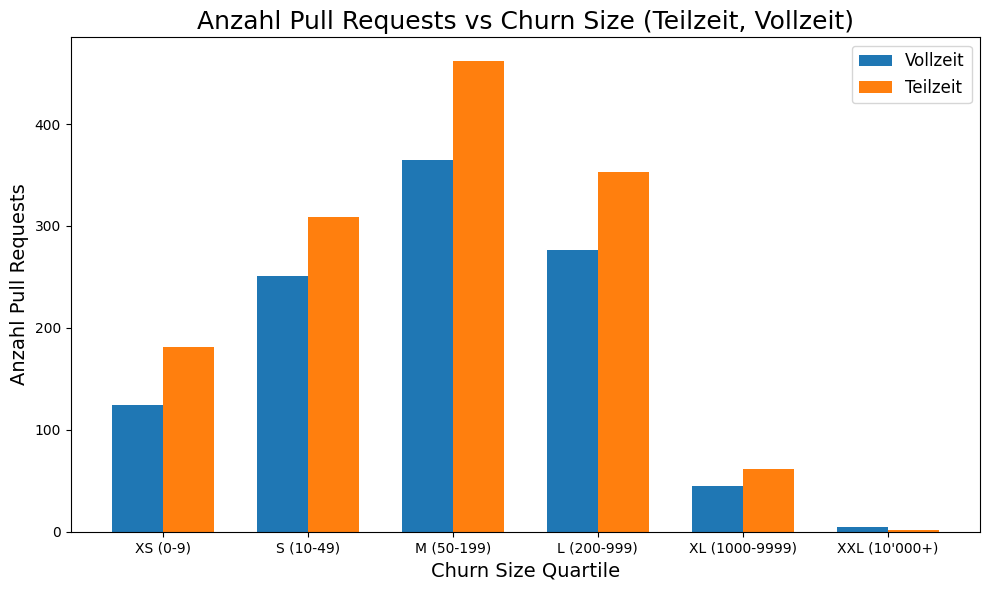
\includegraphics[width=\textwidth]{Figures/anz-prs-vs-churn-size-tz-vz.png}
    \caption{Anzahl PullRequests vs. Churn Grösse (Teilzeit, Vollzeit)}
    \label{fig:anz-prs-vs-churn-size-tz-vz}
\end{figure}

Eine Normalisierung der Daten, welche nun die durchschnittliche Anzahl PRs pro Repo zeigt, dass die Vollzeitklassen entweder gleich viel oder mehr PRs pro Kategorie erstellen. Die Teilzeitklassen erstellen jedoch fast gleich viele PRs in den Kategorien \textit{XS} und \textit{XL}, dort erstellen die Vollzeitklassen jeweils 1,12 und 1,18 so viele PRs. 

\begin{figure}[htbp]
    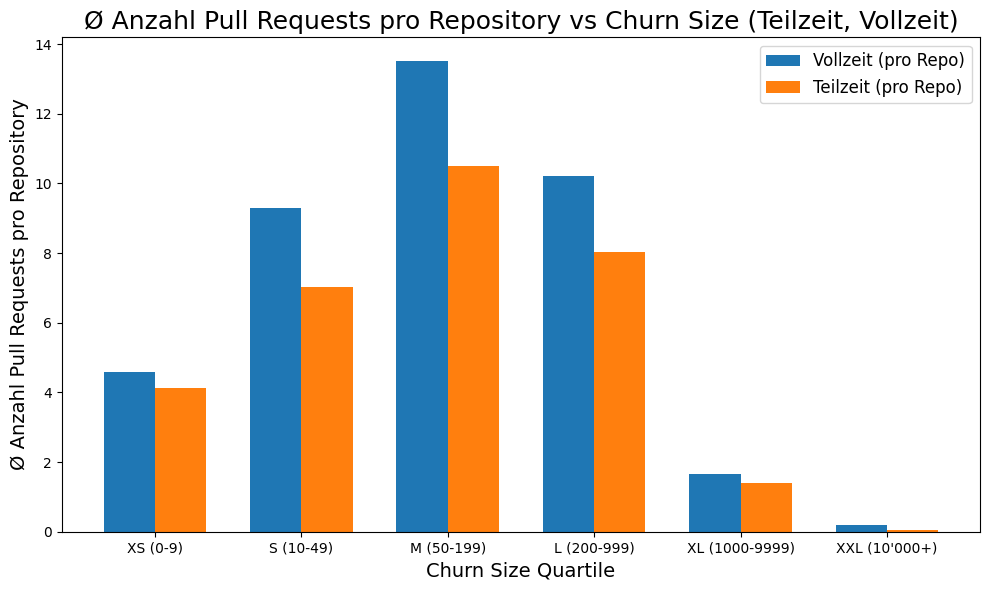
\includegraphics[width=\textwidth]{Figures/avg-anz-prs-vs-churn-size-tz-vz-pro-repo.png}
    \caption{Durchschnittliche Anzahl PullRequests vs. Churn Grösse pro Projekt(Teilzeit, Vollzeit)}
    \label{fig:anz-prs-vs-churn-size-tz-vz}
\end{figure}

Die für die \fref{forschungsfrage2} benötigte manuelle Untersuchung ergab, dass in einigen Klassen das in Kapitel \secref{sec:GitFlow} eingeführte Branching Konzept \textit{Git Flow} verwendet haben. Dies verfälscht eventuell die Daten, da es sich bei den manuell untersuchten Pull Requests um grosse PRs (Churn) handelt, welche keinen Review erfordern. Aus diesem Grund, werden die Analysen erneut durchgeführt jedoch mit herausgefilterten Dev Branches.

Da die Namen der Dev-Branches nicht einheitlich sind, werden alle Branches herausgefiltert, die das Wort Dev enthalten und auf den Main/Master Branch gemerged werden. Dabei ist zu beachten, dass GitHub den heutigen Haupt-Branch Main nennt, während dieser früher Master hiess. In der manuellen Analyse wurde festgestellt, dass einige Klassen aus dem Jahr 2021 immer noch solche Master Branches verwenden. Zusätzlich wurden alle herausgefilterten Pull Requests überprüft, um sicherzustellen, dass ausschliesslich Dev-Branches entfernt werden. Es wurden 75 Pull Requests von Dev-Branches zu Main-Branches ermittelt.


%// TODO anpassen wenn überhaupt beide grafiken
% Die Entfernung der Datensätze, welche Merges zwischen Developer-Branches und Main-Branches abbilden, verändert die Resultate marginal. Dies ist in der \autoref{fig:anz-prs-vs-latency-tv-no-dev} ersichtlich. Ebenso überwiegen in den ersten drei Spaltenpaaren und im letzten Paar die Teilzeitklassen. Am auffälligsten ist wiederum das erste Säulenpaar. Hier beträgt der Anteil der Teilzeitstudierenden an der Gesamtzahl der Teilzeitstudierenden 16 Prozent und bei den Vollzeitklassen 9.3 Prozent. Die Anzahl der Pull-Requests, die in weniger als einer Minute bearbeitet werden, ist also in beiden Klassen zurückgegangen, liegt aber in beiden Fällen unter einem Prozent.
% Addiert man die ersten drei Säulenpaare, so ergibt sich für die Teilzeitklassen ein Wert von 49.7 Prozent und für die Vollzeitklassen ein Wert von 43.3 Prozent. Damit liegen die Werte für die Teilzeit um genau ein Prozent und für die Vollzeit um 1.4 Prozent niedriger. Bei den 24 Stunden plus beträgt der Wert bei den Teilzeitklassen 19 Prozent, was einer Differenz von 0.4 Prozent entspricht. Bei den Vollzeitklassen beträgt der Wert 20.2 Prozent, was einem Anstieg von 0.5 Prozent gleichkommt.

% \begin{figure}[htbp]
%     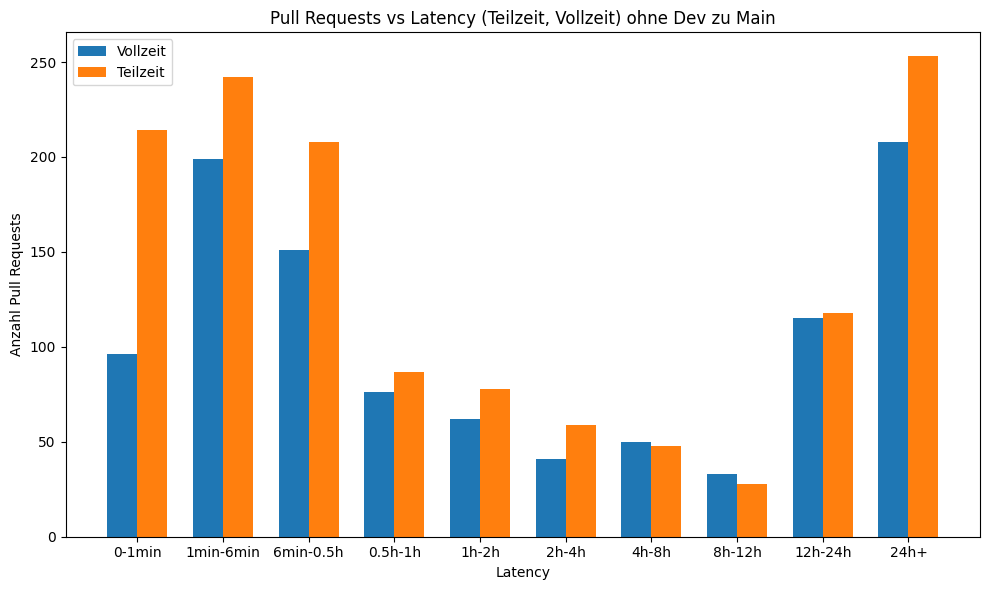
\includegraphics[width=\textwidth]{Figures/anz-prs-vs-latency-tv-no-dev.png}
%     \caption{Anzahl PullRequests vs. Latency (Teilzeit, Vollzeit) ohne Dev zu Main}
%     \label{fig:anz-prs-vs-latency-tv-no-dev}
% \end{figure}

Die \autoref{fig:anz-avg-prs-vs-latency-tv-no-dev} zeigt kaum Differenzen zur \autoref{fig:anz-avg-prs-vs-latency-tv}. Generell hat die durchschnittliche Anzahl der Pull Requests abgenommen, aber die Verteilung der Pull Requests unabhängig vom Unterrichtsmodell hat sich kaum verändert. 

\begin{figure}[htbp]
    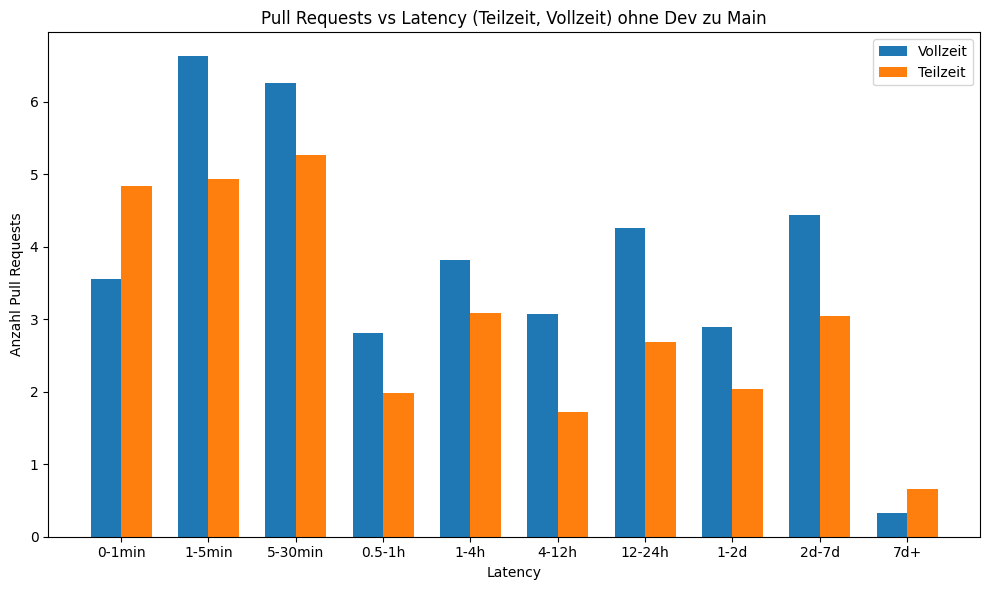
\includegraphics[width=\textwidth]{Figures/anz-avg-prs-vs-latency-tv-no-dev.png}
    \caption{Durchschnittliche Anzahl Pull Requests vs. Latency (Teilzeit, Vollzeit) ohne Dev zu Main}
    \label{fig:anz-avg-prs-vs-latency-tv-no-dev}
\end{figure}
\newpage

Nach der Entfernung der Pull Requests, die von Dev-Branches auf Main- oder Master-Branches gemerged wurden, bleibt das Bild in Bezug auf die Churn-Grössen weitgehend unverändert.

Abbildung \autoref{fig:anz-prs-vs-churn-size-tz-vz-ohne-dev} zeigt die durchschnittliche Anzahl von Pull Requests pro Repository, diesmal unter Einbeziehung der Dev-Branch-Merges. Es ist ersichtlich, dass die Vollzeitklassen in allen Churn-Kategorien tendenziell mehr Pull Requests pro Repository erstellen als die Teilzeitklassen. Besonders in den Kategorien \textit{M} (50–199 Änderungen) und \textit{L} (200–999 Änderungen) ist der Unterschied deutlich ausgeprägt. In den Kategorien \textit{XS} (0–9 Änderungen) und \textit{S} (10–49 Änderungen) ist der Abstand zwischen Teilzeit- und Vollzeitklassen zwar etwas geringer, aber immer noch zugunsten der Vollzeitklassen.

\begin{figure}[htbp]
    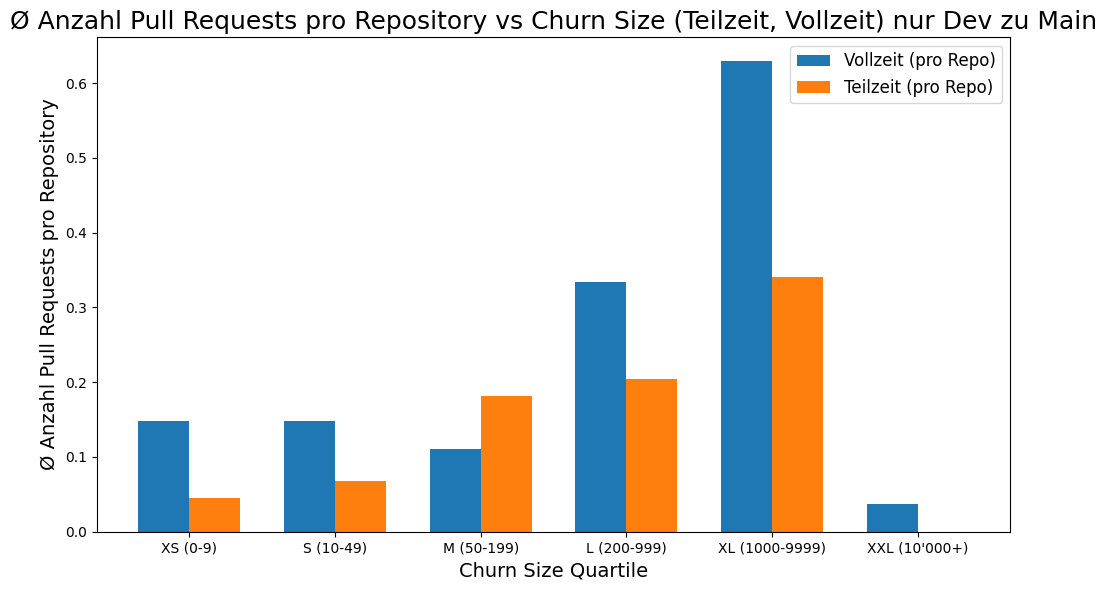
\includegraphics[width=\textwidth]{Figures/avg-anz-prs-vs-churn-size-tz-vz-pro-repo-ohne-dev.png}
    \caption{Durchschnittliche Anzahl PullRequests vs. Churn Grösse pro Projekt(Teilzeit, Vollzeit) ohne Dev zu Main}
    \label{fig:anz-prs-vs-churn-size-tz-vz-ohne-dev}
\end{figure}

Zum Vergleich zeigt die Abbildung \autoref{fig:anz-prs-vs-churn-size-tz-vz-nur-dev} nur die PRs, die von Dev-Branches auf Main-Branches gemerged wurden. Hier zeigt sich, dass diese Pull Requests insbesondere in den grösseren Churn-Kategorien (\textit{L} bis \textit{XXL}) auftreten. Auffällig ist zudem, dass in dieser Betrachtung die Vollzeitstudierenden mehr grosse Dev-Branch Pull Requests erzeugen als die Teilzeitstudierenden.

\begin{figure}[htbp]
    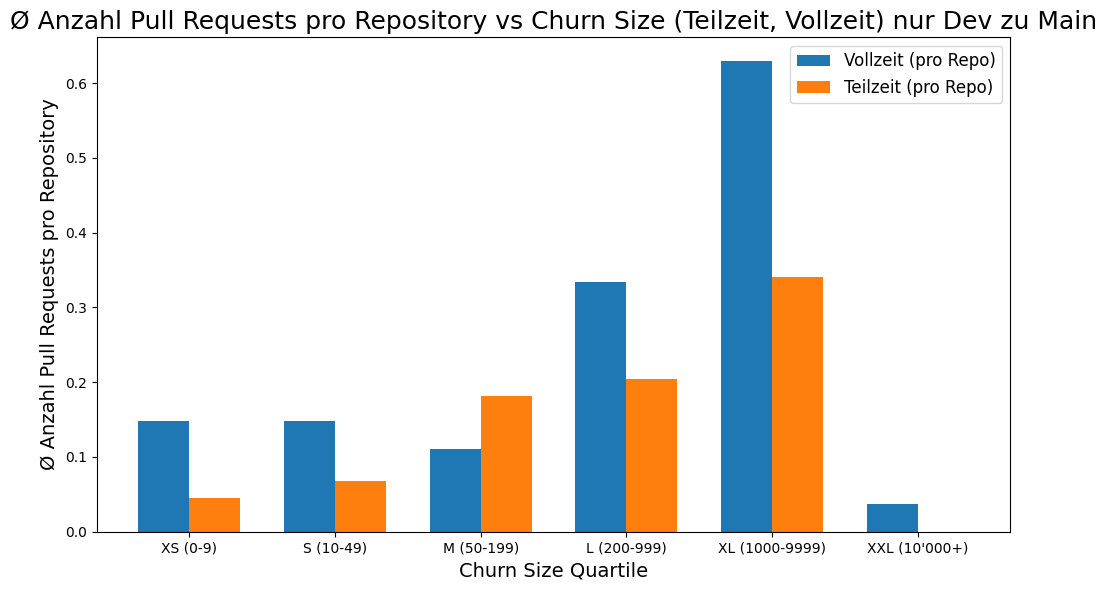
\includegraphics[width=\textwidth]{Figures/avg-anz-prs-vs-churn-size-tz-vz-pro-repo-nur-dev.png}
    \caption{Durchschnittliche Anzahl PullRequests vs. Churn Grösse pro Projekt(Teilzeit, Vollzeit) nur Dev zu Main}
    \label{fig:anz-prs-vs-churn-size-tz-vz-nur-dev}
\end{figure}

Zusammengefasst zeigt sich, dass die Herausfilterung der Dev-Branch-Merges einen Einfluss auf die Ergebnisse der Churn-Verteilung hat, insbesondere bei grossen Pull Requests. Insgesamt bestätigt sich jedoch, dass Vollzeitstudierende – unabhängig von der Herausfilterung – in den meisten Kategorien durchschnittlich mehr Pull Requests pro Repository erstellen als Teilzeitstudierende.

// TODO Abschluss kapitel

\section{Hypothese 1 Einfluss von Projektzeit}
Als nächstes wurde der Zusammenhang zwischen der laufenden Projektzeit und der \textit{latency} untersucht. Um zu ermitteln, ob die fortschreitende Projektzeit einen Einfluss auf das Bearbeiten der Pull Requests hat und um zu sehen, ob die \hyref{hypothese2} "\textit{Gegen Ende des Projekts werden Pull Requests schneller gemergt.}" zutrifft. Zusätzlich werden auch die \textit{churns} untersucht, um zu sehen, wie sich diese im Verlauf der Projektzeit verändern. 

Ein signifikanter Faktor, der bei den Projektmodulen eine Rolle spielt, ist der fest definierte Abgabetermin. Dies unterscheidet diese Projekte von Open-Source-Projekten, die in der Literatur häufig untersucht werden. Um diese Untersuchung durchführen zu können, wird zusätzlich zu den oben genannten Metriken der Abgabetermin der einzelnen Klassen ermittelt. Dazu wird für jede Klasse der zuletzt erstellte Pull Request gezogen. Da einige Dozierende ihr Feedback per Pull Request abgeben, werden alle Pull Requests eines Dozierenden herausgefiltert. Dies wird über das Attribut \textit{Author} ermittelt. Die Verifizierung dieser Methode erfolgte unter Zuhilfenahme der bekannten <nr> Abgabetermine von Klassen.

Zur initialen Analyse werden die Projekte in die entsprechenden Projektwochen aufgeteilt und die Mediane der \textit{latenncies} und \textit{churns} der entsprechenden Wochen ermittelt. Dies soll eine allgemeine Übersicht der Veränderungen der Metriken aufzeigen.

\subsection{Projektwochen im Verhältnis zu Latency und Churn}
\label{sec:ProjektwochenLatencyChurn}
In welcher Woche ein Pull Request stattfindet wird ermittelt indem die im Kapitel \secref{sec:Metriken} erwähnten Metriken \textit{Pull Request createTime} und \textit{Repository createTime} gemined werden und die Erstellungszeit des Repositroies abgezogen wird von der Eröffnungszeit des Pull Requests. 


Anhand der \autoref{fig:mittelwert-woche-lateny} ist ersichtlich, dass die Latency gegen Ende der Projektzeit abnimmt, während die Churn (\autoref{fig:mittelwert-woche-churn}) bis zur 5. Woche ansteigt. 
Zu beachten ist, dass, wie bereits im Kapitel \secref{sec:Projektmodule} erwähnt, die Projekte nicht exakt 28 Tage dauern. Die ermittelten Projektlaufzeiten liegen zwischen 20 und 36 Tagen.
Wobei die Klassen aus den Jahren 2021 und 2022 bei einem Durchschnitt von 21 Tagen liegen. Die neueren Klassen ab dem Jahr 2023 haben eine Projektlaufzeitspannweite von 28 bis 36 Tagen, wobei eine Klasse 35 Tage überschreitet. In dieser Klasse haben fünf Teams eine Laufzeit von 29 Tagen und drei Teams eine Laufzeit von 35 oder 36 Tagen. Somit widerspiegeln diese drei Teams die Woche sechs in der folgenden \autoref{fig:vergleich-latency-churn-projektzeit}. Die Latency nimmt im Laufe der Zeit zweimal stark ab. Das erste Mal von der ersten zur zweiten Projektwoche, wobei sie in der ersten Woche bei einem Median von 3.5 Stunden und in der zweiten Woche bei 2 Stunden liegt. Zum zweiten Mal nimmt die Latenz in der vierten Projektwoche stark ab, und zwar von 1.7 Stunden auf 0.5 Stunden. In der sechsten Woche ist die Latency nahezu 0. Der Churn steigt bis zur 5. Woche kontinuierlich von 72 Zeilenwechseln auf 115 an und sinkt dann in der 6. Woche auf 98.
\begin{figure}[htbp]
    \centering
    \begin{subfigure}[b]{0.48\textwidth}
        \centering
        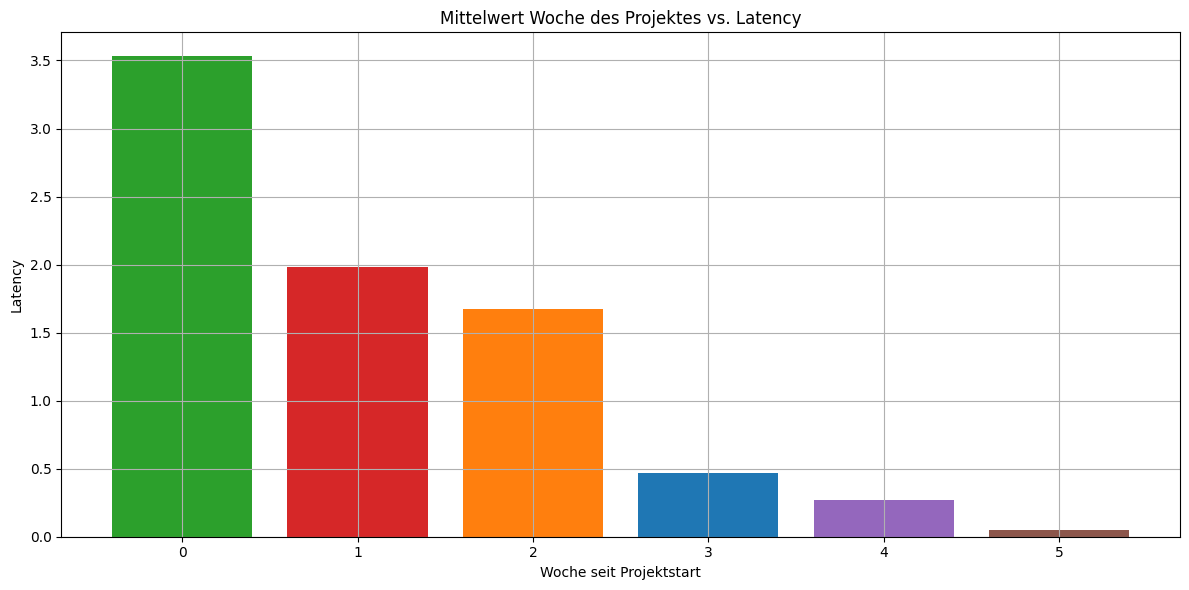
\includegraphics[width=\textwidth]{Figures/mittelwert-woche-lateny.png}
        \caption{Mediane Woche des Projektes vs. Latency}
        \label{fig:mittelwert-woche-lateny}
    \end{subfigure}
    \hfill
    \begin{subfigure}[b]{0.48\textwidth}
        \centering
        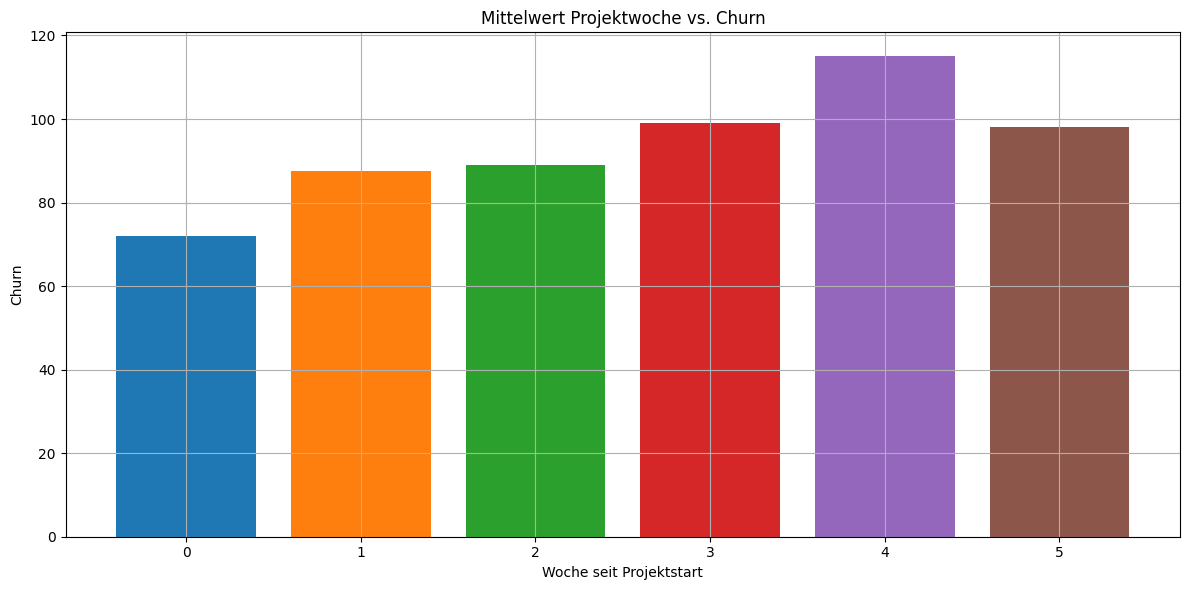
\includegraphics[width=\textwidth]{Figures/mittelwert-woche-churn.png}
        \caption{Mediane Woche des Projektes vs. Churn}
        \label{fig:mittelwert-woche-churn}
    \end{subfigure}
    \caption{Vergleich von Latency und Churn innerhalb der Projektzeit}
    \label{fig:vergleich-latency-churn-projektzeit}
\end{figure}

Werden die Daten nach Vollzeit- und Teilzeitstudierenden aufgeteilt, zeigt sich bei den Vollzeitklassen ein ähnliches Bild. Veranschaulicht wird dies in der \autoref{fig:vergleich-latency-churn-projektzeit-v}. Allerdings ist der Median der Latency in der ersten Woche mit 7.4 Stunden mehr als doppelt so hoch wie in der Gesamtauswertung. Ebenso nimmt die Latency von der ersten zur zweiten Woche stark ab. Der Wert sinkt um mehr als die Hälfte und liegt anschliessend bei 3.4 Stunden. Ab der vierten Woche ist der Median unter einer halben Stunde. Zeitgleich ist der Churn in der ersten Woche mit 71 Zeilenänderungen am geringsten, steigt mit Ausnahme der dritten Woche an und erreicht in der fünften Woche mit 121 Änderungen seinen Höhepunkt. Im Gegensatz zur Latency liegen diese Werte sehr nahe bei der Gesamtanalyse.
\begin{figure}[htbp]
    \centering
    \begin{subfigure}[b]{0.48\textwidth}
        \centering
        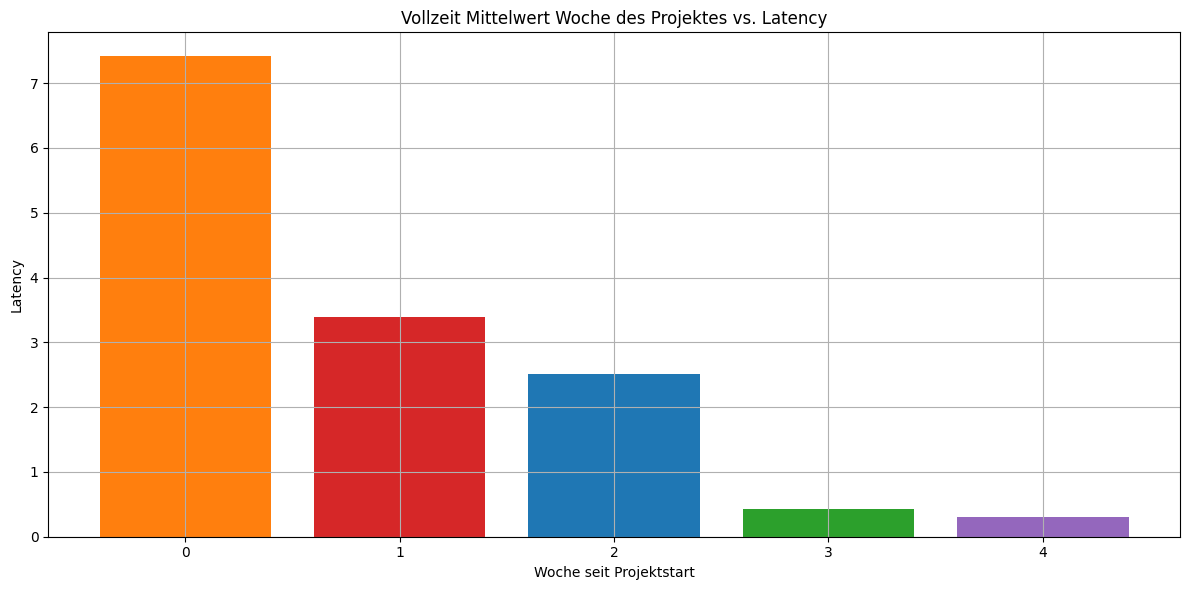
\includegraphics[width=\textwidth]{Figures/mittelwert-woche-lateny-v.png}
        \caption{Mediane Woche des Projektes vs. Latency Vollzeit}
        \label{fig:mittelwert-woche-lateny-v}
    \end{subfigure}
    \hfill
    \begin{subfigure}[b]{0.48\textwidth}
        \centering
        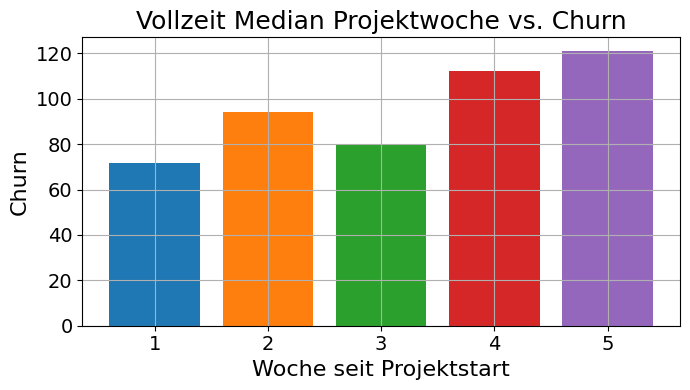
\includegraphics[width=\textwidth]{Figures/mittelwert-woche-churn-v.png}
        \caption{Mediane Woche des Projektes vs. Churn Vollzeit}
        \label{fig:mittelwert-woche-churn-v}
    \end{subfigure}
    \caption{Vergleich von Latency und Churn innerhalb der Projektzeit Vollzeit}
    \label{fig:vergleich-latency-churn-projektzeit-v}
\end{figure}

In der \autoref{fig:vergleich-latency-churn-projektzeit-t} ist zu erkennen, dass auch bei den Teilzeitstudierenden die Latency in der ersten Woche am höchsten ist, sich aber weniger stark von den Wochen zwei und drei unterscheidet. Zusätzlich ist der Wert der ersten Woche im Gegensatz zur Gesamtanalyse und vor allem den Vollzeitstudierenden tiefer bei einem Wert von knapp 2 Stunden. Zudem steigt bei den Teilzeitklassen in der dritten Woche die Latency nochmals an, aber dies nur mit einem Unterschied von 0.1 Stunden. Danach sinkt die Latency ebenso und liegt in Woche vier unter einer Stunde. Der Churn steigt ebenfalls an und erreicht in Woche fünf seinen Höhepunkt bei 110 Codezeilenänderungen. Die Werte der Churn befinden sich im gleichen Rahmen wie bei den Vollzeitstudierenden.

\begin{figure}[htbp]
    \centering
    \begin{subfigure}[b]{0.48\textwidth}
        \centering
        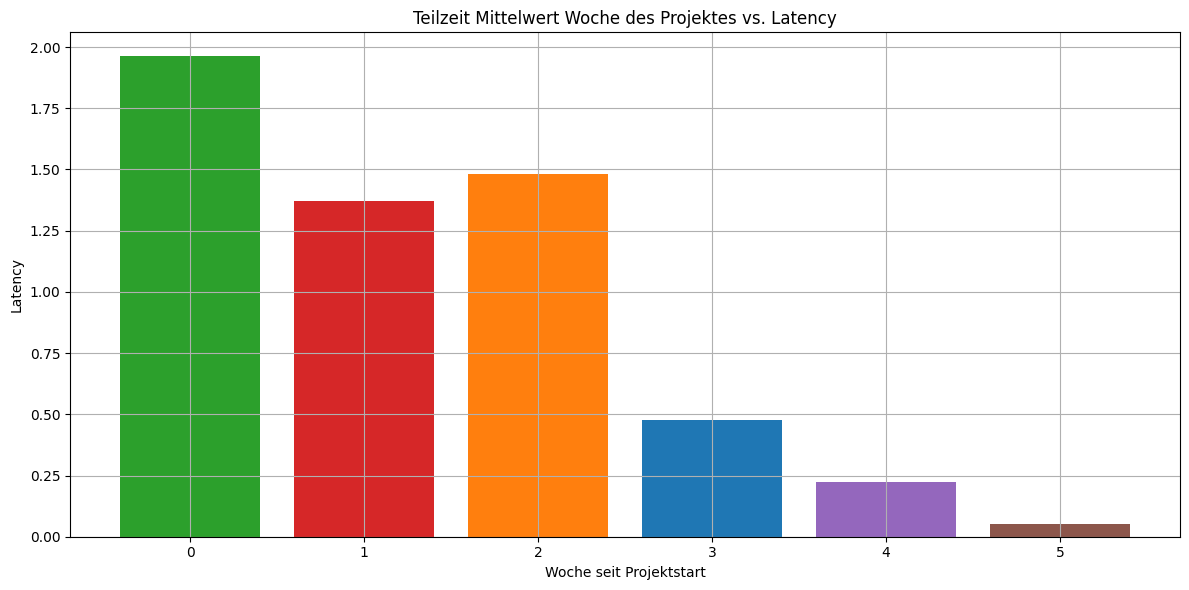
\includegraphics[width=\textwidth]{Figures/mittelwert-woche-lateny-t.png}
        \caption{Mediane Woche des Projektes vs. Latency Teilzeit}
        \label{fig:mittelwert-woche-lateny-t}
    \end{subfigure}
    \hfill
    \begin{subfigure}[b]{0.48\textwidth}
        \centering
        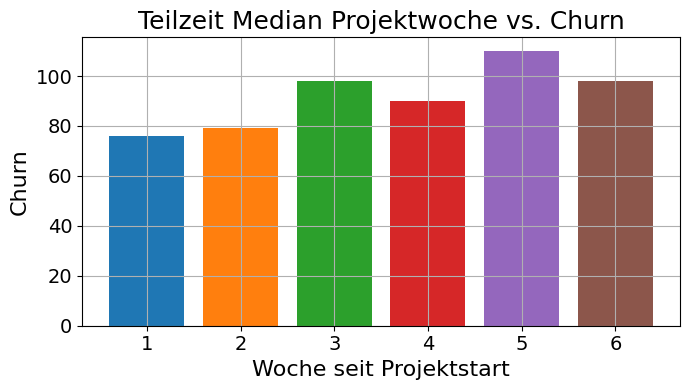
\includegraphics[width=\textwidth]{Figures/mittelwert-woche-churn-t.png}
        \caption{Mediane Woche des Projektes vs. Churn Teilzeit}
        \label{fig:mittelwert-woche-churn-t}
    \end{subfigure}
    \caption{Vergleich von Latency und Churn innerhalb der Projektzeit Teilzeit}
    \label{fig:vergleich-latency-churn-projektzeit-t}
\end{figure}
Zusammenfassend lässt sich feststellen, dass die Latency im Laufe der Zeit abnimmt, während der Churn zunimmt. Es ist auch ersichtlich, dass Vollzeitstudierende vor allem in der ersten Woche einen deutlich höheren Wert bei der Bearbeitungszeit der Pull Requests haben. Jedoch gilt zu beachten, dass wie bereits erwähnt, nicht alle Projekte gleich lange dauerten und somit waren bei den Wochen vier, fünf und sechs nicht mehr alle Projekte am laufen. Deshalb wurde ermittelt, wie die Pull Requests Verteilung über die Projektwochen ist.

\begin{table}[ht]
\caption{Anzahl Pull Requests pro Woche}
\label{tab:anz_pr_per_week}
\centering
\begin{tabular}{rrrr}
\toprule
\textbf{Woche} & \textbf{Vollzeit} & \textbf{Teilzeit} & \textbf{Gesamt} \\
\midrule
1 & 94 & 107 & 201 \\
2 & 158 & 174 & 332\\
3 & 275 & 317 & 592\\
4 & 298 & 363 & 661\\
5 & 241 & 341 & 582 \\
6 & 0 & 67 & 67\\
\bottomrule
\end{tabular}
\end{table}

\newpage
Wie in der \autoref{tab:anz_pr_per_week} ersichtlich wurden die wenigsten Pull Requests in der sechsten Woche erstellt. Zu diesem Zeitpunkt liefen jedoch nur noch drei Projekte. Abgesehen davon werden in der ersten Projektwoche die wenigsten Pull Requests erstellt. Diese Zahl steigt dann kontinuierlich bis zur 4. Woche an, obwohl in der 4. Woche nicht mehr alle Projekte am Laufen waren. In der fünften Woche ist ein Rückgang der Pull Requests zu beobachten, wobei diese in der Gesamtzahl nur geringfügig unter der dritten Woche und bei den Teilzeitstudierenden sogar leicht darüber liegt. 

Die Erstellung von Pull Requests ist in den letzten Wochen der Projekte sehr hoch. Allerdings ist nicht genau ersichtlich, wie sich die Pull Requests über die Laufzeit der einzelnen Projekte verteilen. Deshalb wird in einer weiteren Untersuchung analysiert, wie die Verteilung der Pull Requests im Verhältnis zu den Abgabefristen der einzelnen Projekte aussieht.

\subsection{Pull Requests im Verhältnis zum Abgabetermin}
Die Untersuchung von Pull Requests im Verhältnis zur Abgabe zeigt, dass am Tag der Abgabe die meisten Pull Requests abgearbeitet werden. Dies ist aus der \autoref{fig:anz-prs-days-away-from-end} ersichtlich. Von den 2427 untersuchten Pull Requests wurden 523 am Tag der Abgabe erstellt und abgeschlossen. Dieser Wert entspricht einer Quote von 21.5\,\%.  Die zweitmeisten Pull Requests wurden am Tag vor der Abgabe bearbeitet mit einer Anzahl von 309. Am drittletzten Tag wurde ein erhöhter Wert festgestellt, der jedoch nicht mehr signifikant hervorsticht. Eine Zusammenfassung der letzten drei Tage der Projekte ergibt eine Gesamtzahl von 986 bearbeiteten Pull Requests, was einem Prozentsatz von 40.6\,\% entspricht. Über die restliche Projektzeit variieren die Anzahl bearbeiteter Pull Requests. Es lassen sich erhöhte Werte sieben, acht und 15 Tage vor der Abgabe feststellen, die sich von den Werten der übrigen Tage abheben.
\begin{figure}[htbp]
    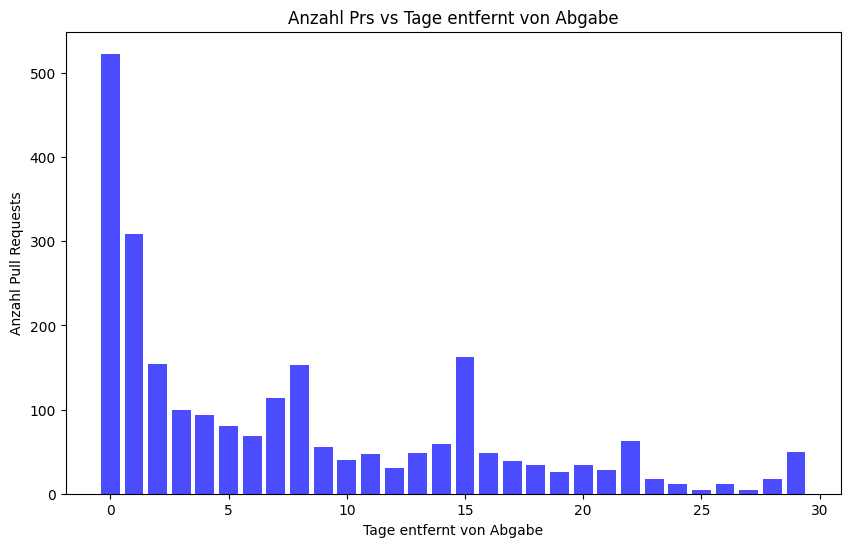
\includegraphics[width=\textwidth]{Figures/anz-prs-days-away-from-end.png}
    \caption{Anzahl eröffneter Pull Requests im Verhältnis zur Abgabe}
    \label{fig:anz-prs-days-away-from-end}
\end{figure}
\newpage
Eine detaillierte Analyse der Pull Requests in den einzelnen Teams zeigt, dass in 19 von 71 Teams mehr als 50 Prozent aller Pull Requests in den letzten drei Projekttagen eröffnet und abgeschlossen wurden. Es lässt sich feststellen, dass vier der analysierten Teams einen Anteil von über 75 Prozent ihrer Pull Requests in diesem Zeitraum bearbeitet haben. Zudem ist eine Gruppe zu identifizieren, die sämtliche ihrer Pull Requests innerhalb des definierten Zeitraums erstellt und geschlossen hat. Eine detaillierte Analyse des Projektes ergab, dass die genannte Gruppe insgesamt zwei Pull Requests hatte, die beide am Tag vor der Abgabe erstellt wurden. Wenn diese Analyse auf den letzten Projekttag beschränkt wird, dann sind es drei Teams, die mehr als 50 Prozent ihrer Pull Requests am Abgabetag erledigt haben.

Viele Pull Requests werden gegen Ende der Projekte erstellt und wie im Kapitel \secref{sec:ProjektwochenLatencyChurn} aufgezeigt, nehmen die Latencies gegen Ende der Projekte ab. Jedoch ist dort nicht genau ersichtlich, wie dies bei den einzelnen Projekten aussieht. Deshalb werden die Latencies unter 30 Minuten und die ganz kurzen Latencies von unter einer Minute im Verhältnis zu den Abgaben gestellt.

\newpage
\subsection{Analyse kurze Pull Request Latency im Verhältnis zur Abgabe }
Eine detaillierte Analyse der kurz geöffneten Pull Requests (kleiner als 30 Minuten) offenbart, dass der überwiegende Teil davon in den letzten drei Tagen und insbesondere am Tag der Abgabe erstellt werden. Eine weitere Restriktion der Pull Requests auf jene, die innerhalb einer Minute abgearbeitet werden, resultiert in einer ähnlichen Situation. Es ist jedoch festzustellen, dass der Tag der Abgabe sich stärker abhebt, wobei auch ein Anstieg zwei Tage vor Abgabe zu erkennen ist.  Die Resultate sind in \autoref{fig:anz-prs-under-x-mins} dargestellt.

\begin{figure}[htbp]
    \centering
    \begin{subfigure}[b]{0.48\textwidth}
        \centering
        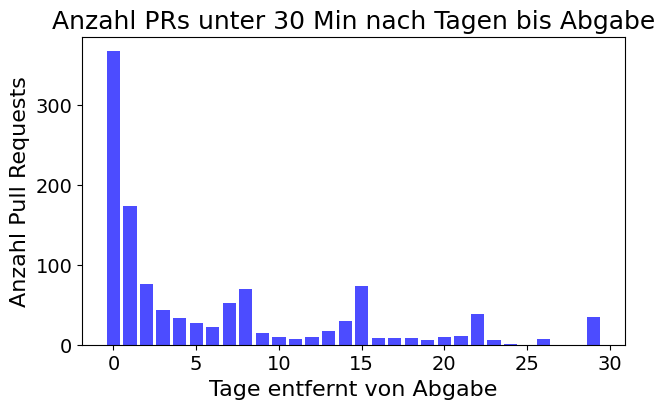
\includegraphics[width=\textwidth]{Figures/anz-prs-under-30-min.png}
    \caption{Anzahl Pull Requests unter 30 Minuten im Verhältnis zur Abgabe}
    \label{fig:anz-prs-under-30-min}
    \end{subfigure}
    \hfill
    \begin{subfigure}[b]{0.48\textwidth}
        \centering
        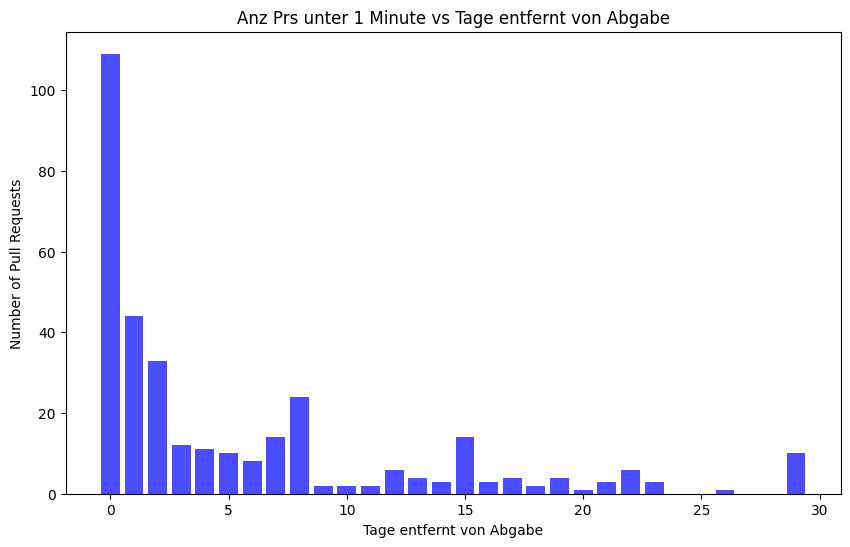
\includegraphics[width=\textwidth]{Figures/anz-prs-under-1-min.png}
    \caption{Anzahl Pull Requests unter einer Minute im Verhältnis zur Abgabe}
    \label{fig:anz-prs-under-1-min}
    \end{subfigure}
    \caption{Anzahl Pull Requests unter 30 / 1 Minute im Verhältnis zur Abgabe}
    \label{fig:anz-prs-under-x-mins}
\end{figure}


\newpage
\section{Ergebnisse Pull Reqeust Akzeptanz}
In diesem Abschnitt wird die Akzeptanz von PRs untersucht. Ziel ist es, die Gründe für die Ablehnung oder das Schliessen von PRs systematisch zu erfassen und mögliche Muster zwischen Vollzeit- und Teilzeitklassen herauszuarbeiten.

\subsection{Kategorisierung der geschlossenen Pull Requests}
\label{sec:KategorienGeschlossenePRs} 
// TODO: mit literatur vergleichen
Um die Ursache des geschlossenen PRs klassifizieren zu können, müssen zuerst Kategorien erstellt werden. Diese Kategorien wurden aufgrund einer manuellen Analyse des Datensatzes erreicht. Dabei wurden alle 39 PRs mit einem Churn von mindestens 500 manuell angeschaut als auch eine Stichprobe von 50 geschlossenen PRs mit einem kleinerem Churn.
\begin{itemize}
    \item \textbf{PRs ohne erkennbaren Grund (OG)}: Die PRs wurden ohne Kommentar geschlossen. Die Churn-Grösse ist kleiner als 500.
    \item \textbf{Feature durch anderen PR implementiert (FPI)}: Das Feature wurde durch einen anderen PR implementiert und der ursprüngliche PR anschliessend geschlossen.
    \item \textbf{PRs mit falschem Zielbranch (FZB)}: Der Autor des PRs wählte den falschen Zielbranch aus. Der PR wurde anschliessend in den korrekten Branch gemerged.
    \item \textbf{Feature wird nicht mehr benötigt (FNN)}: Das Feature wird nicht mehr benötigt. Dies muss explizit im PR vermerkt sein.
    \item \textbf{Implementierung abgelehnt (IA)}: Die vorgeschlagene Implementierung wurde abgelehnt.
    \item \textbf{Divers (DIV)}: Beinhaltet hauptsächlich Feedback-PRs, welche von gewissen Dozenten für die Notenvergabe verwendet wurden. Ausserdem sind einige Refactor-Branches zu sehen, welche ausschliesslich für den Refactoren erstellt wurden und anschliessend geschlossen wurden. 
\end{itemize}

\subsection{Deskriptive Analyse}
Insgesamt wurden 2427 Pull Requests untersucht, wovon 170 PRs geschlossen wurden (7,0,\%). Von den geschlossenen PRs entfielen 95 auf Vollzeitklassen und 75 auf Teilzeitklassen.

Der durchschnittliche Churn bei geschlossenen PRs beträgt: \begin{itemize} \item Teilzeitklassen: 137 Zeilenänderungen \item Vollzeitklassen: 188 Zeilenänderungen \end{itemize}

Eine Aufteilung der geschlossenen Pull Requests nach Churn-Grösse zeigt, dass in Teilzeitklassen vorwiegend kleinere PRs geschlossen wurden, während in Vollzeitklassen die Spannweite der Churn-Grössen etwas grösser ist.

\begin{figure}[htbp]
    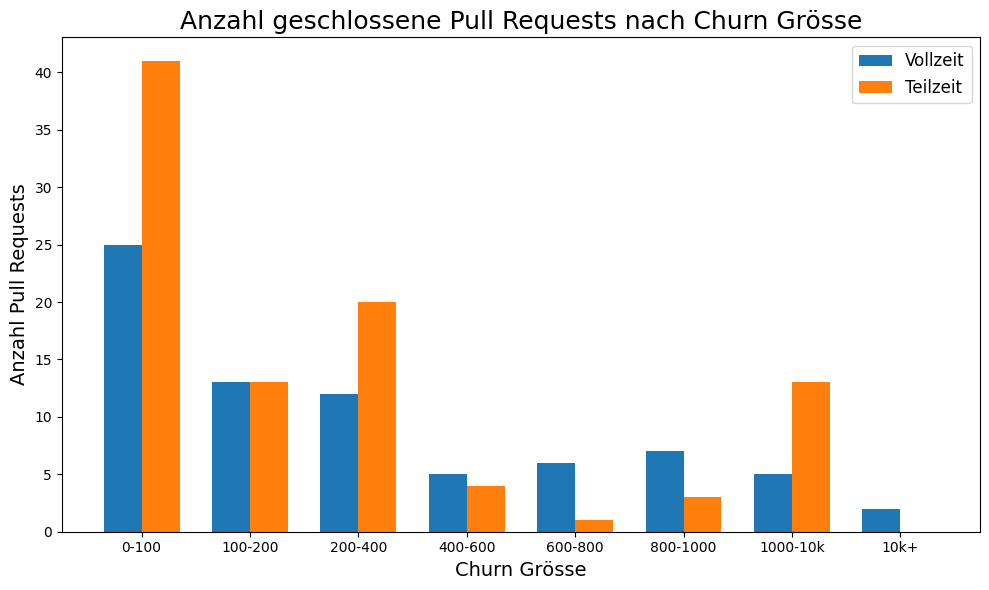
\includegraphics[width=\textwidth]{Figures/anzahl-geschlossene-prs-nach-churn.png}
    \caption{Anzahl geschlossene Pull Requests nach Churn Grösse}
    \label{fig:anz-clsd-prs-nach-churn}
\end{figure}

\pagebreak
\subsection{Ursachenanalyse der geschlossenen PRs}
Für die Ursachenanalyse wurden alle PRs mit einem Churn-Wert grösser als 500 sowie alle mit einem Churn-Wert kleiner als 100 manuell untersucht und den in Kapitel \secref{sec:KategorienGeschlossenePRs} definierten Kategorien zugeordnet. 
Die Verteilung der Ursachen geschlossener PRs ist in Tabelle \autoref{tab:treatments} dargestellt.


\begin{table}[htbp]
\caption{Geschlossene PRs gruppiert nach Ursache}
\label{tab:treatments}
\centering
\begin{tabular}{l l l l l l l}
\toprule
\textbf{Klasse} & 
\makecell{\textbf{OG}} & 
\makecell{\textbf{FPI}} & 
\makecell{\textbf{FNN}} & 
\makecell{\textbf{IA}} & 
\makecell{\textbf{FZB}} & 
\makecell{\textbf{DIV}} \\
\midrule
T < 100& 35 & 1 & 3 & 2 & 0 & 0\\
V < 100& 22 & 1 & 0 & 1 & 1 & 0 \\
T > 500& 22 & 8 & 0 & 2 & 4 & 5 \\
V > 500& 8 & 0 & 1 & 4 & 6 & 0 \\
\bottomrule
\end{tabular}
\end{table}
\newpage
\noindent\textbf{Legende:}
\begin{itemize}
\item[$T$] Alle Teilzeitklassen
\item[$V$] Alle Vollzeitklassen
\item[$< 100$] Churn kleiner 100
\item[$> 500$] Churn grösser 500
\end{itemize}

Die wichtigsten Erkenntnisse aus der Ursachenanalyse sind folgende: Bei kleinen PRs (Churn $<$ 100) dominieren Fälle ohne nachvollziehbaren Schliessungsgrund. Bei grossen PRs (Churn $>$ 500) treten hingegen häufiger strukturierte Gründe auf, etwa ein falscher Zielbranch oder der Ersatz durch einen anderen PR. Teilzeitklassen haben insgesamt mehr PRs ohne klar dokumentierten Grund geschlossen, während Vollzeitklassen etwas häufiger explizite Ablehnungen oder Korrekturen von Branch-Fehlern zeigen.


\subsection{Zeitliche Analyse geschlossener PRs}

Eine Analyse der geschlossenen PRs im zeitlichen Verlauf der Projektlaufzeit zeigt deutliche Unterschiede zwischen Vollzeit- und Teilzeitklassen.

\begin{figure}[htbp] 
\centering \begin{subfigure}[b]{0.48\textwidth} 
\centering 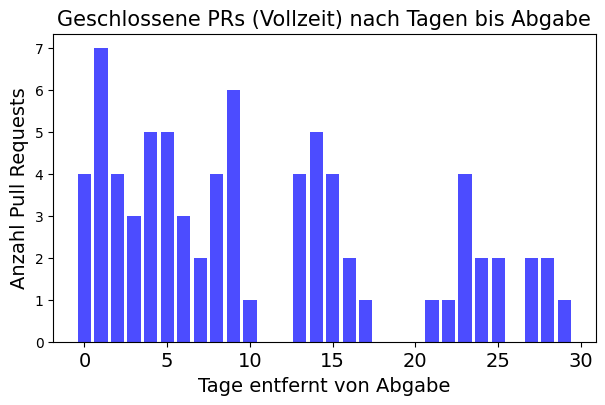
\includegraphics[width=\textwidth]{Figures/closed-prs-projektzeit-vollzeit.png} 
\caption{Geschlossene PRs Vollzeitklassen} 
\label{fig:closed-prs-projektkeit-vollzeit}
\end{subfigure} 
\hfill 
\begin{subfigure}[b]{0.48\textwidth} 
\centering 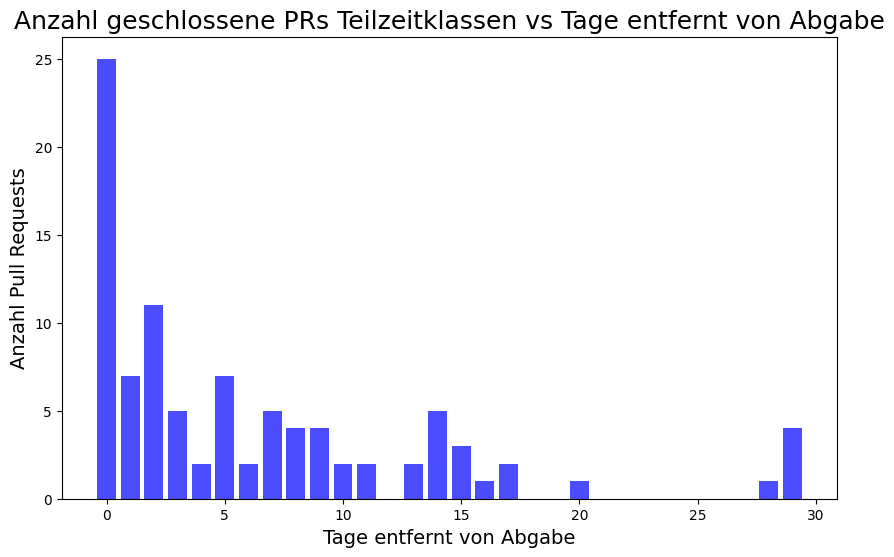
\includegraphics[width=\textwidth]{Figures/closed-prs-projektzeit-teilzeit.png} 
\caption{Geschlossene PRs Teilzeitklassen} 
\label{fig:closed-prs-projektkeit-teilzeit} 
\end{subfigure} 
\caption{Anzahl geschlossener PRs nach Tagen vor Abgabetermin} 
\label{fig:closed-prs-projektzeit} 
\end{figure}

Die wichtigsten Beobachtungen sind folgende: In Teilzeitklassen konzentrieren sich die geschlossenen PRs stark auf die letzten Projekttage, insbesondere auf den Tag der Abgabe. In Vollzeitklassen hingegen verteilen sich die geschlossenen PRs gleichmässiger über den gesamten Projektverlauf.


\subsection{Zusammenfassung}

Zusammenfassend lässt sich festhalten, dass Teilzeitklassen tendenziell mehr kleine PRs ohne ausführliche Begründung schliessen, während Vollzeitklassen grössere PRs strukturierter ablehnen oder gezielt korrigieren. Auffällig ist zudem, dass viele geschlossene PRs, insbesondere in Teilzeitklassen, vermehrt gegen Ende des Projekts auftreten. Darüber hinaus zeigt sich, dass bei PRs mit hohen Churn-Werten Schliessungen häufiger auf Branch-Fehler oder redundante Implementierungen zurückzuführen sind.


\section{Ergebnisse Entwicklungsaktivität}
Empirische Studien zeigen, dass die Entwicklungsaktivität in Open-Source-Projekten auf Plattformen wie GitHub charakteristische Muster im Wochenverlauf aufweist. Insbesondere an Wochenenden ist die Aktivität signifikant geringer als unter der Woche. Innerhalb der Arbeitswoche fallen Montag und Freitag häufig als die Tage mit der geringsten Aktivität auf. Das Phänomen des Rückgangs der Entwicklungsaktivität wird oftmals auch \textit{Friday Effect} genannt. \parencite{claes_programmers_2018}

Dies soll nun im Zusammenhang mit der \fref{forschungsfrage3} "\textit{Lassen sich Patterns der Zusammenarbeit im Team erkennen,
hinsichtlich der Tage, an denen die Studierenden an den Projekten arbeiten?}" anhand der Projektmodule analysiert werden. Um diese Analyse durchführen zu können, werden die Klassen einzeln nach ihren Arbeitstagen analysiert. Die Arbeitstage werden anhand der offenen und geschlossenen Pull Requests und der Commit-Daten definiert. Für dies wird das Mining um die im Kapitel \secref{sec:Metriken} erwähnte Metrik \textit{commit} ergänzt.

Um die Entwicklungsaktivität messbar machen zu können, mussten für alle Klassen die Projektmodul-Unterrichtstage nachgeschlagen werden:
\begin{table}[ht]
\caption{Projektmodul-Unterrichtstage der Klassen}
\label{tab:stundenplan}
\centering
\begin{tabular}{l l l}
\toprule
\textbf{Klasse} & \textbf{Ort} & \textbf{Tag} \\
\midrule
It21tb   & Zürich      & Montag      \\
It21ta   & Zürich      & Montag      \\
It21a    & Zürich      & Mittwoch    \\
It21tb   & Winterthur  & Donnerstag  \\
It21a    & Winterthur  & Freitag     \\
It21b    & Winterthur  & Freitag     \\
It21ta   & Winterthur  & Freitag     \\
\midrule
It23tb   & Zürich      & Montag      \\
It23ta   & Zürich      & Montag      \\
It23a    & Zürich      & Mittwoch    \\
It23b    & Zürich      & Mittwoch    \\
It23a    & Winterthur  & Freitag     \\
It23ta   & Winterthur  & Freitag     \\
It23tb   & Winterthur  & Freitag     \\
\midrule
It24tb   & Zürich      & Montag      \\
It24ta   & Zürich      & Montag      \\
It24a    & Zürich      & Mittwoch    \\
It24a    & Winterthur  & Freitag     \\
It24ta   & Winterthur  & Freitag     \\
It24tb   & Winterthur  & Freitag     \\
\bottomrule
\end{tabular}
\end{table}



Da sich während der Analyse  Differenzen zwischen den Voll- und Teilzeitklassen ergaben, werden diese geteilt angeschaut. 

\subsection{Arbeitstage Pull Requests}
Als erstes werden die Wochentage der Pull Request Erstellungs- und Schliessungsdaten ermittelt und auf die Wochentage aufgeteilt. Diese Aufteilung wird pro Klasse vorgenommen. In den vorliegenden Daten zeigt sich eine Tendenz zur Konzentration der Aktivitäten auf spezifische Wochentage, insbesondere auf die jeweiligen Unterrichtstage. So wurden bei den Vollzeitklassen rund 24\,\% aller Pull Requests (PRs) am Projekttag erstellt. Bei den Teilzeitklassen liegt dieser Wert mit 34\,\% deutlich höher. Dies unterstreicht die Bedeutung des Unterrichtstages für die praktische Arbeit im Rahmen des Projekts.

Die \autoref{fig:anz-prs-teilzeit-pro-wochentag} zeigt exemplarisch die Verteilung der PR-Erstellungen auf die Wochentage für zwei Teilzeitklassen. Deutlich erkennbar ist eine Aktivitätsspitze am jeweiligen Unterrichtstag. An den folgenden Tagen nimmt die Aktivität deutlich ab. Auffällig ist auch, dass am Unterrichtstag nicht nur PRs erstellt, sondern auch überprüft und geschlossen wurden. Insgesamt ist der Anteil der am Wochenende erstellten PRs mit 27.7\,\% vergleichsweise hoch.

\begin{figure}[htbp]
    \centering
    \begin{subfigure}[b]{0.48\textwidth}
        \centering
        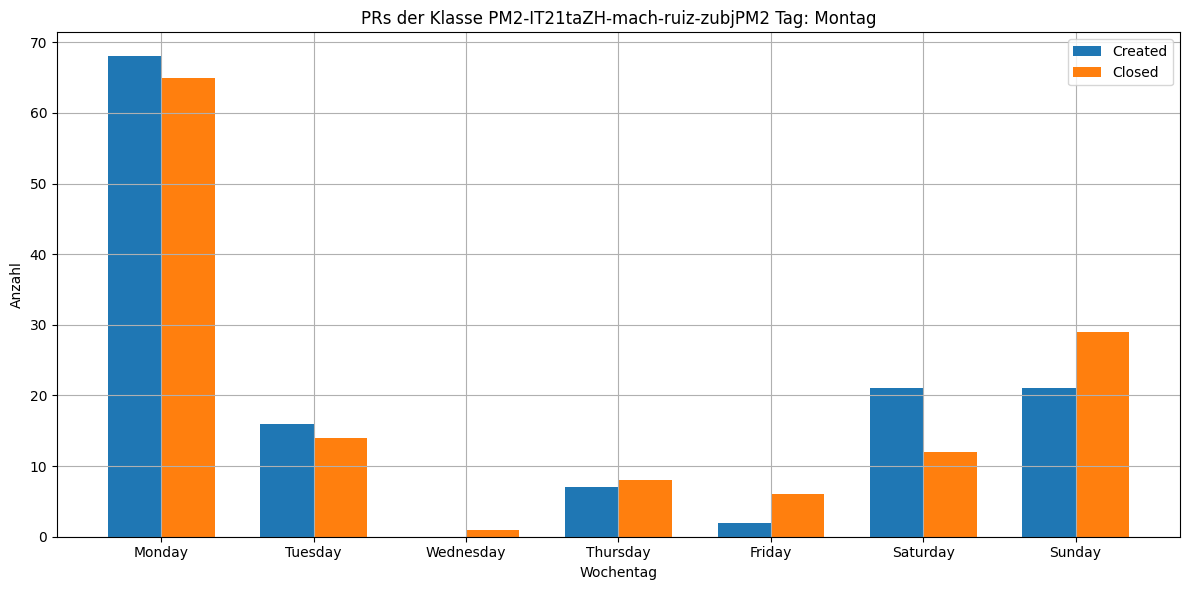
\includegraphics[width=\textwidth]{Figures/pr-klasse-per-wochentag-it21ta.png}
         \caption{Anzahl geöffneter PRs pro Wochentag der Teilzeitklasse It21ta}
        \label{fig:anzahl-prs-pro-wochentag-it21ta}
    \end{subfigure}
    \hfill
    \begin{subfigure}[b]{0.48\textwidth}
        \centering
        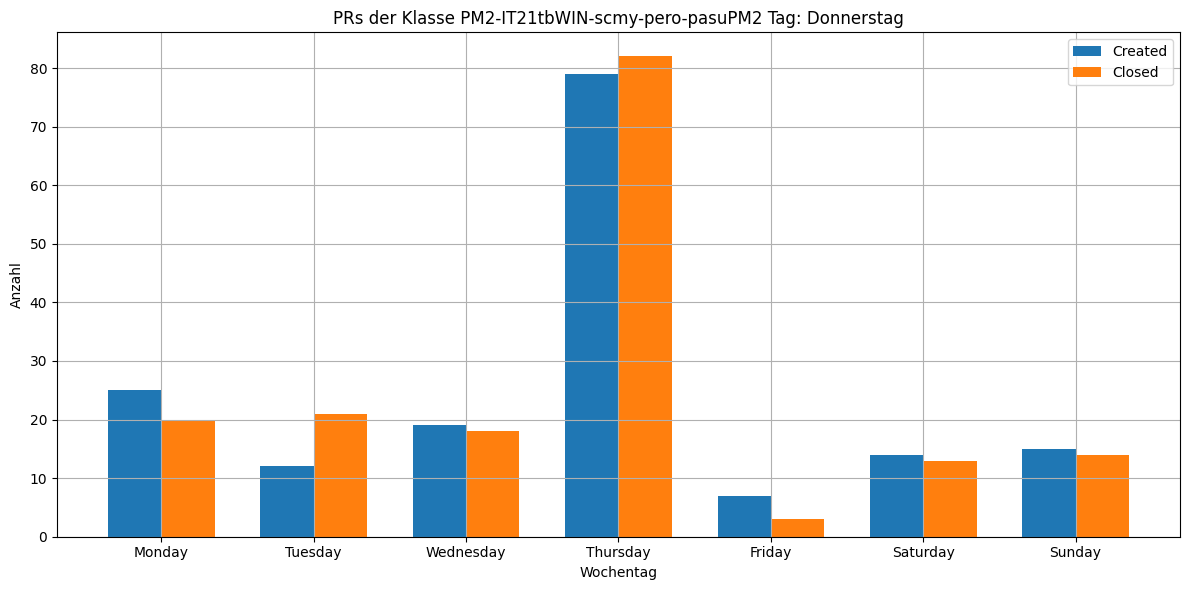
\includegraphics[width=\textwidth]{Figures/pr-klasse-per-wochentag-21tb.png}
         \caption{Anzahl geöffneter PRs pro Wochentag der Teilzeitklasse It21tb}
        \label{fig:anzahl-prs-pro-wochentag-it21tb}
    \end{subfigure}
    \caption{Anzahl geöffneter PRs pro Wochentag von 2 Teilzeitklassen}
    \label{fig:anz-prs-teilzeit-pro-wochentag}
\end{figure}

Ein gegensätzliches Bild zeigt sich bei den Vollzeitklassen. Die \autoref{fig:anz-prs-vollzeit-pro-wochentag} zeigt die Verteilung der PR-Erstellungen und Schliessungen für zwei exemplarische Klassen.
Hier zeigt sich eine insgesamt gleichmässigere Verteilung der Aktivitäten über die Woche. Zwar ist auch hier der Projekttag am aktivsten, jedoch meist in geringerem Ausmass als bei den Teilzeitklassen. Zudem wurden nur 16.8\% der PR am Wochenende erstellt.

\begin{figure}[htbp]
    \centering
    \begin{subfigure}[b]{0.48\textwidth}
        \centering
        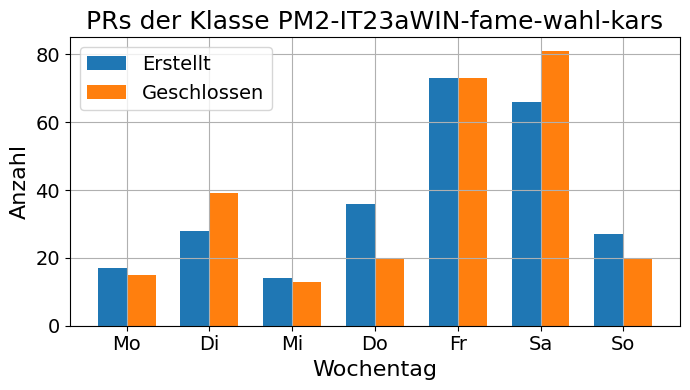
\includegraphics[width=\textwidth]{Figures/pr-klasse-per-wochentag-23a.png}
         \caption{Anzahl geöffneter PRs pro Wochentag der Vollzeitklasse It23a}
        \label{fig:anzahl-prs-pro-wochentag-it23a}
    \end{subfigure}
    \hfill
    \begin{subfigure}[b]{0.48\textwidth}
        \centering
        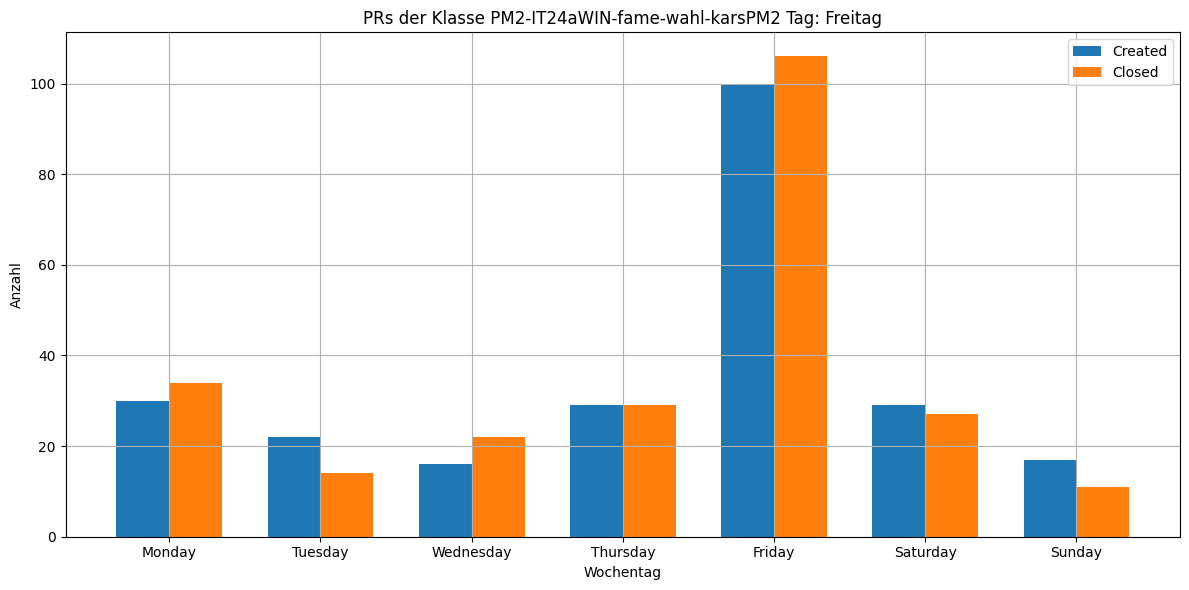
\includegraphics[width=\textwidth]{Figures/pr-klasse-per-wochentag-24a.png}
         \caption{Anzahl geöffneter PRs pro Wochentag der Vollzeitklasse It24a}
        \label{fig:anzahl-prs-pro-wochentag-it24a}
    \end{subfigure}
    \caption{Anzahl geöffneter PRs pro Wochentag von 2 Vollzeitklassen}
    \label{fig:anz-prs-vollzeit-pro-wochentag}
\end{figure}

\subsection{Arbeitstage Commits}
Da sowohl die PRs als auch die einzelnen Commits für die Entwicklungsanalyse von Interesse sind, wurden die Commits der PRs analysiert.
Die Analyse bestätigt die in der PR-Analyse bereits festgestellten Ergebnisse.

So wurden bei den Vollzeitklassen 23.7\,\% aller Commits am jeweiligen Unterrichtstag durchgeführt. Bei den Teilzeitklassen liegt dieser Anteil mit 33.9\,\% deutlich höher. Die \autoref{fig:anz-commits-teilzeit-pro-wochentag} zeigt die Verteilung der Commits über die Wochentage exemplarisch für zwei Teilzeitklassen. Analog zur PR-Verteilung ist eine deutliche Spitze an den jeweiligen Projekttagen erkennbar. Insgesamt wurden 25.9\,\% aller Commits der Teilzeitklassen an einem Samstag oder Sonntag durchgeführt.

\begin{figure}[htbp]
    \centering
    \begin{subfigure}[b]{0.48\textwidth}
        \centering
        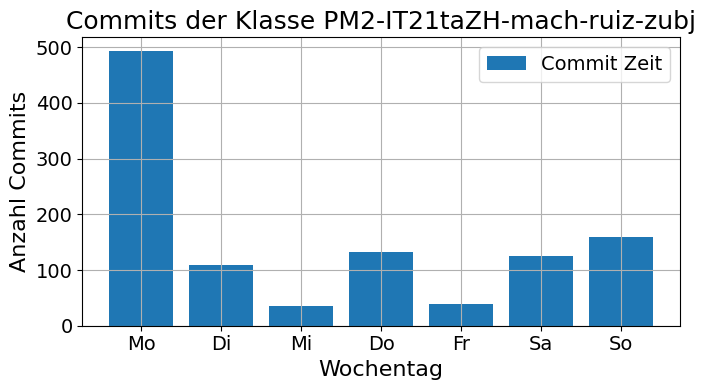
\includegraphics[width=\textwidth]{Figures/commits-klasse-per-wochentag-21ta.png}
         \caption{Anzahl Commits pro Wochentag der Teilzeitklasse It21ta}
        \label{fig:anzahl-commits-pro-wochentag-it21ta}
    \end{subfigure}
    \hfill
    \begin{subfigure}[b]{0.48\textwidth}
        \centering
        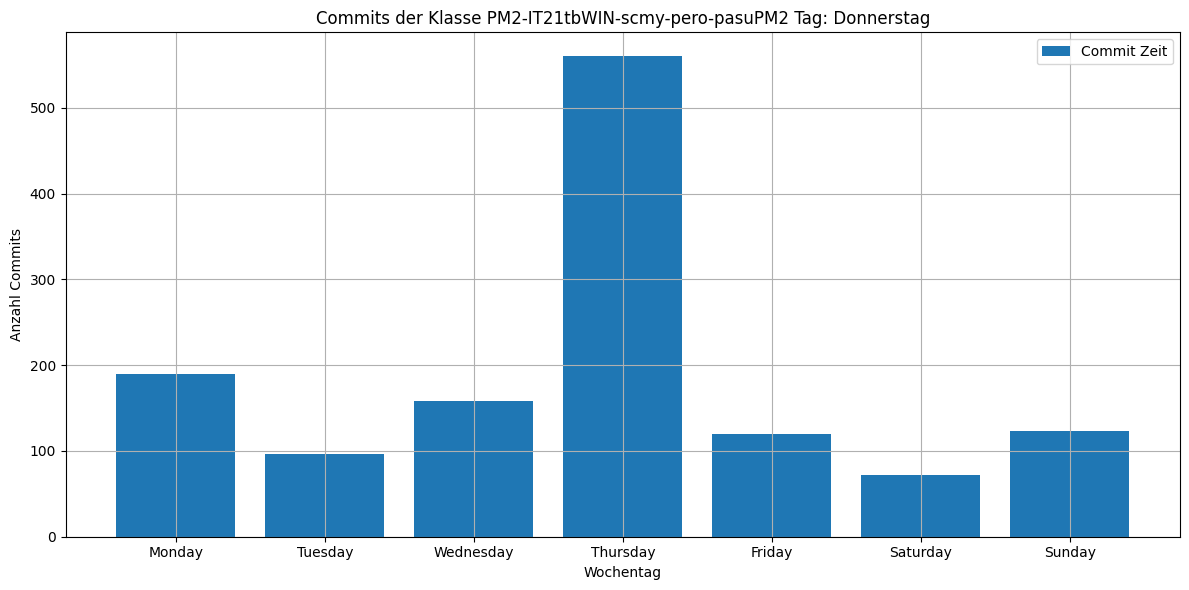
\includegraphics[width=\textwidth]{Figures/commits-klasse-per-wochentag-21tb.png}
         \caption{Anzahl Commits pro Wochentag der Teilzeitklasse It21tb}
        \label{fig:anzahl-commits-pro-wochentag-it21tb}
    \end{subfigure}
    \caption{Anzahl Commits pro Wochentag von 2 Teilzeitklassen}
    \label{fig:anz-commits-teilzeit-pro-wochentag}
\end{figure}

Ein ähnliches Bild ergibt sich auch bei den Vollzeitklassen zwischen Pull Requests und Commits. Die \autoref{fig:anz-commits-vollzeit-pro-wochentag} zeigt die Commits zweier exemplarischer Klassen. Hier wurden 23.7\,\% der Commits am jeweiligen Projekttag durchgeführt – identisch mit dem PR-Anteil. Am Wochenende hingegen wurden nur 19.4\,\% der Commits verzeichnet, was deutlich unter dem Wert der Teilzeitklassen liegt.

\begin{figure}[htbp]
    \centering
    \begin{subfigure}[b]{0.48\textwidth}
        \centering
        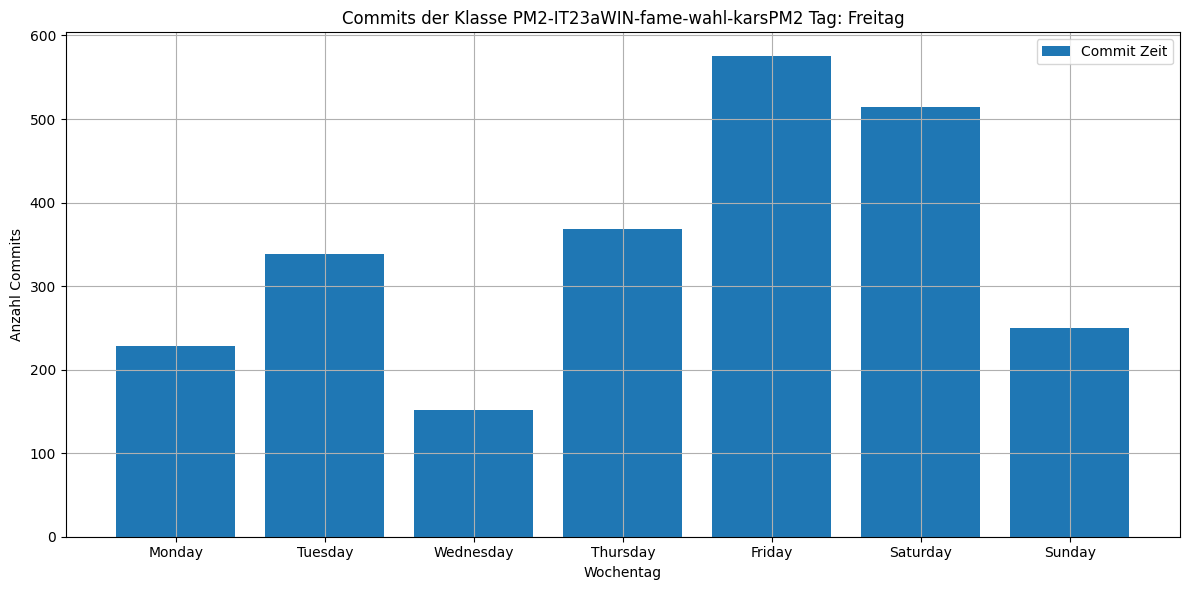
\includegraphics[width=\textwidth]{Figures/commits-klasse-per-wochentag-23a.png}
         \caption{Anzahl Commits pro Wochentag der Teilzeitklasse It23a}
        \label{fig:anzahl-commits-pro-wochentag-it23a}
    \end{subfigure}
    \hfill
    \begin{subfigure}[b]{0.48\textwidth}
        \centering
        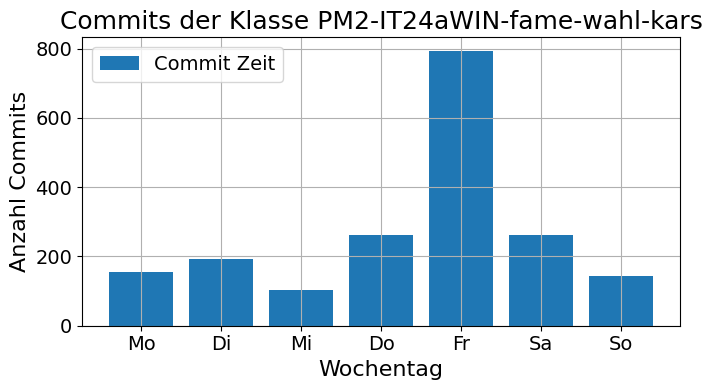
\includegraphics[width=\textwidth]{Figures/commits-klasse-per-wochentag-24a.png}
         \caption{Anzahl Commits pro Wochentag der Teilzeitklasse It24a}
        \label{fig:anzahl-commits-pro-wochentag-it24a}
    \end{subfigure}
    \caption{Anzahl Commits pro Wochentag von 2 Vollzeitklassen}
    \label{fig:anz-commits-vollzeit-pro-wochentag}
\end{figure}

Zusammenfassend lässt sich festhalten, dass es klare Tendenzen gibt, dass die Studierenden vor allem an den Projekttagen arbeiten, wobei die Teilzeitstudierenden noch häufiger am Wochenende arbeiten und die Vollzeitstudierenden die Arbeit eher unter der Woche aufteilen.

\section{Projektmodul Ergebnisse bei Open Source Projekten}
\subsection{Vorstellung der GitHub-Organisationen im Vergleich zu Racetrack-Projekten}
Im Rahmen dieser Analyse werden die Ergebnisse des Racetrack-Projektmoduls mit den Metriken von Open-Source-Projekten verglichen. Hierführ werden drei unterschiedliche Github Organisationen betrachtet, welche eine unterschiedliche Grösse und Komplextität aufweisen: \textit{Ubique}, \textit{Swiss Federal Railways (SBB)} und \textit{
Zalando SE} angeschaut \parencite{noauthor_ubique_nodate} \parencite{noauthor_swiss_nodate} \parencite{noauthor_zalando_nodate}. 


\textit{Ubique Innovation AG} ist ein Schweizer Unternehmen mit Sitz in Zürich, das sich auf die Entwicklung von Softwarelösungen mit Fokus auf Mobile-App-Entwicklung spezialisiert hat. Im Jahr 2021 beschäftigte die Firma rund 50 Mitarbeiter \cite{noauthor_mathias_2021}. Zu den bekanntesten Projekten von Ubique gehören unter anderem die Mobile App der \textbf{Schweizerischen Bundesbahnen (SBB)}, die Kartenapplikation \textbf{Swisstopo} des Bundesamt für Landestopografie sowie die \textbf{Rega App}. \parencite{noauthor_apps_nodate}.

todo: mit 8knot github org aluege (aktuell down) 
https://metrix.chaoss.io/

Die \textit{Schweizerische Bundesbahnen (SBB)} ist die staatliche Eisenbahngesellschaft der Schweiz \parencite{uvek_schweizerische_nodate}. Die SBB repräsentiert eine mittelgrosse Organisation im Bereich der Open Source Entwicklung mit 104 Projekten und 137 Followers auf Github. \parencite{noauthor_swiss_nodate} 
todo: same 8knot analyse

Zalando ist eine grosse Github Organisation, die für ihre umfangreichen Open-Source-Projekte im Bereich der E-Commerce- und Cloud-Computing-Technologien bekannt ist. So besitzt Zalando 50 Repositories mit 835 Follower. \parencite{noauthor_zalando_nodate}

\subsection{Latency und Churn}
\subsection{Allgemeine Korrelationen}

 
%% Indicate the main file. Must go at the beginning of the file.
% !TEX root = ../main.tex

%----------------------------------------------------------------------------------------
% CHAPTER TEMPLATE
%----------------------------------------------------------------------------------------


\chapter{Diskussion und Ausblick} % Main chapter title

\label{Chapter5} % Change X to a consecutive number; for referencing this chapter elsewhere, use \ref{ChapterX}

%----------------------------------------------------------------------------------------
% SECTION 1
%----------------------------------------------------------------------------------------

\section{Diskussion}

Wie in der Aufgabenstellung beschrieben, wurden im Rahmen einer Literaturrecherche relevante Metriken identifiziert und aus den Repositories extrahiert. Auf dieser Grundlage wurden sechs Forschungsfragen definiert, die sich auf spezifische Metriken beziehen und deren Zusammenhänge untersuchen sollen. In diesem Kapitel werden die Forschungsfragen erneut aufgegriffen, eingeordnet und im Kontext der gewonnenen Erkenntnisse diskutiert.


\subsection{Diskussion Forschungsfrage 1: Zusammenhang Latency und Churn}
Wie im Abschnitt \secref{sec:PullRequestDauer} erwähnt, besteht in der Fachliteratur keine Einigkeit über den Zusammenhang zwischen den beiden Metriken \textit{Churn} und \textit{Latency} \parencite{yu_wait_2015}\parencite{hasan_understanding_2023}\parencite{kudrjavets_small_2022}. \\
Die Ergebnisse (\secref{sec:ResultatChurnLatency}) dieser Forschungsfrage zeigen keinen Zusammenhang, weder mit noch ohne Ausreisser. Der Spearman-Koeffizient fällt hierfür zu gering aus. \\
Berücksichtigt man zusätzlich den Kontext aus \fref{forschungsfrage3}, wird deutlich, dass die Projektdauer Einfluss auf die \textit{Latency} hat. Gegen Ende eines Projekts verkürzt sich die \textit{Latency}, während der \textit{Churn} zunimmt. Dieser gegenläufige Verlauf schwächt einen direkten Zusammenhang zwischen \textit{Churn} und \textit{Latency} ab. \\
Die Korrelationsanalyse der Racetrack-Repositories zeigt zudem, dass andere Metriken, wie etwa die Anzahl der Kommentare, Einfluss auf die \textit{Latency} haben, jedoch nicht auf den \textit{Churn}. Da Kommentare auf Änderungsbedarf hinweisen können, und dies unabhängig von der \textit{Churn}-Metrik, erklärt  ebenfalls, warum zwischen \textit{Latency} und \textit{Churn} kein klarer Zusammenhang besteht. \\
Zusätzlich besteht auch kein Zusammenhang zwischen \textit{Latency} und \textit{Churn} in den Korrelationsanalysen von den überprüften OSS-Projekten in Kapitel \secref{sec:Korrelationsanalyse}. Dies zeigt, dass die nicht zusammenhängenden Metriken kein ausschliessliches Phänomen von den Racetrack-Repositories sind.

Anhand unserer Ergebnisse wird deutlich, dass Pull-Requests ein komplexes Konstrukt sind und sich die \textit{Latencies} der Pull-Requests aus vielen verschiedenen Gegebenheiten und somit Metriken zusammensetzen.

\subsection{Diskussion Forschungsfrage 2: Schliessgründe der PRs}
Die Untersuchung der Schliessgründe von Pull-Requests (\secref{sec:UntersuchungSchliessgründePRs}) zeigt, dass besonders häufig die Kategorie \textit{OG} (ohne erkennbaren Grund) auftritt, vor allem bei kleineren PRs mit einem Churn unter 100. Dies deutet darauf hin, dass kleinere Änderungen tendenziell weniger dokumentiert und begründet geschlossen werden. \\
Bei den  Teilzeitklassen tritt dieses Verhalten deutlich häufiger auf. Eine mögliche Erklärung dafür ist Zeitmangel oder eine geringere Relevanz kleinerer Änderungen im Vergleich zu grösseren / wichtigeren Beiträgen. Ebenfalls zeigen die Analysen in \secref{sec:ErgebnisseEntwicklungsaktivtät}, dass die Pull-Requests oftmals an den Projektmodul-Unterrichtstagen geschlossen werden. Deshalb könnte es sein, dass die Reviews in Person und daher ohne Dokumentation durchgeführt werden. 

Bei PRs mit einem grossem Churn zeigen sich in den Vollzeitklassen häufiger strukturierte Schliessgründe wie \textit{ZFB} (falscher Zielbranch) oder \textit{IA} (Implementierung
abgelehnt). Bei den Teilzeitklassen sind es \textit{FPI} (Feature durch anderen
PR implementiert) und \textit{DIV} (Divers). Bei beiden ist jedoch die Kategorie \textit{OG} (ohne erkennbaren Grund) am häufigsten vertreten. \\
Die hohe Anzahl an PRs ohne erkennbaren Grund legt nahe, dass die Kommunikation über andere Kanäle (z.B. Microsoft Teams, Jira, WhatsApp) oder direkt vor Ort erfolgt. In solchen Fällen werden Pull-Requests möglicherweise mündlich besprochen und im Anschluss geschlossen, ohne dass ein schriftlicher Kommentar im PR selbst hinterlassen wird.

Die normalisierten Daten zeigen, dass in Vollzeitklassen durchschnittlich mehr PRs pro Projekt geschlossen werden. Dies kann darauf hindeuten, dass der Review-Prozess dort konsequenter durchgeführt wird.

Ein weiterer Unterschied zeigt sich im zeitlichen Verlauf der Schliessungen. In Teilzeitklassen treten viele geschlossene PRs erst in den letzten Tagen des Projekts auf, besonders am Tag der Abgabe. In den Vollzeitklassen sind die Schliessungen gleichmässiger über den gesamten Projektverlauf verteilt.  \\
Diese Häufung zum Projektende in Teilzeitklassen könnte mehrere Ursachen besitzen: Zum einen stehen Teilzeitstudierenden durch ihre beruflichen Verpflichtungen während des Semesters oftmals nur ein begrenztes Zeitfenster für die Projektarbeit zur Verfügung. Meistens bündelt sich dies auf die Unterrichtstage oder Abende. Des Weiteren ist die synchrone Abstimmung innerhalb der Teams durch die eingeschränkte Verfügbarkeit der Mitglieder erschwert, was zu einer Ansammlung offener PRs führen kann. Ebenfalls scheint der Fokus in Teilzeitklassen eher auf der termingerechten Abgabe als auf einem optimierten Entwicklungsprozess zu liegen, was zur Folge hat, dass viele PRs erst kurz vor Projektende finalisiert werden.

Zusammenfassend lässt sich feststellen, dass sich die Schliessgründe von Pull-Requests nicht zuverlässig klassifizieren lassen. Viele Pull-Requests werden ohne erkennbaren Grund geschlossen. Bei den klassifizierbaren PRs zeigen sich Unterschiede sowohl in der Verteilung der Gründe als auch in der zeitlichen Struktur. Vollzeitklassen schliessen PRs tendenziell strukturierter und über den gesamten Projektverlauf verteilt, während Teilzeitklassen häufiger spontane oder unkommentierte Schliessungen am Projektende aufweisen.


\subsection{Diskussion Forschungsfrage 3: Zusammenhang Projektverlauf auf Review-Dauer}
Die Ergebnisse der \fref{forschungsfrage3} zeigen deutlich, dass die \textit{latency} im Verlauf der Projekte abnimmt, obwohl gleichzeitig die \textit{Churn}-Werte steigen. Besonders an den letzten Tagen vor Projektende wurden viele Pull-Requests sehr schnell geschlossen, teilweise in einer Geschwindigkeit, die keine regulären und genauen Reviews mehr zulässt. 

Dabei ist zu beachten, dass diese Projekte, wie bereits in Kapitel \secref{sec:Projektmodule} erwähnt, einen festen Abgabetermin haben und eine verspätete Abgabe Auswirkungen auf die Bewertung hat. Eine naheliegende Erklärung ist, dass Studierende in den letzten Tagen vor Abgabe versuchen, möglichst viele Funktionalitäten zu implementieren und bestehende Fehler zu beheben. Daraus ergibt sich eine grosse Anzahl an Pull-Requests, die unter Zeitdruck schnell gemergt werden. \\
Dieser Zeitdruck kann zur Folge haben, dass Reviews nur oberflächlich oder gar nicht durchgeführt werden. In manchen Fällen erfolgt die Entwicklung möglicherweise im Pair-Programming (zwei Entwickler programmieren zusammen auf einem Notebook), wodurch ein separates Review entfällt, da der Code gemeinsam erstellt wurde.

\subsection{Diskussion Forschungsfrage 4: Patterns der Zusammenarbeit hinsichtlich der Arbeitstage}
Die Analyse der Arbeitstage von Pull-Requests (\secref{sec:ErgebnisseEntwicklungsaktivtät}) zeigt deutliche Unterschiede der Arbeitstage zwischen Vollzeit- und Teilzeitklassen. Bei der Betrachtung der Tage, an denen PRs erstellt und bearbeitet wurden, fällt auf, dass sich die Aktivitäten in den Teilzeitklassen stark auf spezifische Wochentage konzentrieren, insbesondere auf die Unterrichtstage. 

Die Auswertung der Erstellungsdaten zeigt, dass in Teilzeitklassen ein Grossteil der PRs an den Unterrichtstagen sowie an Wochenenden erstellt wird. Eine mögliche Erklärung ist, dass Teilzeitstudierende unter der Woche aufgrund anderer Verpflichtungen im privaten oder beruflichen Umfeld nur eingeschränkt Zeit für Projektarbeit finden.

Bei den Vollzeitklassen zeigt sich hingegen eine gleichmässigere Verteilung der Pull-Request-Aktivitäten über die Woche. Diese Gruppen arbeiten typischerweise an allen Wochentagen ausser am Wochenende, was auf eine kontinuierlichere Arbeitsweise hinweist. Der Mittwoch respektive der entsprechende Unterrichtstag der Klasse sticht hier besonders heraus, da an diesem Tag vergleichsweise viele PRs erstellt und bearbeitet wurden. Eine mögliche Erklärung dafür könnte sein, dass an diesem Tag oftmals Gruppensitzungen oder gemeinsame Entwicklungstreffen (\textit{Weeklys}) stattfinden. \\
Diese unterschiedlichen Arbeitsrhythmen der beiden Unterrichtsmodelle bedeuten, dass Dozierende auf verschiedene Rahmenbedingungen treffen. Diese sollten bei Betreuung und Bewertung der Projekte berücksichtigt werden.

\subsection{Diskussion Forschungsfrage 5: Unterschiede Voll- und Teilzeitklassen hinsichtlich Nutzung der PRs}
In der \fref{forschungsfrage5} wurde untersucht, ob Unterschiede in der Nutzung von Pull-Requests zwischen den Vollzeit- und Teilzeitklassen bestehen, insbesondere im Hinblick auf Anzahl, Umfang (Churn) und Bearbeitungsdauer (Latency).

Im Median zeigen die Unterschiede bei den Churns keine signifikanten Unterschiede auf. Betrachtet man jedoch den Mittelwert, so liegt dieser bei den Vollzeitstudierenden um rund 40 Zeilen höher. Zudem ist die Standardabweichung bei den Vollzeitklassen deutlich grösser (+286), was auf eine grössere Streuung der Änderungsumfänge hindeutet. Auch der maximale Churn-Wert ist in dieser Gruppe deutlich höher. \\
Eine detaillierte Analyse zeigt, dass beide Unterrichtsmodelle den grössten Anteil ihrer Pull-Requests mit Änderungen im Bereich von 50–199 Zeilen einreichen. Sehr grosse Pull-Requests (über 10.000 Zeilen) sind in beiden Gruppen selten, treten jedoch bei den Vollzeitstudierenden etwas häufiger auf. Dies erklärt die grössere Streuung. Bemerkenswert ist jedoch, dass 40\,\% dieser sehr grossen PRs von den Vollzeitstudierenden wieder geschlossen wurden, was darauf hindeutet, dass solche umfangreichen Änderungen nicht automatisch akzeptiert werden.


Hinsichtlich der Latency ergibt sich ein unterschiedliches Bild: Der Median ist bei den Teilzeitstudierenden geringer, was auf eine insgesamt schnellere durchschnittliche Bearbeitung hindeutet. Gleichzeitig sind jedoch sowohl der Mittelwert als auch die Standardabweichung höher, verursacht durch einige sehr lange Pull-Requests. Die Extremwerte zeigen, dass Teilzeitstudierende sowohl sehr kurze PRs (unter einer Minute) als auch sehr lange (über sieben Tage) häufiger haben als ihre Vollzeitpendants.

Die meisten Pull-Requests in beiden Gruppen werden innerhalb von 30 Minuten bearbeitet. Die längeren Bearbeitungszeiten bei den Teilzeitstudierenden lassen sich plausibel durch das in \fref{forschungsfrage4} aufgezeigte Arbeitsverhalten erklären: Da die Projektarbeit hauptsächlich an bestimmten Unterrichtstagen erfolgt, bleiben PRs unter der Woche häufiger liegen.

Im Durchschnitt erstellen Vollzeitstudierende acht Pull-Requests mehr pro Projekt als die Teilzeitstudierenden. Ein klarer Grund für diesen Unterschied lässt sich aus den übrigen Daten nicht ableiten, insbesondere da weder kleinere Churns noch kürzere Latencies bei den Vollzeitgruppen dominieren. 

\subsection{Diskussion Forschungsfrage 6: Unterschiede der Repository-Metriken zwischen Studentenprojekten und professionellen GitHub-Organisationen}
Die für die \fref{forschungsfrage6} benötigte Analyse der Repository-Metriken zwischen den Studentenprojekten (Racetrack-Repositories) und den professionellen GitHub-Organisationen Ubique, Schweizerische Bundesbahn (SBB) und Zalando zeigt spezifische Unterschiede, welche anhand mehrerer Korrelations-Heatmaps visualisiert wurden. 

Im Vergleich mit Ubique zeigen die Racetrack-Repositories stärkere positive Korrelationen zwischen \textit{Description Length} und \textit{Commits} sowie \textit{Description Length} und \textit{Churn}. Dies deutet darauf hin, dass in den Studentenprojekten lange Beschreibungen häufiger mit grossen Änderungen und mehreren Commits verbunden sind. Dies kann als Hinweis dienen, dass bei den Projektmodul-Repositories verstärkt auf das Erklären der Änderungen und auf das Reflektieren im Review-Prozess geachtet wird, möglicherweise als Teil der Bewertungskriterien. 

Der Vergleich mit der Schweizerischen Bundesbahnen (SBB) zeigt, dass die Race\-track-Projekte eine stärkere positive Korrelation zwischen \textit{Description Length} und \textit{Commits} sowie \textit{Churn} haben. Zudem besitzen die Racetrack-Projekte eine etwas schwächere Korrelation zwischen \textit{Comments} und den anderen Metriken im Vergleich zur SBB.

Im Gegensatz dazu zeigt sich bei Zalando eine negative Korrelation zwischen \textit{Description Length} und \textit{Churn}, was bedeutet, dass grössere Änderungen tendenziell weniger ausführlich dokumentiert werden. Dies könnte auf optimierte, informellere oder stärker automatisierte Prozesse in professionellen Organisationen hindeuten. Ebenfalls muss berücksichtigt werden, dass bei grösseren OpenSource-Projekten, über welche Zalando mehrere verfügt (z.B. Postgres Kubernetes Operator, Skipper HTTP Router oder Logbook), diverse PRs aus der Community stammen und dementsprechend weniger standardisiert oder formal beschrieben sind \parencite{noauthor_zalandologbook_2025} \parencite{noauthor_zalandoskipper_2025} \parencite{noauthor_zalandopostgres-operator_2025}.

Zusammenfassend lassen sich die wesentlichen Unterschiede zwischen den untersuchten Studentenprojekten und professionellen Organisationen vor allem in der Art und Weise der Beschreibung und Dokumentation von Pull-Requests zeigen. Die Racetrack-Projekte verwenden tendenziell längere und detailliertere Beschreibungen bei grösseren Änderungen, während in den untersuchten professionellen Organisationen diese Zusammenhänge weniger deutlich oder sogar negativ ausgeprägt sind.


\pagebreak
\section{Ausblick}
Die vorliegenden Analysen liefern diverse Einblicke in das Pull-Request-Verhalten der Studierenden, insbesondere in den Projektmodul-Repositories. 
Auf Basis der gewonnenen Erkenntnisse ergeben sich verschiedene Punkte zur weiterführenden Forschung sowie der konkreten Erweiterung des \textit{GitGauge}-Tools. 

\subsection{Erweiterung von GitGauge}
Die im Rahmen dieser Arbeit untersuchten Metriken könnten teilweise direkt in GitGauge-Auswertungen aufgenommen werden. Besonders interessant wären:
\begin{itemize}
\item \textbf{Automatisierte Klassifikation von Schliessgründen}: Die Kategorisierung der Pull-Request Schliessgründe erfolgte in dieser Arbeit manuell. Eine automatisierte Erkennung auf Basis der Kommentaranalyse mittels eines \textit{LLMs} könnte implementiert werden. Dies könnte dazu führen, dass die Gründe besser klassifiziert werden können. Dadurch stünde Dozierenden eine zusätzliche Metrik zur Beurteilung der Teamkommunikation und des Review-Prozesses zur Verfügung.
\item \textbf{Integration von CI/CD-Metriken}: Derzeit werden CI/CD (\textit{Continuous Integration- und Deployment}) Metriken in GitGauge nicht berücksichtigt, da CI/CD in den Projektmodulen PM1, PM2 und PM3 nicht Teil des Lehrplans ist. Für eine erweiterte Nutzung des Tools, insbesondere für das Projektmodul 4 oder im professionellen Umfeld, wäre die Integration von Metriken wie Build-Zeit, Testdurchläufe oder Anzahl fehlgeschlagener Pipelines eine wertvolle Erweiterung.
\item \textbf{Analyse von Teamdynamiken}: Ergänzend zu den bestehenden Metriken könnten neue Visualisierungen zur Zusammenarbeit innerhalb der Teams implementiert werden. Beispielsweise könnten Netzwerkdiagramme auf Basis von Kommentaren aufzeigen, welche Teammitglieder miteinander interagieren. Ein Aktivitätsindex pro Person würde darüber hinaus helfen, individuelle Beiträge transparenter darzustellen. Solche Visualisierungen könnten zudem verdeutlichen, ob es innerhalb eines Teams isolierte Untergruppen (\textit{Inseln}) gibt oder ob eine gleichmässige Zusammenarbeit stattfindet.
\end{itemize}

\subsection{Weiterführende Forschung}
Aus den in dieser Arbeit durchgeführten Analysen ergeben sich weiterführende Fragestellungen, die über die aktuellen Projektmodule hinausgehen:
\begin{itemize}
\item \textbf{Nachhaltigkeit und weitere Metriken durch CI/CD}: Insbesondere für das Projektmodul PM4 oder externe Industrieprojekte könnte untersucht werden, wie sich \textit{CI/CD} auf Qualität und Reviewprozesse auswirkt. So könnte ein Fokus auf nachhaltige Praktiken gelegt werden. Beispielsweise indem Tests selektiv ausgeführt werden (z.B. nur beim Öffnen eines Pull-Requests anstatt bei jedem Commit), um Ressourcen zu schonen und die Effizienz zu steigern.
\item \textbf{Vergleich mit Enterprise-Projekten}: Eine Erweiterung des Vergleichs zwischen den Studierendenprojekten und professionellen Organisationen könnte weitere Unterschiede in Kultur, Formalisierung und Tooling aufdecken. Besonders spannend wären Analysen von grossen Organisationen, welche keine öffentliche GitHub Organisation besitzen.
\item \textbf{Einfluss von Teamstruktur und Berufserfahrung}: Die aktuell untersuchten Unterschiede zwischen Vollzeit- und Teilzeitstudierenden könnten noch detaillierter hinsichtlich Berufserfahrung, Vorwissen oder Teamkonstellation analysiert werden.
\end{itemize}


\subsection{Fazit}

Die Ergebnisse dieser Arbeit zeigen, dass Pull-Requests mehr als nur ein technisches Tool im Entwicklungsprozess sind. Sie spiegeln auch die Dynamik von Teamprozessen, Zeitmanagement und Kommunikationsverhalten wider. Durch gezieltes Repository-Mining lassen sich daraus wertvolle Erkenntnisse für die Lehre, Projektsteuerung und Prozessverbesserung gewinnen.

Die analysierten Metriken liefern dabei konkrete Ansatzpunkte, um Qualität, Zusammenarbeit und Nachhaltigkeit zu messen.
Die vorliegenden Resultate bilden eine solide Basis für weiterführende Forschungsarbeiten, etwa zur Wirkung von CI/CD-Praktiken, zur Analyse von Teamstrukturen oder zum Vergleich mit industriellen Projekten. 
%% Indicate the main file. Must go at the beginning of the file.
% !TEX root = ../main.tex

%----------------------------------------------------------------------------------------
% CHAPTER 1
%----------------------------------------------------------------------------------------



\chapter{Introduction to \LaTeX} % Main chapter title
\label{Chapter6} % For referencing the chapter elsewhere, use \ref{Chapter1} 

%----------------------------------------------------------------------------------------

% Define some commands to keep the formatting separated from the content
% Placing such commands in the preamble is a good idea.
\newcommand{\keyword}[1]{\textbf{#1}}
\newcommand{\tabhead}[1]{\textbf{#1}}
\newcommand{\code}[1]{\texttt{#1}}
\newcommand{\file}[1]{\texttt{\bfseries#1}}
\newcommand{\option}[1]{\texttt{\itshape#1}}

%----------------------------------------------------------------------------------------

\section{Welcome and Thank You}
 Hello Welcome to this \LaTeX{} Thesis Template, a beautiful and easy to use template for writing a thesis using the \LaTeX{} typesetting system.

If you are writing a thesis (or will be in the future) and its subject is technical or mathematical (though it doesn't have to be), then creating it in \LaTeX{} is highly recommended as a way to make sure you can just get down to the essential writing without having to worry over formatting or wasting time arguing with your word processor.

\LaTeX{} is easily able to professionally typeset documents that run to hundreds or thousands of pages long. With simple mark-up commands, it automatically sets out the table of contents, margins, page headers and footers and keeps the formatting consistent and beautiful. One of its main strengths is the way it can easily typeset mathematics, even \emph{heavy} mathematics. Even if those equations are the most horribly twisted and most difficult mathematical problems that can only be solved on a super-computer, you can at least count on \LaTeX{} to make them look stunning.

%----------------------------------------------------------------------------------------

\section{Learning \LaTeX{}}

\LaTeX{} is not a \textsc{wysiwyg} (What You See is What You Get) program, unlike word processors such as Microsoft Word or Apple's Pages. Instead, a document written for \LaTeX{} is actually a simple, plain text file that contains \emph{no formatting}. You tell \LaTeX{} how you want the formatting in the finished document by writing in simple commands amongst the text, for example, if I want to use \emph{italic text for emphasis}, I write the \verb|\emph{text}| command and put the text I want in italics in between the curly braces. This means that \LaTeX{} is a \enquote{mark-up} language, very much like HTML.

\subsection{A (not so short) Introduction to \LaTeX{}}

If you are new to \LaTeX{}, there is a very good eBook -- freely available online as a PDF file -- called, \enquote{The Not So Short Introduction to \LaTeX{}}. The book's title is typically shortened to just \emph{lshort}. You can download the latest version (as it is occasionally updated) from here:
\url{http://www.ctan.org/tex-archive/info/lshort/english/lshort.pdf}

It is also available in several other languages. Find yours from the list on this page: \url{http://www.ctan.org/tex-archive/info/lshort/}

It is recommended to take a little time out to learn how to use \LaTeX{} by creating several, small `test' documents, or having a close look at several templates on:\\ 
\url{http://www.LaTeXTemplates.com}\\ 
Making the effort now means you're not stuck learning the system when what you \emph{really} need to be doing is writing your thesis.

\subsection{A Short Math Guide for \LaTeX{}}

If you are writing a technical or mathematical thesis, then you may want to read the document by the AMS (American Mathematical Society) called, \enquote{A Short Math Guide for \LaTeX{}}. It can be found online:

\url{http://www.ams.org/tex/amslatex.html} $\rightarrow$ \enquote{Additional Documentation}\\
\url{https://mirror.foobar.to/CTAN/info/short-math-guide/}

\subsection{Common \LaTeX{} Math Symbols}
There are a multitude of mathematical symbols available for \LaTeX{} and it would take a great effort to learn the commands for them all. The most common ones you are likely to use are shown on this page:
\url{http://www.sunilpatel.co.uk/latex-type/latex-math-symbols/}

You can use this page as a reference or crib sheet, the symbols are rendered as large, high quality images so you can quickly find the \LaTeX{} command for the symbol you need.

\subsection{\LaTeX{} on a Mac}
 
The \LaTeX{} distribution is available for many systems including Windows, Linux and Mac OS X. The package for OS X is called MacTeX and it contains all the applications you need -- bundled together and pre-customized -- for a fully working \LaTeX{} environment and work flow.
 
MacTeX includes a custom dedicated \LaTeX{} editor called TeXShop for writing your `\file{.tex}' files and BibDesk: a program to manage your references and create your bibliography section just as easily as managing songs and creating playlists in iTunes.

%----------------------------------------------------------------------------------------

\section{Getting Started with this Template}

If you are familiar with \LaTeX{}, then you should explore the directory structure of the template and then proceed to place your own information into the \emph{THESIS INFORMATION} block of the \file{main.tex} file. You can then modify the rest of this file to your unique specifications based on your degree/university. Section \ref{FillingFile} on page \pageref{FillingFile} will help you do this. Make sure you also read section \ref{ThesisConventions} about thesis conventions to get the most out of this template.

If you are new to \LaTeX{} it is recommended that you carry on reading through the rest of the information in this document.

Before you begin using this template you should ensure that its style complies with the thesis style guidelines imposed by your institution. In most cases this template style and layout will be suitable. If it is not, it may only require a small change to bring the template in line with your institution's recommendations. These modifications will need to be done on the \file{MastersDoctoralThesis.cls} file.

\subsection{About this Template}

This \LaTeX{} Thesis Template is originally based and created around a \LaTeX{} style file created by Steve R.\ Gunn from the University of Southampton (UK), department of Electronics and Computer Science. You can find his original thesis style file at his site, here:
\url{http://www.ecs.soton.ac.uk/~srg/softwaretools/document/templates/}

Steve's \file{ecsthesis.cls} was then taken by Sunil Patel who modified it by creating a skeleton framework and folder structure to place the thesis files in. The resulting template can be found on Sunil's site here:
\url{http://www.sunilpatel.co.uk/thesis-template}


Sunil's template was made available through \url{http://www.LaTeXTemplates.com}, where it was modified many times based on user requests and questions. Version 2.0 and onwards of this template represents a major modification to Sunil's template and is, in fact, hardly recognisable. The work to make version 2.0 possible was carried out by \href{mailto:vel@latextemplates.com}{Vel} and Johannes Böttcher.

Based on Sunil's Version 2.0, Matteo updated the template and incorporated ZHAW University thesis guidelines.

%----------------------------------------------------------------------------------------

\section{What this Template Includes}

\subsection{Folders}

This template comes as a single zip file that expands out to several files and folders. The folder names are mostly self-explanatory:

\keyword{Appendices} -- this is the folder where you put the appendices. Each appendix should go into its own separate \file{.tex} file. An example and template are included in the directory.

\keyword{Chapters} -- this is the folder where you put the thesis chapters. A thesis usually has about six chapters, though there is no hard rule on this. Each chapter should go in its own separate \file{.tex} file and they can be split as:
\begin{itemize}
\item Chapter 1: Introduction to the thesis topic
\item Chapter 2: Background information and theory
\item Chapter 3: (Laboratory) experimental setup
\item Chapter 4: Details of experiment 1
\item Chapter 5: Details of experiment 2
\item Chapter 6: Discussion of the experimental results
\item Chapter 7: Conclusion and future directions
\end{itemize}
This chapter layout is specialised for the experimental sciences, your discipline may be different.

\keyword{Figures} -- this folder contains all figures for the thesis. These are the final images that will go into the thesis document.

\subsection{Files}

Included are also several files, most of them are plain text and you can see their contents in a text editor. After initial compilation, you will see that more auxiliary files are created by \LaTeX{} or BibTeX and which you don't need to delete or worry about:

\keyword{example.bib} -- this is an important file that contains all the bibliographic information and references that you will be citing in the thesis for use with BibTeX. You can write it manually, but there are reference manager programs available that will create and manage it for you. Bibliographies in \LaTeX{} are a large subject and you may need to read about BibTeX before starting with this. Many modern reference managers will allow you to export your references in BibTeX format which greatly eases the amount of work you have to do.

\keyword{MastersDoctoralThesis.cls} -- this is an important file. It is the class file that tells \LaTeX{} how to format the thesis. 

\keyword{main.pdf} -- this is your beautifully typeset thesis (in the PDF file format) created by \LaTeX{}. It is supplied in the PDF with the template and after you compile the template you should get an identical version.

\keyword{main.tex} -- this is an important file. This is the file that you tell \LaTeX{} to compile to produce your thesis as a PDF file. It contains the framework and constructs that tell \LaTeX{} how to layout the thesis. It is heavily commented so you can read exactly what each line of code does and why it is there. After you put your own information into the \emph{THESIS INFORMATION} block -- you have now started your thesis!

Files that are \emph{not} included, but are created by \LaTeX{} as auxiliary files include:

\keyword{main.aux} -- this is an auxiliary file generated by \LaTeX{}, if it is deleted \LaTeX{} simply regenerates it when you run the main \file{.tex} file.

\keyword{main.bbl} -- this is an auxiliary file generated by BibTeX, if it is deleted, BibTeX simply regenerates it when you run the \file{main.aux} file. Whereas the \file{.bib} file contains all the references you have, this \file{.bbl} file contains the references you have actually cited in the thesis and is used to build the bibliography section of the thesis.

\keyword{main.blg} -- this is an auxiliary file generated by BibTeX, if it is deleted BibTeX simply regenerates it when you run the main \file{.aux} file.

\keyword{main.lof} -- this is an auxiliary file generated by \LaTeX{}, if it is deleted \LaTeX{} simply regenerates it when you run the main \file{.tex} file. It tells \LaTeX{} how to build the \emph{List of Figures} section.

\keyword{main.log} -- this is an auxiliary file generated by \LaTeX{}, if it is deleted \LaTeX{} simply regenerates it when you run the main \file{.tex} file. It contains messages from \LaTeX{}, if you receive errors and warnings from \LaTeX{}, they will be in this \file{.log} file.

\keyword{main.lot} -- this is an auxiliary file generated by \LaTeX{}, if it is deleted \LaTeX{} simply regenerates it when you run the main \file{.tex} file. It tells \LaTeX{} how to build the \emph{List of Tables} section.

\keyword{main.out} -- this is an auxiliary file generated by \LaTeX{}, if it is deleted \LaTeX{} simply regenerates it when you run the main \file{.tex} file.

So from this long list, only the files with the \file{.bib}, \file{.cls} and \file{.tex} extensions are the most important ones. The other auxiliary files can be ignored or deleted as \LaTeX{} and BibTeX will regenerate them.

%----------------------------------------------------------------------------------------

\section{Filling in Your Information in the \file{main.tex} File}\label{FillingFile}

You will need to personalise the thesis template and make it your own by filling in your own information. This is done by editing the \file{main.tex} file in a text editor or your favourite LaTeX environment.

Open the file and scroll down to the third large block titled \emph{THESIS INFORMATION} where you can see the entries for \emph{University Name}, \emph{Department Name}, etc \ldots

Fill out the information about yourself, your group and institution. You can also insert web links, if you do, make sure you use the full URL, including the \code{http://} for this. If you don't want these to be linked, simply remove the \verb|\href{url}{name}| and only leave the name.

When you have done this, save the file and recompile \code{main.tex}. All the information you filled in should now be in the PDF, complete with web links. You can now begin your thesis proper!

%----------------------------------------------------------------------------------------

\section{The \code{main.tex} File Explained}

The \file{main.tex} file contains the structure of the thesis. There are plenty of written comments that explain what pages, sections and formatting the \LaTeX{} code is creating. Each major document element is divided into commented blocks with titles in all capitals to make it obvious what the following bit of code is doing. Initially there seems to be a lot of \LaTeX{} code, but this is all formatting, and it has all been taken care of so you don't have to do it.

Begin by checking that your information on the title page is correct. For the thesis declaration, your institution may insist on something different than the text given. If this is the case, just replace what you see with what is required in the \emph{DECLARATION PAGE} block.

Then comes a page which contains a funny quote. You can put your own, or quote your favourite scientist, author, person, and so on. Make sure to put the name of the person who you took the quote from.

Following this is the abstract page which summarises your work in a condensed way and can almost be used as a standalone document to describe what you have done. The text you write will cause the heading to move up so don't worry about running out of space.

Next come the acknowledgements. On this page, write about all the people who you wish to thank (not forgetting parents, partners and your advisor/supervisor).

The contents pages, list of figures and tables are all taken care of for you and do not need to be manually created or edited. The next set of pages are more likely to be optional and can be deleted since they are for a more technical thesis: insert a list of abbreviations you have used in the thesis, then a list of the physical constants and numbers you refer to and finally, a list of mathematical symbols used in any formulae. Making the effort to fill these tables means the reader has a one-stop place to refer to instead of searching the internet and references to try and find out what you meant by certain abbreviations or symbols.

The list of symbols is split into the Roman and Greek alphabets. Whereas the abbreviations and symbols ought to be listed in alphabetical order (and this is \emph{not} done automatically for you) the list of physical constants should be grouped into similar themes.

The next page contains a one line dedication. Who will you dedicate your thesis to?

Finally, there is the block where the chapters are included. Uncomment the lines (delete the \code{\%} character) as you write the chapters. Each chapter should be written in its own file and put into the \emph{Chapters} folder and named \file{Chapter1}, \file{Chapter2}, etc\ldots Similarly for the appendices, uncomment the lines as you need them. Each appendix should go into its own file and placed in the \emph{Appendices} folder.

After the preamble, chapters and appendices finally comes the bibliography. The bibliography style (called \option{authoryear}) is used for the bibliography and is a fully featured style that will even include links to where the referenced paper can be found online. Do not underestimate how grateful your reader will be to find that a reference to a paper is just a click away. Of course, this relies on you putting the URL information into the BibTeX file in the first place.

%----------------------------------------------------------------------------------------

\section{Thesis Features and Conventions}\label{ThesisConventions}

To get the best out of this template, there are a few conventions that you may want to follow.

One of the most important (and most difficult) things to keep track of in such a long document as a thesis is consistency. Using certain conventions and ways of doing things (such as using a Todo list) makes the job easier. Of course, all of these are optional and you can adopt your own method.

\subsection{Printing Format}

This thesis template is designed for double sided printing (i.e. content on the front and back of pages) as most theses are printed and bound this way. To switch to one sided printing, uncomment the \option{oneside} option of the \code{documentclass} command at the top of the \file{main.tex} file. You may then wish to adjust the margins to suit specifications from your institution.

The headers for the pages contain the page number on the outer side (so it is easy to flick through to the page you want) and the chapter name on the inner side.

The text is set to 11 point by default with single line spacing, again, you can tune the text size and spacing should you want or need to using the options at the very start of \file{main.tex}. The spacing can be changed similarly by replacing the \option{singlespacing} with \option{onehalfspacing} or \option{doublespacing}.

\subsection{Using US Letter Paper}

The paper size used in the template is A4, which is the standard size in Europe. If you are using this thesis template elsewhere and particularly in the United States, then you may have to change the A4 paper size to the US Letter size. This can be done in the margins settings section in \file{main.tex}.

Due to the differences in the paper size, the resulting margins may be different to what you like or require (as it is common for institutions to dictate certain margin sizes). If this is the case, then the margin sizes can be tweaked by modifying the values in the same block as where you set the paper size. Now your document should be set up for US Letter paper size with suitable margins.

\subsection{References}

The \code{biblatex} package is used to format the bibliography and inserts references such as this one \parencite{Reference1}. \parencite{Reference3}
The inline citation style can be changed to e.g. authoryear in the \file{main.tex} file. 
\href{https://www.overleaf.com/learn/latex/Biblatex_citation_styles}{This documentation} lists and explains different standard citation styles.
The options used in the \file{main.tex} file mean that the in-text citations of references are formatted with the author(s) listed with the date of the publication. Multiple references are separated by semicolons (e.g. \parencite{Reference2, Reference1}) and references with more than three authors only show the first author with \emph{et al.} indicating there are more authors (e.g. \parencite{Reference3}). This is done automatically for you. To see how you use references, have a look at the \file{Chapter1.tex} source file. Many reference managers allow you to simply drag the reference into the document as you type.

Scientific references should come \emph{before} the punctuation mark if there is one (such as a comma or period). The same goes for footnotes\footnote{Such as this footnote, here down at the bottom of the page.}. You can change this but the most important thing is to keep the convention consistent throughout the thesis. Footnotes themselves should be full, descriptive sentences (beginning with a capital letter and ending with a full stop). The APA6 states: \enquote{Footnote numbers should be superscripted, [...], following any punctuation mark except a dash.} The Chicago manual of style states: \enquote{A note number should be placed at the end of a sentence or clause. The number follows any punctuation mark except the dash, which it precedes. It follows a closing parenthesis.}

The bibliography is typeset with references listed in alphabetical order by the first author's last name. This is similar to the APA referencing style. To see how \LaTeX{} typesets the bibliography, have a look at the very end of this document (or just click on the reference number links in in-text citations).

\subsubsection{A Note on bibtex}

The bibtex backend used in the template by default does not correctly handle unicode character encoding (i.e. "international" characters). You may see a warning about this in the compilation log and, if your references contain unicode characters, they may not show up correctly or at all. The solution to this is to use the biber backend instead of the outdated bibtex backend. This is done by finding this in \file{main.tex}: \option{backend=bibtex} and changing it to \option{backend=biber}. You will then need to delete all auxiliary BibTeX files and navigate to the template directory in your terminal (command prompt). Once there, simply type \code{biber main} and biber will compile your bibliography. You can then compile \file{main.tex} as normal and your bibliography will be updated. An alternative is to set up your LaTeX editor to compile with biber instead of bibtex, see \href{http://tex.stackexchange.com/questions/154751/biblatex-with-biber-configuring-my-editor-to-avoid-undefined-citations/}{here} for how to do this for various editors.

\subsection{Tables}

Tables are an important way of displaying your results, below is an example table which was generated with this code:

{\small
    \begin{verbatim}
    \begin{table}
    \caption{The effects of treatments X and Y 
            on the four groups studied.}
    \label{tab:treatments}
    \centering
    \begin{tabular}{l l l}
    \toprule
    \tabhead{Groups} & \tabhead{Treatment X} & \tabhead{Treatment Y} \\
    \midrule
    1 & 0.2 & 0.8\\
    2 & 0.17 & 0.7\\
    3 & 0.24 & 0.75\\
    4 & 0.68 & 0.3\\
    \bottomrule\\
    \end{tabular}
    \end{table}
    \end{verbatim}
}

\begin{table}
\caption{The effects of treatments X and Y on the four groups studied.}
\label{tab:treatments}
\centering
\begin{tabular}{l l l}
\toprule
\tabhead{Groups} & \tabhead{Treatment X} & \tabhead{Treatment Y} \\
\midrule
1 & 0.2 & 0.8\\
2 & 0.17 & 0.7\\
3 & 0.24 & 0.75\\
4 & 0.68 & 0.3\\
\bottomrule\\
\end{tabular}
\end{table}

You can reference tables with \verb|\ref{<label>}| where the label is defined within the table environment. See \file{Chapter1.tex} for an example of the label and citation (e.g. Table~\ref{tab:treatments}).

\subsection{Figures}

There will hopefully be many figures in your thesis (that should be placed in the \emph{Figures} folder). The way to insert figures into your thesis is to use a code template like this:
\begin{verbatim}
\begin{figure}
\centering

\includegraphics{Figures/Electron}
\decoRule
\caption[An Electron]{An electron (artist's impression).}
\label{fig:Electron}
\end{figure}
\end{verbatim}
Also look in the source file. Putting this code into the source file produces the picture of the electron that you can see in the figure below.

\begin{figure}[th]
\centering

\includegraphics{Figures/Electron}
\decoRule
\caption[An Electron]{An electron (artist's impression).}
\label{fig:Electron}
\end{figure}

Sometimes figures don't always appear where you write them in the source. The placement depends on how much space there is on the page for the figure. Sometimes there is not enough room to fit a figure directly where it should go (in relation to the text) and so \LaTeX{} puts it at the top of the next page. Positioning figures is the job of \LaTeX{} and so you should only worry about making them look good!

Figures usually should have captions just in case you need to refer to them (such as in Figure~\ref{fig:Electron}). The \verb|\caption| command contains two parts, the first part, inside the square brackets is the title that will appear in the \emph{List of Figures}, and so should be short. The second part in the curly brackets should contain the longer and more descriptive caption text.

The \verb|\decoRule| command is optional and simply puts an aesthetic horizontal line below the image. If you do this for one image, do it for all of them.

\LaTeX{} is capable of using images in pdf, jpg and png format.

\subsection{Typesetting mathematics}

If your thesis is going to contain heavy mathematical content, be sure that \LaTeX{} will make it look beautiful, even though it won't be able to solve the equations for you.

The \enquote{Not So Short Introduction to \LaTeX} (available on \href{http://www.ctan.org/tex-archive/info/lshort/english/lshort.pdf}{CTAN}) should tell you everything you need to know for most cases of typesetting mathematics. If you need more information, a much more thorough mathematical guide is available from the AMS called, \enquote{A Short Math Guide to \LaTeX} and can be downloaded from:
\url{ftp://ftp.ams.org/pub/tex/doc/amsmath/short-math-guide.pdf}

There are many different \LaTeX{} symbols to remember, luckily you can find the most common symbols in \href{http://ctan.org/pkg/comprehensive}{The Comprehensive \LaTeX~Symbol List}.

You can write an equation, which is automatically given an equation number by \LaTeX{} like this:
\begin{verbatim}
\begin{equation}
E = mc^{2}
\label{eqn:Einstein}
\end{equation}
\end{verbatim}

This will produce Einstein's famous energy-matter equivalence equation:
\begin{equation}
E = mc^{2}
\label{eqn:Einstein}
\end{equation}

All equations you write (which are not in the middle of paragraph text) are automatically given equation numbers by \LaTeX{}. If you don't want a particular equation numbered, use the unnumbered form:
\begin{verbatim}
\[ a^{2}=4 \]
\end{verbatim}

%----------------------------------------------------------------------------------------

\section{Sectioning and Subsectioning}

You should break your thesis up into nice, bite-sized sections and subsections. \LaTeX{} automatically builds a table of contents by looking at all \verb|\chapter{}|, \verb|\section{}|  and \verb|\subsection{}| commands you write in the source.

The Table of Contents should only list the sections to three (3) levels. A \verb|chapter{}| is level zero (0). A \verb|\section{}| is level one (1) and so a \verb|\subsection{}| is level two (2). In your thesis it is likely that you will even use a \verb|subsubsection{}|, which is level three (3). The depth to which the Table of Contents is formatted is set within \file{MastersDoctoralThesis.cls}. If you need this changed, you can do it in \file{main.tex}.

%----------------------------------------------------------------------------------------

\section{In Closing}

You have reached the end of this mini-guide. You can now rename or overwrite this pdf file and begin writing your own \file{Chapter1.tex} and the rest of your thesis. The easy work of setting up the structure and framework has been taken care of for you. It's now your job to fill it out!

Good luck and have lots of fun!

\begin{flushright}
Guide written by ---\\
Sunil Patel: \href{http://www.sunilpatel.co.uk}{www.sunilpatel.co.uk}\\
Vel: \href{http://www.LaTeXTemplates.com}{LaTeXTemplates.com}
\end{flushright}
 
%% Indicate the main file. Must go at the beginning of the file.
% !TEX root = ../main.tex

%----------------------------------------------------------------------------------------
% CHAPTER 2
%----------------------------------------------------------------------------------------

\chapter{Code Listings}

\label{Chapter7} % For referencing the chapter elsewhere, use \ref{Chapter2} 

%----------------------------------------------------------------------------------------

The package \href{https://www.overleaf.com/learn/latex/Code\_listing}{\code{listings}} permits to easily include existing code. Simply use the command \verb|\lstinputlisting[language=name]{path/to/file}|. See \href{https://www.overleaf.com/learn/latex/Code\_listing#Supported\_languages}{here} for a list of supported programming languages.


\lstinputlisting[language=Python,caption=External file: code/example.py]{Code/example.py}

It is also possible to enter code directly into \LaTeX:

\begin{lstlisting}[language=C++]
#include <stdio>
void hello_world(void){
   std::cout << "Hello World!" << std::endl;
}    
\end{lstlisting}

Alternatively, one can use the syntax highlighting toolbox \href{https://pygments.org/}{\code{Pygments}} in combination with the \LaTeX-package \href{www.overleaf.com/learn/latex/Code\_Highlighting\_with\_minted}{\code{minted}}. It provides slightly better results, as the code will actually be parsed.

To install Pygments, use the following command. For \code{minted} to work properly, run the pdflatex tool with the flag \code{--shell-escape}. If you are using a TEX editor, you can modify the typesetting   command somewhere in the settings.

\begin{lstlisting}[language=bash]
# Make sure that Pygments is installed.
python -m pip install pygments

# Then add the --shell-escape flag to the command 
# that is used to compile your LaTeX code.
pdflatex --output-dir="$BUILD_DIR" \
         --file-line-error \
         --shell-escape \
         --synctex=1 "$1"
\end{lstlisting}



% Set the following line to \iftrue if minted is available on your system.
% See the above instructions to see how.

\iffalse
See below how the result looks like if minted is available on your system.

\begin{listing}[!ht]
\inputminted[linenos, bgcolor=codebackground, style=friendly]{python}{Code/example.py}
\caption{Example from external file, parsed using \code{Pygments}}
\end{listing}

\fi 


%----------------------------------------------------------------------------------------
% THESIS CONTENT - APPENDICES
%----------------------------------------------------------------------------------------
\renewcommand{\appendixname}{Anhang}
\appendix % Cue to tell LaTeX that the following "chapters" are Appendices

% Include the appendices of the thesis as separate files from the Appendices folder
% Uncomment the lines as you write the Appendices
% !TEX root = ../main.tex

%----------------------------------------------------------------------------------------
% APPENDIX A
%----------------------------------------------------------------------------------------

\chapter{Libraries} % Main appendix title

\label{AppendixA} % For referencing this appendix elsewhere, use \ref{AppendixA}


\section{Python-Bibliotheken}
Für die durchgeführten Analysen wurden mehrere Python-Bibliotheken verwendet, die die Datenmanipulation, Visualisierung und wissenschaftliche Berechnungen unterstützen. Diese Bibliotheken wurden aufgrund ihrer umfangreichen Funktionalitäten, Dokumentation und des bereits vorhandenen Wissens der Autoren ausgewählt. 


\subsection{Jupyter-Notebooks}  
Jupyter-Notebooks sind ein Tool für interaktive Datenanalysen und die Visualisierung von Python-Code, Ergebnissen und Text. Sie ermöglichen die Erstellung von \textit{Notebooks}, die eine Kombination aus ausführbarem Python-Code, erklärenden Mark\-down-Texten und grafischen Darstellungen enthalten. \parencite{noauthor_project_nodate} 

Im Rahmen dieses Projekts werden Jupyter-Notebooks zur Organisation und Dokumentation der Datenanalyse eingesetzt. 

\subsection{NumPy}
NumPy ist eine Bibliothek für numerische Berechnungen in Python, die effiziente Operationen mit Arrays und Matrizen ermöglicht. Sie bietet grundlegende Funktionen für lineare Algebra, Statistik und numerische Analysen. In diesem Projekt wird NumPy vor allem für statistische Analysen eingesetzt. Zudem erleichtert es die effiziente Verarbeitung grosser Datensätze und bildet die Grundlage für weiterführende Analysen mit \textit{SciPy}, \textit{Pandas} oder \textit{Matplotlib}. \parencite{noauthor_numpy_nodate}\parencite{noauthor_what_nodate}


\subsection{Pandas}
Pandas ist eine Python-Bibliothek, die Werkzeuge für die Arbeit mit strukturierten Daten bereitstellt. Sie ermöglicht die einfache Manipulation und Analyse von Daten, die in tabellarischer Form vorliegen. Die Bibliothek basiert auf \textit{NumPy} und stellt Datenstrukturen wie \textit{DataFrame} und \textit{Series} zur Verfügung, welche tabellarische eindimensionale Daten repräsentieren  \parencite{noauthor_pandas_nodate}. Für die Analysen wird Pandas verwendet, um Daten zu bereinigen und zu transformieren. Dazu gehört das Entfernen ungültiger Werte, das Berechnen neuer Metriken wie Latenzzeiten und Churn sowie das Gruppieren der Daten nach relevanten Kategorien, um differenzierte Analysen und Visualisierungen zu ermöglichen.

\subsection{Matplotlib}
Matplotlib ist eine Bibliothek zur Erstellung von statistischen Visualisierungen in Python. Sie wird oftmals verwendet, um Diagramme (Linien-, Streu- und Histogramm-Diagramme) zu erstellen. Matplotlib ist sehr nützlich, um visuelle Einblicke in Datenverteilungen zu gewinnen. Dies erleichtert die Untersuchung komplexer Datensätze und die Präsentation der Ergebnisse. \parencite{noauthor_matplotlib_nodate}

\subsection{SciPy}
SciPy ist eine Bibliothek, die auf \textit{NumPy} aufbaut und eine Vielzahl von Funktionen für wissenschaftliche Berechnungen bietet. In diesem Projekt wird insbesondere das Statistikmodul von SciPy verwendet, um verschiedene Metriken zu analysieren. \\
Zur Untersuchung der Pull-Requests kommen statistische Methoden zum Einsatz, um Korrelationen zwischen unterschiedlichen Metriken wie \textit{Latency} und \textit{Churn} zu bestimmen. Dabei werden unter anderem der Pearson- und der Spearman-Korre\-lations\-koeffizient genutzt, um sowohl lineare als auch monotone Zusammenhänge zwischen den Daten zu quantifizieren. \parencite{noauthor_scipy_nodate}

\subsection{Seaborn}
Seaborn ist eine auf \textit{Matplotlib} aufbauende Bibliothek, die für statistische Datenvisualisierungen entwickelt wurde. Sie bietet eine benutzerfreundliche API sowie erweiterte Funktionen für die Erstellung von Diagrammen wie Heatmaps, Boxplots und Violinplots, die insbesondere in der Analyse von Mustern und Verteilungen komplexer Datensätze nützlich sind.
In diesem Projekt wird Seaborn primär für die Darstellung von Korrelationsmatrizen eingesetzt. \parencite{waskom_seaborn_2021}

\section{GitHub GraphQL-API Octokit}
Mithilfe der Octokit.GraphQL.NET-Bibliothek ist ein Zugriff auf die GraphQL-API von GitHub möglich. Diese ermöglicht es, die GraphQL-API aus einer C\#-Applikation aufzurufen. Die Bibliothek ist stark typisiert und nutzt C\#-Typen für eine einfache Integration.
\parencite{noauthor_octokitoctokitgraphqlnet_2025}


\section{Frontend Datenvisualisierung}
Im Rahmen dieses Projekts wird die React-Komponentenbibliothek \textit{MUI X-Library} verwendet, die anpassbare und interaktive UI-Elemente für Datenvisualisierungen bereitstellt. Insbesondere die \textit{MUI X Charts}, die ein Teil dieser Bibliothek sind, ermöglichen die einfache Erstellung von Diagrammen.

Die Bibliothek wird in dieser Arbeit zur Darstellung von Commit-Daten verwendet. Dabei wird die \textit{LineChart}-Komponente verwendet, um benutzerdefinierte Datenachsen, Labels und verschiedene Diagrammserien darzustellen. \parencite{noauthor_react_nodate}

% from https://www.zhaw.ch/en/lsfm/study/studiweb/master-ls/masters-thesis/
%% !TEX root = ../main.tex

%----------------------------------------------------------------------------------------
% APPENDIX B
%----------------------------------------------------------------------------------------


\chapter{Projektmanagement} % Main appendix title

\label{ApendixB} % Change X to a consecutive letter; for referencing this appendix elsewhere, use \ref{AppendixX}

\section{Offizielle Aufgabenstellung}
\label{sec:OffAufgabenstellung}
\textbf{Titel}\\
Repository Detective: Compute productivity metrics from git repositories

\textbf{Beschreibung}\\
Git repositories contain a lot of data: source code, commits, time stamps of these commits, issues, pull requests, comments etc. Analyzing this data can provide valuable metrics for software developers, for example:

\begin{itemize}
    \item which parts of the code are frequently being edited
    \item what percentage of contributions from developer X made it into the main branch
    \item what is the time (min/avg/max) between creating a pull request and merging it?
\end{itemize}

In a current MSE project, we are building a platform for mining raw data from a repository, analyzing the data, and visualizing key performance metrics.

In this project, you will
\begin{itemize}
    \item search the literature for existing performance metrics for software repositories
    \item get familiar with the existing platform and how it can be extended   \item design analysis algorithms for additional performance metrics
    \item implement these algorithms by extending the platform with tools that compute and visualize a set of performance metrics
\end{itemize}

Technologies:
\begin{itemize}
    \item C\# (backend)
    \item React (frontend)
\end{itemize}
Voraussetzungen
\begin{itemize}
    \item strong interest in software engineering
    \item intrinsic motivation for the topic
    \item good communication skills
    \item ability to work in an agile setting where the path to the solution changes along the way
\end{itemize}
%% !TEX root = ../main.tex

%----------------------------------------------------------------------------------------
% APPENDIX C
%----------------------------------------------------------------------------------------


\chapter{KI Deklaration} % Main appendix title

\label{ApendixC} % Change X to a consecutive letter; for referencing this appendix elsewhere, use \ref{AppendixX}

Künstliche Intelligenz (KI) wurde verwendet, um Schreibfehler zu erkennen. Des Weiteren wurde KI eingesetzt, um Umformulierungen von Sätzen vorzunehmen. Inhaltliche Analysen, Bewertungen und Schlussfolgerungen wurden eigenständig von den Autoren vorgenommen.
% !TEX root = ../main.tex

%----------------------------------------------------------------------------------------
% APPENDIX: DECLARATION OF ORIGINALITY
%----------------------------------------------------------------------------------------

% Include the official "Plagiatserklärung" as a PDF

% Ensure that a TOC entry is create while suppressing the chapter header
\cleardoublepage
\phantomsection
\addtocounter{chapter}{1}
\addcontentsline{toc}{chapter}{\protect\numberline{\thechapter} Declaration of Originality}
% The above replaces this command (which creates a chapter header).
%\chapter{Declaration of Originality} % Main appendix title
\label{DeclarationOfOriginalityZHAW}

% Include a PDF (full page)
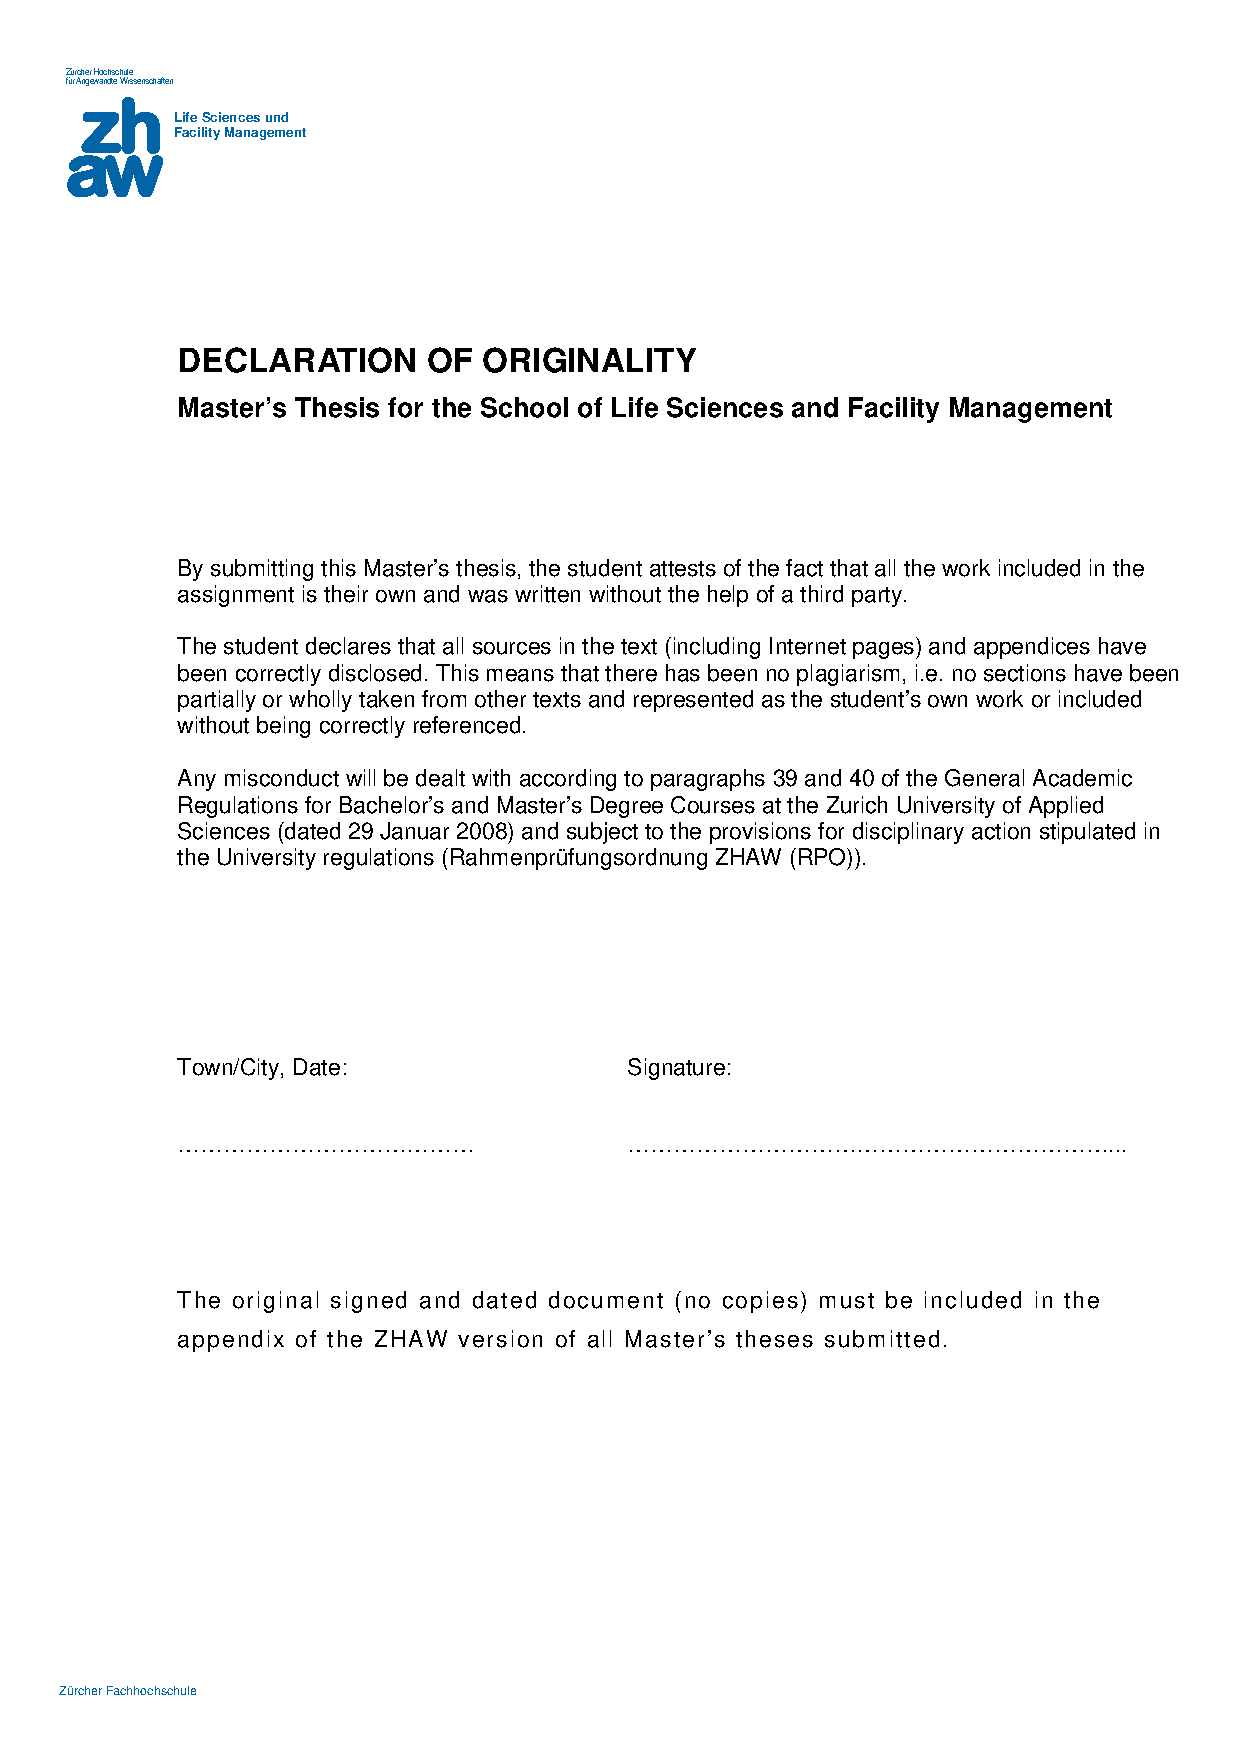
\includepdf[pages=-]{Appendices/plagiatserklaerung-master-eng.pdf}
 


%----------------------------------------------------------------------------------------
% BIBLIOGRAPHY
%----------------------------------------------------------------------------------------
\printbibliography[heading=bibintoc]

%----------------------------------------------------------------------------------------

\end{document}  
